%\documentclass[sigconf,nonacm]{acmart}
\documentclass[format=acmsmall, review=false]{acmart}

\usepackage{acm-ec-19}
\usepackage{booktabs} % For formal tables

%\usepackage[ruled]{algorithm2e} % For algorithms
%\renewcommand{\algorithmcfname}{ALGORITHM}
%\SetAlFnt{\small}
%\SetAlCapFnt{\small}
%\SetAlCapNameFnt{\small}
%\SetAlCapHSkip{0pt}
%\IncMargin{-\parindent}

\usepackage{booktabs} % For formal tables
\usepackage{amsmath,amssymb,amsfonts}
%Removed because of a conflict with LNCS style: amsthm
\usepackage[english]{babel}
\usepackage{xcolor}
\usepackage{tikz}
\usetikzlibrary{automata, graphs,positioning,chains,arrows,decorations.pathmorphing}
\usepackage{pgfplots}
\usepackage{pgfplotstable}
\usepackage{url}
\usepackage{subfigure}
\usepackage{comment}

%% Macros Juan

\newcommand{\paths}{\text{PATHS}}

%% Macros comments
\newcommand{\tover}[1]{\textcolor{red}{#1}}
\newcommand{\td}[1]{\textcolor{blue}{[TODO: #1]}}

%% Macros logics
\newcommand{\NN}{\mathbb{N}}
\newcommand{\ZZ}{\mathbb{Z}}
\newcommand{\MM}{\mathbb{M}}
\newcommand{\SE}{\mathbb{S}}
\newcommand{\BB}{\mathbb{B}}
\newcommand{\RR}{\mathbb{R}}
\newcommand{\cF}{\mathcal{F}}
\newcommand{\cI}{\mathcal{I}}
\newcommand{\QFBILIA}{\textsf{QFBILIA}}
\newcommand{\nnf}{\textsf{f}}

\newcommand{\ite}{\textsf{ite}}
\newcommand{\limp}{\Rightarrow}
\newcommand{\flc}{\rightarrow}

\newcommand{\bagone}[1]{\llbracket #1 \rrbracket}
\newcommand{\bsingle}{\textsf{bag}}
\newcommand{\bplus}{\oplus}
\newcommand{\bminus}{\ominus}

%% Macros tools
\newcommand{\spen}{\textsc{spen}}
\newcommand{\zzz}{\textsc{Z3}}

%% Environments
\newtheorem{mythm}{Theorem}[section]
\newtheorem{mydef}[mythm]{Definition}
\newtheorem{myprop}[mythm]{Proposition}
\newtheorem{mylem}[mythm]{Lemma}
\newtheorem{myex}[mythm]{Example}
\newtheorem{mycor}[mythm]{Corollary}

\newtheorem*{myrem}{Remark} %% based on amsthm
\newtheorem*{mynota}{Notation}
\newtheorem*{mylem*}{Lemma}
\newtheorem{myclaim}{Claim}
\newtheorem*{myclaim*}{Claim}
\newtheorem*{myprop*}{Proposition}
\newtheorem*{comp}{Efficiency Study}


\newenvironment{point}[1]
{\subsection*{#1}}%
{}

\newcommand{\flist}{\text{\sc FList}}
\newcommand{\set}{\text{\sc Set}}
\newcommand{\fset}{\text{\sc FSet}}
\newcommand{\B}{\text{\bf B}}
%\newcommand{\G}{\mathcal{G}}
\newcommand{\K}{\mathcal{K}}
\newcommand{\LOG}{\text{\sc Log}}
\newcommand{\length}{\text{\rm length}}
\newcommand{\BK}{\text{\sc BK}}
%\newcommand{\cP}{\mathcal{P}}
%\newcommand{\cV}{\mathcal{V}}
%\newcommand{\cC}{\mathcal{C}}
%\newcommand{\cS}{\mathcal{S}}
%\newcommand{\cA}{\mathcal{A}}
%\newcommand{\cR}{\mathcal{R}}
%\newcommand{\cQ}{\mathcal{Q}}
\newcommand{\cG}{\mathcal{G}}
\newcommand{\cT}{\mathcal{T}}
\newcommand{\pr}{\mathbf{Pr}}
\newcommand{\Dyck}{\mathcal{D}}
\newcommand{\expected}{\mathbf{E}}
\newcommand{\bv}{\mathbf{v}}
\newcommand{\bV}{\mathbf{V}}
\newcommand{\bs}{\mathbf{s}}
\newcommand{\bsigma}{\mathbf{\sigma}}
\newcommand{\bw}{\mathbf{w}}
\newcommand{\ba}{\mathbf{a}}
\newcommand{\bq}{\mathbf{q}}
\newcommand{\bx}{\mathbf{x}}
\newcommand{\by}{\mathbf{y}}

\newcommand{\bstring}{\{0,1\}^\ast}

\newcommand{\marcelo}[1]{{\color{red} {\bf Marcelo: #1}}}
\newcommand{\etienne}[1]{{\color{blue} {\bf Etienne: #1}}}
\newcommand{\juan}[1]{{\textcolor{violet} {\bf Juan: #1}}}
\newcommand{\domagoj}[1]{{\color{green} {\bf Domagoj: #1}}}
\newcommand{\francisco}[1]{{\color{magenta} {\bf Francisco: #1}}}
\newcommand{\martin}[1]{{\color{orange} {\bf Martin: #1}}}

\newcommand{\quot}[1]{#1/\!\equiv}

\newcommand{\then}{\,|\,}
\newcommand{\body}{q}
\newcommand{\bchain}{\text{bc}}
\newcommand{\epath}{\text{path}}

\newcommand{\owner}{\text{\rm owner}}
\newcommand{\pred}{\text{\rm pred}}
\newcommand{\mine}{\text{\rm mine}}
\newcommand{\suc}{\text{\rm succ}}


\newcommand{\bP}{\mathbf{P}}
\newcommand{\bB}{\mathbf{B}}
\newcommand{\bA}{\mathbf{A}}
\newcommand{\bR}{\mathbf{R}}
\newcommand{\bS}{\mathbf{S}}
\newcommand{\bH}{\mathbf{H}}
\newcommand{\bQ}{\mathbf{Q}}

\newcommand{\forkm}[1]{F^{#1}}
\newcommand{\mfork}{F_m}
\newcommand{\mgfork}{F_{m,g}}
\newcommand{\last}{\text{\rm last}}
\newcommand{\best}{\text{\rm best}}
\newcommand{\cho}{\text{\rm choose}}

\newcommand{\ie}{i.e.$\!$ }

\newcommand{\longest}{{\text{\rm longest}}}


\newcommand{\subbody}{{\text{\rm sub-state}}}

\newcommand{\cdf}{\text{\rm {\bf DF}}}
\newcommand{\df}{\text{\rm DF}}
\newcommand{\fg}{\text{\rm FG}}
\newcommand{\fr}{\text{\rm FR}}
\newcommand{\bdf}{\text{\rm {\bf DF}}}
\newcommand{\bfg}{\text{\rm {\bf FG}}}
\newcommand{\bfr}{\text{\rm {\bf FR}}}


%\newcommand{\af}{{\rm {F_\infty}}}
%\newcommand{\baf}{{\rm {\bf F_\infty}}}

\newcommand{\af}{\text{\rm AF}}
\newcommand{\baf}{\text{\rm {\bf AF}}}

\newcommand{\pf}[1]{\text{\rm F[{#1}]}}
\newcommand{\bpf}[1]{\text{\rm {\bf F}[{$#1$}]}}

\newcommand{\cat}{\text{\rm Catalan}}


\newcommand{\gup}{{\rm {G}}}
\newcommand{\bgup}{{\rm {\bf G}}}


\newcommand{\catalan}{{\rm {\it C}}}
%\newcommand{\dyck}{{\rm {\it D}}}


\newcommand{\meet}{\text{\rm meet}}

\DeclareMathOperator*{\argmax}{argmax}


%\newcommand{\rpa}{r_p^\alpha}
\newcommand{\rpa}{r_p}

\newcommand{\ameet}{\text{\rm all-meet}}
\newcommand{\base}{\text{\rm base}}

\newcommand{\ucl}{\text{\rm up-cl}}
\newcommand{\dcl}{\text{\rm down-cl}}

\newcommand{\pol}{\text{\it P}}





\allowdisplaybreaks

\begin{document}
\title{Cryptocurrency Mining through Stochastic Lenses}
\author{Submission ???[Add the number once assigned]}

\begin{abstract}
    In the consensus protocol used in most cryptocurrencies, participants called \emph{miners} are expected to perform actions for which they receive rewards. These actions consist on finding \emph{valid blocks} of transactions and appending them to a shared tree-like data structure. Ideally, the rules of the protocol should ensure that miners maximize their gains if they follow a default strategy, which consists on appending blocks only to the longest branch of the tree, called the \emph{blockchain}. This property is particularly important for the protocol as it ensures some desired properties related to security and stability. Unfortunately, existing models studying the optimal behavior of miners consider simplified reward functions, where the utility of a miner is the proportion of valid blocks she manages to include in the blockchain. This does not consider two important factors. First, that in most cryptocurrencies the reward for finding a valid block decreases over time, and second, the fact that a miner naturally prefers to be rewarded earlier than later (the economic concept of discount). Considering these two factors in a model for studying cryptocurrency mining has proven to be a hard task, leaving us without a clear understanding of the optimal behavior of miners.

%Our goal is to understand under which circumstances are miners incentivised to fork the blockchain by mining on top of blocks which are not at the tail of the current chain. In other word we study what are the conditions for which the default mining behaviour is better than any branching strategy. We model mining in cryptocurrencies as a stochastic game in which players always try to produce new blocks, and have to immediately disclose them to other. The probability of a player producing a new block depends on the hash power of the player, that is, the proportion of the computational power he controls compared to the power of the entire network. We work under the assumption that a miner's pay-off increase as long as his blocks are part of the blockchain. Players then look to maximise their utility in the long run, and their best strategy depends on their hash power and the discount applied to the reward of each new block being mined. We show that  if no discount is offered, then miners do not have any incentive to fork, no matter how high their hash power is. On the other hand, when working with discounts similar to those in Bitcoin, miners can have an incentive to fork; however the minimal proportion of hash power for which it happens is close to half. 

    Our goal is to provide a model of cryptocurrencies that can help in understanding under which circumstances are miners encouraged to follow the default strategy. In other words, we study what are the conditions for which the default mining behaviour is better than any other strategy. We model mining in cryptocurrencies as an infinite stochastic game in which players always try to produce valid blocks. The probability of a player finding a valid block depends on his fraction of the computational power of the entire network. To model the fact that block rewards decrease over time, we study the limit situation in which a miner does not receive a full reward for a block if it stops being in the blockchain. More precisely, the reward for a block is divided into an infinite number of payments, and the miner loses some of them whenever the block does not belong to the blockchain. Since older blocks in the blockchain are easier to maintain, we also ensure that the penalty for a block leaving the blockchain decreases with time. This limit situation represents miners who have a strong incentive to put--and maintain--their blocks in the blockchain.
Miners then look to maximise their utility in the long run, and their best strategy depends on their hash power and the discount applied to the reward of each new block being mined. We show that  if no discount is applied, then miners do not have incentives to create new branches, no matter how high their hash power is. On the other hand, when working with discounts similar to those in Bitcoin, miners can have an incentive to create such branches; however the minimal proportion of hash power for which it happens is close to half. 


% =======
%
%
% In the consensus protocol used in most cryptocurrencies, participants are expected to perform actions for which they receive a reward. These actions consist of including blocks of transactions in a common structure, and they are colloquially known as mining. Protocols must ensure that mining is compatible with the reward schema: In particular, participants are expected to behave appropriately if they want to maximise their gains, that is, they are expected to mine on the longest branch of blocks, called the blockchain. Yet studying incentives behind mining actions in cryptocurrencies has proven a difficult task, leaving us without a clear understanding of the optimal behavior of miners.
%
% %Our goal is to understand under which circumstances are miners incentivised to fork the blockchain by mining on top of blocks which are not at the tail of the current chain. In other word we study what are the conditions for which the default mining behaviour is better than any branching strategy. We model mining in cryptocurrencies as a stochastic game in which players always try to produce new blocks, and have to immediately disclose them to other. The probability of a player producing a new block depends on the hash power of the player, that is, the proportion of the computational power he controls compared to the power of the entire network. We work under the assumption that a miner's pay-off increase as long as his blocks are part of the blockchain. Players then look to maximise their utility in the long run, and their best strategy depends on their hash power and the discount applied to the reward of each new block being mined. We show that  if no discount is offered, then miners do not have any incentive to fork, no matter how high their hash power is. On the other hand, when working with discounts similar to those in Bitcoin, miners can have an incentive to fork; however the minimal proportion of hash power for which it happens is close to half. 
%
% Our goal is to provide a model of mining in cryptocurrencies that can help in understanding the circumstances under which miners are incentivised to behave appropriately. In other words, we study what are the conditions for which the default mining behaviour is better than any other strategy. We model mining in cryptocurrencies as an infinite stochastic game in which players always try to produce new blocks, and must immediately disclose them to others. The probability of a player producing a new block depends on the hash power of the player, that is, the proportion of the computational power she controls compared to the power of the entire network. Moreover, we abstract from the different rules for rewarding miners in different cryptocurrencies, and we focus on the limit situation in which a miner does not receive a full reward for a block if it stops being in the blockchain. More precisely, the reward for a block is divided into an infinite number of payments, and the miner loses some of them whenever the block does not belong to the blockchain. Since older blocks in the blockchain are easier to maintain, we also ensure that the penalty for a block leaving the blockchain decreases with time. This limit situation represents miners who have a strong incentive to put--and maintain--their blocks in the blockchain.
% Miners then look to maximise their utility in the long run, and their best strategy depends on their hash power and the discount applied to the reward of each new block being mined. We show that  if no discount is applied, then miners do not have any incentive to create new branches, no matter how high their hash power is. On the other hand, when working with discounts similar to those in Bitcoin, miners can have an incentive to create such branches; however, the minimal proportion of hash power for which it happens is close to half. 
% >>>>>>> 0c0682dde50426298d75c57b49c5ee95af8926f4
\end{abstract}



\maketitle

%!TEX root = ../main/main.tex

\section{Introduction}

The Bitcoin Protocol \cite{Bitcoin,DBLP:books/daglib/0040621,NC17}, or Nakamoto Protocol, introduces a novel decentralized network-consensus mechanism that is trustless and open for anyone connected to the Internet. This open and dynamic topology is supported by means of an 
%To support such an open and dynamic topology, the protocol requires an 
underlying currency (a so-called \emph{cryptocurrency} \cite{NC17}), to encourage/discourage participants to/from taking certain actions. The largest network running this protocol at the time of writing is the Bitcoin network, and its underlying cryptocurrency is Bitcoin (BTC). The success of Bitcoin lead the way for several other cryptocurrencies; some of them 
%Following the success of Bitcoin, several other cryptocurrencies have been created. Some of them 
are replicas of Bitcoin with slight modifications (e.g. Litecoin%\footnote{\url{https://litecoin.org}}
~\cite{Litecoin} 
or Bitcoin Cash%\footnote{\url{https://www.bitcoincash.org}}),
~\cite{Bcash}), 
while others introduce more involved modifications 
%introduce more involved  interesting new modifications on top of the protocol to provide further functionalities 
(e.g. Ethereum%\footnote{\url{https://ethereum.org}}
~\cite{Ethereum,E17} 
or Monero%\footnote{\url{https://getmonero.org}}).
~\cite{Monero}).

The data structure used in these protocols is an append-only record of transactions, which are assembled into \emph{blocks}, and appended to the record once they 
are marked as valid. The incentive to generate valid new blocks is an amount of currency, which is known as the \emph{block reward}. 
In order to give value to the currencies, the 
%But then this means that generating 
%new blocks must be hard. Under the 
proof-of-work framework mandates that participants generating new blocks are required to solve some computationally hard problem per each new block.  This is known as \emph{mining}, and the number of problems per second that a miner can solve is referred to as her \emph{hash power}. Agents who participate in the generation of blocks are called \emph{miners}. In Bitcoin, for example, the hard problem corresponds to finding blocks with a hash value that, when interpreted as a number, is less than a certain threshold. Since hash functions are pseudo-random, the only way to generate a valid block is to try with several different blocks, until one of them has a hash value below the established threshold. 

Miners are not told where to append the new blocks they produce. The only requirement is that new blocks must include a pointer to a previous block in the data structure, 
which then naturally forms a tree of blocks. The consensus data structure is generally defined as the longest branch of such a tree, also known as the \emph{blockchain}. In terms of cryptocurrencies, this means that the only valid currency should be the one that originates from a 
%transaction or a block reward in a 
block in the blockchain. 
%
%The data structure used in these protocols is an append-only record of transactions, and one of its most important components is the way new transactions 
%are  verified and appended to the record. Typically, transactions are assembled into \emph{blocks}, which become candidates to be appended to the record once they are 
%marked as valid. 
%%Apart from the set of transactions, the block will contain a pointer to some previous block, so that the record naturally forms a tree of blocks. 
%%The consensus data structure is generally defined as the longest branch of such a tree, also known as the \emph{blockchain}.
%To provide an incentive to generate and verify these new blocks, protocols reward agents creating new blocks with an amount of currency, which is known as the \emph{block reward}, and it is also the way in which new currency is created. For example, in Bitcoin this amount was originally 50BTC and halves approximately every four years, which is informally known as Bitcoin's \emph{deflation} (the current reward is 12.5BTC). 
%But since blocks give a reward, nodes will naturally want to generate blocks 
%Thus, agents would naturally want to generate blocks. If we expect the currency to have any value, generating new blocks must then be hard. Under the proof-of-work framework, participants generating new blocks are required to solve some computationally hard problem per each new block.  This is known as \emph{mining}, and the number of problems per second that a miner can solve is referred to as her \emph{hash power}. Agents who participate in the generation of blocks are called \emph{miners}. Coming back to the Bitcoin example, the hard problem corresponds to finding blocks with a hash value that, when interpreted as a number, is less than a certain threshold. Since hash functions are pseudo-random, the only way to generate a valid block is to try with several different blocks, until one of them has a hash value below the established threshold. 
%
%
%Miners are not told where to append the new blocks they produce. The only requirement is that new blocks must include a pointer to a previous block in the data structure, 
%which then naturally forms a tree of blocks. The consensus data structure is generally defined as the longest branch of such a tree, also known as the \emph{blockchain}. 
%In terms of cryptocurrencies, this means that the only valid currency should be the one that originates from a transaction or a block reward in a block in the blockchain.\footnote{In order to encourage including all the transactions that are correct according to the cryptocurrency rules, the miners also receive a small {\em transaction fee} for each transaction they include in a block. As in currently used cryptocurrencies fees rarely exceed 10\% of the mining reward \cite{TotalMiningRevenue,TotalMiningFees}, we focus on block rewards when gauging the miner's economic motivation for participating in the protocol.}
%, the longest branch in the tree. 
%Protocols normally add additional rules to specify when a currency is ready to be spent. In Bitcoin, for example, a block reward is considered ready to spend only when there are 
%at least 100 blocks appended after it in the blockchain.
%
Miners looking to maximise their rewards may then attempt to create new branches out of the blockchain, to produce a longer branch that contains more of their blocks (and earn more block rewards) or to produce a branch that contains less blocks of a user they are trying to harm. This opens up several interesting questions: under what circumstances are miners 
encouraged to produce a new branch in the blockchain? What is the optimal strategy of miners assuming they have a rational behaviour? %Also, since certainly a mining war is undesirable for a cryptocurrency, 
Finally, how can we design new protocols where miners do not have incentives to deviate from the main branch? 


%As far as I know, nobody has a good model of how miners cash out their coins, and we cannot say that it is the best to cash out as soon as coins are available according to the protocol (for example, if they are in a block in the blockchain with 100 blocks further ahead), in particular given the volatility that you mention. Given this, we want to study the limit situation where there is a penalty for a miner if a block stops being in the blockchain, and he does not receive all the payment for this block. We also want to include the condition that the penalty decreases with time (the longer the block is in the blockchain, the smaller the penalty). The interesting question then is whether in a limit situation like this it can still be convenient for the miners to fork, and the interesting thing is that the answer is yes when the payment per block decreases with time (the use of alpha). This confirms the results obtained before but with a much stronger assumption.

Our goal is to provide a model of mining that can incorporate different types of block rewards (including the decreasing rewards used in e.g. Bitcoin, where rewards for block decrease after a certain amount of time), as well as the economic concept of \emph{discount}, i.e. the fact that miners prefer to be rewarded sooner than later, and that can help in answering the previous questions. 
Since mining protocols vary with each cryptocurrency, 
%With each cryptocurrency adding new rules and parameters to mining protocols, 
distilling a clean model that can answer these questions while simultaneously covering 
all practical nuances of currencies is far from trivial~\cite{mininggames:2016}. 
Instead, we abstract from these rules and focus on the limit situation in which a miner does not receive the full reward for a block if it stops being in the blockchain. 
%, thus imposing a strong incentive for miners to put their blocks in the blockchain. 
More precisely, the reward for a block $b$ is divided into an infinite number of payments, and the miner loses some of them whenever $b$ does not belong to the blockchain. 
%The penalty decreases over time, so that the newer a block is, the more important it is to maintain it in the blockchain. 
%. The economic discount also ensures that 
%Since older blocks in the blockchain could have already been cashed-out, we ensure that 
%the penalty for a block leaving the blockchain decreases over time. 
This limit situation represents miners with a strong incentive to put--and maintain--their blocks in the blockchain, and is relevant when studying cryptocurrencies
as a closed system, where miners do 
not wish to spend money right away but rather be able to cash-out their wealth at any point in time. 
%
% , which ensures that miners are rewarded according to the effort put into maintaining their blocks in the blockchain.
%%Our goal is to produce a model of mining in a cryptocurrency that can help in answering these questions. 
%%With several cryptocurrencies bringing new rules and parameters to these questions, distilling a clean model that can answer these questions while simultaneously covering 
%%all practical nuances of currencies is far from being trivial~\cite{mininggames:2016}. 
%%Instead, 
%%we abstract from these rules and focus on the limit situation in which a miner does not receive a full reward for a block if it stops being in the blockchain, thus imposing a strong incentive for miners to put their blocks in the blockchain. In other words, the full reward for a block $b$ is divided into several payments, and the miner loses some of them when $b$ does not belong in the blockchain. 
%%Since we do not want to impose a limit on the time in which a cryptocurrency is going to be used, we assume that the reward for a block $b$ is divided into an infinite number of payments, and we also suppose that the penalty for a block leaving the blockchain decreases with time. This latter condition is used to ensure that miners are rewarded according to the effort put into maintaining their blocks in the blockchain.
%
%In our work, this incentive takes the form of a discounted utility.
%
In terms of how mining is performed, we consider these two simple rules: each player $i$ is associated
%Moreover, in our formalization of mining in a cryptocurrency,
%a scenario where the wealth of players is simply given by the number of blocks they have on the blockchain. More precisely, our game is based solely on the following rules. 
%we consider two other simple rules: each player $i$ 
%\begin{enumerate}
%\item 
%player $i$ 
a fixed value $h_i$ specifying her proportion of the hash power 
%of $i$
%this player 
against the total hash power, and  
%\item 
%In each step, 
%each player tries 
she tries in each step to append a new block somewhere in the tree of blocks, being 
%The 
%probability that player $i$ succeeds is $h_i$.
$h_i$ her probability of succeeding. 
%\item The utility of players depend on how many blocks they have in the blockchain: in every step they want to have as many blocks as possible in the blockchain.
%\end{enumerate}
%\noindent

The last two rules mentioned above 
%The first two rules 
are the standard way of 
%simulating 
formalizing mining in a cryptocurrency 
%game 
%when assuming that each player controls a fixed amount of hash power. 
On the other hand, the way a miner is rewarded for a block in our model
% third rule complies with the idea that the wealth in our model is given by the number of blocks in the blockchain. This framework is relevant when studying cryptocurrencies as a closed system, where miners do not wish to spend the money right away but rather simply accumulate wealth in 
%this cryptocurrency, for example because they speculate a price increase in the long term, or because they want to be able to cash-out their wealth at any point in time. As our framework allow us to consider any potential branching strategy, even one which endanger the trust in the cryptocurrency, it is fair to assume that the real world value of the currency can be really volatile, hence the incentive for a miner to be able cash-out at any point.
%We remark that this framework 
takes us on a different path from most of current literature, wherein agents typically mine 
%looks to mine 
with the objective of cashing-out as soon as possible or after an amount of time chosen a priori   \cite{mininggames:2016,biais2018blockchain}. Far from being orthogonal, our framework is complementary with these studies, as it allows to validate some of the assumptions and results obtained in these articles with miners who have stronger motives to mine and keep their blocks in the blockchain.
%the assumptions upon which their models are based. 


\noindent{\bf Contributions.}  Our first contribution 
%is to provide a
is a model for blockchain mining, given as an infinite stochastic game in which maximising the utility corresponds to both 
putting blocks in the blockchain and maintaining them there for as long as possible. A
%One of the 
benefit of our model is that using few basic design parameters we can 
%in fact 
accommodate different cryptocurrencies, and not focus solely on Bitcoin,
% These parameters also 
while also allowing us to account for fundamental factors such as deflation, or discount in the block reward. 
Moreover as our model gives a fair payoff to each miner when a mining race occurs, it allow us to study the validity of the commonly accepted assumption that long fork are not a viable strategy.
%  Besides,
%  we can reason about all possible branching strategies in our proposal, 
%  without the need to focus on a specific subclass. 
The second contribution of our work is a set of results about optimal strategies in two different scenarios. First, 
we study mining under the assumption that block rewards are constant (as it will eventually be in cryptocurrencies with tail-emission such as Monero or Ethereum), and secondly, assuming that per-block reward decreases over time (a continuous approximation to Bitcoin rewards). 

In the first scenario of constant rewards, we show that the default strategy of always mining on the latest block of the blockchain is indeed a Nash equilibrium and, in fact, 
provides the highest possible utility for all players. Therefore with constant reward, we prove that long forks should not happen, as it is not an optimal strategy. 
%This means that, if miners want to accumulate wealth in terms of the same currency  or if it is important for them to be able to cash-out at any time, they should not fork. Moreover, this result shows that, with constant reward, the commonly accepted assumption that long forks should not happen is true. 
On the other hand, if block reward decreases over time, we prove that strategies that involve forking the blockchain
can be a better option than the default strategy, and thus we study what is the best strategy for miners when assuming everyone else 
is playing the default strategy. We provide different strategies that involve branching at certain points of the blockchain, and show how to compute their 
utility. When we analyse which one of these strategies is the best, we see that the choice depends on the hash power, the rate at which 
block rewards decrease over time, and the usual financial discount rate. We confirm the commonly held belief that
players should start deviating from the default strategy 
when they approach 50\% of the network's hash power (also known as 51\% attack), but we go further: there are more complex strategies that 
prove better than default even with less than 50\% of the hash power. 
Further investigation is needed but these results complement and improve our current understanding of mining strategies and tend to show that even with decreasing reward long forks should not happen if no miner is holding close to 50\% of the hash power, therefore validate the assumption used in most previous works (see e.g. \cite{mininggames:2016,biais2018blockchain}).

%We study what is the best strategy for miners when assuming everyone else is playing the default strategy. As we see, the 
%choice of a better strategy here depends on the hash power, the rate at which 
%block rewards decrease over time, and the usual financial discount rate. This confirms once again the commonly held belief that
%players should start deviating from the default strategy 
%when they approach 50\% of the network's hash power (also known as 51\% attack). Going further, we devise more complex strategies that 
%prove better than default with a bit less than 50\% of hash power. 
%These results tend to show that, with decreasing reward, the assumption that long forks should not happen holds upon reasonable hash power repartition.


\noindent{\bf Related work.} Our framework takes us on a different path that most of current literature offering a game-theoretic characterisation for blockchain mining \cite{mininggames:2016,biais2018blockchain,koutsoupias2018blockchain}, which typically model the reward of players as the proportion of their blocks with respect to the total number of blocks (we pay for each block). Each choice has its own benefits; our choice allows us to analyse different forms of rewards and also introduce a discount factor on the utility, which we view as one of the main advantages of our model. It is also common to introduce assumptions that limit the set of strategies. For instance, Kiayias et.al. \cite{mininggames:2016} assume that only one block per depth generates reward, which is natural in their framework but limits the set of valid strategies they consider. Moreover, Biais et.al.\cite{biais2018blockchain}  assume that the reward of a block depends on the proportion of hash-power dedicated to blockchains containing it at a time chosen a priori. These assumptions do not take into account every potential forking strategies, or the fact that a miner may want to adapt his cash-out strategy based on the situation. 
% One thing we are not considering in this paper, and are considered in these previous works, is strategies that feature a strategic release of blocks, in which miners opt not to release new blocks in hope that these will give them a future advantage.
Lastly, our framework cannot deal with strategies that feature a tactical release of blocks often referred as selfish mining, in which miners opt not to release new blocks in hope that these will give them a future advantage \cite{optimalselfishmining2017,selfishmining2014,stop_selfish_mining2014,stubborn_mining:2016,stubborn_mining:2015}. 
Our model can be extended to account for most of those strategies, for example by defining states as a tuple of trees, one for each player. 
However work studying precise problems and taking into account the intrinsic cost of mining like electricity \cite{tsabary2018gap,biais2018blockchain} cannot easily be added to our framework, because it requires a continuous time-based model for mining.
%Something we are not considering in this article, and is considered in these previous works, is the set of strategies that feature a tactical release of blocks, in which miners opt not to release new blocks in hope that these will give them a future advantage. Our model can be extended to account for these strategies, for example by defining states as a tuple of trees, one for each player. We are currently looking into this extension and it is part of our future work. %We have opted not to include these options to preserve the readability of the paper. 
%In our work, we assume that the reward given to a block owner is distributed over time, as long as the block stays on the main chain. This, we believe, is adequate to study any possible branching strategy, due to the expected volatile cryptocurrency's value.
%Our results imply that long forks should not happen under reasonable hash-power distritutions, in which case we acknowledge that the assumptions made in the mentioned works are justified when the cryptocurrency value is considered stable.

Among other works that approach cryptocurrency mining from a game-theoretical point of view, we mention \cite{economics_of_mining2013,instabilitywithoutreward:2016}, noting that these differ from our work either in the choice of 
a reward function, the space of mining strategies considered, or both. 
As far as we are aware, our work is the first to provide a model that can account for multiple choices in the reward function (say, constant reward or decreasing reward), and without any assumption on the set of strategies.  Recently, the perks of adding new functionalities to bitcoin's mining protocol have been studied: In \cite{koutsoupias2018blockchain}, it is shown that a pay-forward option would ensure optimality of the default behaviour, even when miner rewards are mainly given as transaction fees.
There is also interesting work regarding mining strategies in multi-cryptocurrency markets \cite{dhamal2018stochastic,spiegelman2018game}, and a number of articles on network properties of the Bitcoin protocol, as well as technical considerations regarding its security and privacy (see e.g. the survey by Conti et al. \cite{conti2018survey}). Interestingly, 
%Remarkably, it is concluded that 
some network settings can inflict undesired mining behaviour ~\cite{bitcoin_attacks_2013,ddos_attacks2014,empirical_dos_attacks2014}.   
%Work studying precise problems and taking into the intrinsic cost of mining as electricity \cite{tsabary2018gap}, are not comparable 
% The main difference with our work is that we focus on a single cryptocurrency in a closed world setting (e.g. we do not reason about  the exchange rate of the studied cryptocurrency with the US dollar or another cryptocurrency). Finally, there are a number of papers on network properties of the Bitcoin protocol, as well as technical considerations regarding its security and privacy (see e.g. the survey by Conti et al. \cite{conti2018survey}). One interesting result here is that the network's specificity of the protocol could give participants an incentive to deviate from default behaviour~\cite{bitcoin_attacks_2013,ddos_attacks2014,empirical_dos_attacks2014}.   

%More specifically,  Kroll et al. \cite{economics_of_mining2013} focus on a subset of strategies they call \emph{monotonic}, and prove a 
%Nash equilibria for these strategies when assuming a constant payoff model. Eyal and Sirer~\cite{selfishmining2014}  and later Sapirshtein et al. in \cite{optimalselfishmining2017} studied a different strategy known as \emph{selfish mining}, in which miners may withhold some of their newly created blocks. Their main result is that, assuming that all other miners are following the default strategy and that block rewards remain constant, a miner with strictly less than 50\% of the network's hash power can increase his income by not always revealing block immediately (thus proving that the default strategy is not a Nash equilibrium). Carlsten et al. \cite{instabilitywithoutreward:2016} studied the \emph{tail} behavior of Bitcoin in which the block reward becomes negligible compared to the mining fees, proving that in such situation miners have further incentives to deviate from the default strategy. 
%%Those works differs from our's in that they consider a model with constant block's reward \cite{selfishmining2014,optimalselfishmining2017} or really volatile block's reward \cite{instabilitywithoutreward:2016}. 
%A formalisation considering a utility where miners must define a fixed cash-in window as they start the game has been studied in \cite{biais2018blockchain}, and the authors proved the existence of a non-default nash equilibrium in this set-up.
%Perhaps the study which is closest in spirit to ours is the one by Kiayias et al. in \cite{mininggames:2016}. %later on extended in \cite{biais2018blockchain}. 
%Here the authors also focus on the hash power thresholds for which the default strategy is not an optimal strategy any more. Albeit the authors consider a range of strategies, their model is still somewhat more restrictive than ours. %not able to consider the same as our. %\francisco{I do not understand this last phrase}

\noindent
{\bf Proviso.} Due to the lack of space, all proofs are provided in the appendix. 

%\smallskip
%\noindent
%{\bf Organization of the paper.} We present our game-theoretic formalization of cryptocurrency mining in Section \ref{sec-formalization}. Our results for constant and decreasing rewards are presented in Sections \ref{sec-const_rew} and~\ref{sec-dec}, respectively. Finally, some concluding remarks are given in Section~\ref{sec-con-r}. We provide the main details of the proofs of the results in the paper; however, due to the lack of space, complete proofs of all results are provided in an appendix.
%full version of this paper, which can be found at \url{https://anonymous.4open.science/repository/08eff11e-78b1-4836-837a-cff08348a8c8}. Besides, independent Python and C++ scripts used in the paper for the utility evaluation and plots generation can also be found in this repository.





%!TEX root = ../main/main.tex

\section{A Game-theoretic Formalisation of Crypto-Mining}
\label{sec-formalization}

%In what follows we define the components of the infinite stochastic game considered in this paper. 
The mining game is played by a set $\bP = \{0, 1, , \ldots, m-1\}$ of players, with $m \geq 2$.
In this game, each player gains some reward depending on the number of blocks she owns. Every block must point to a previous block, except for the first block which is called the {\em genesis block}. Thus, the game defines a tree of blocks. Each block is put by one player, called the {\em owner} of this block. Each such a tree is called a {\em state of the game}, or just {\em state}, and it represents the knowledge that each player has about the blocks that have been mined thus far.

The key question for each player is, then, where do I put my next block? The general rule in cryptocurrencies is that miners are only allowed to spend their reward if their blocks belongs to the \emph{blockchain}, which is simply the longest chain of blocks in the current state. Thus, players face essentially two possibilities: put their blocks right after the end of the blockchain, or try to \emph{fork}, betting that a smaller chain will eventually become the blockchain. As the likelihood of mining the next block is directly related to the comparative hash power of a player, we model mining as an infinite stochastic game, in which the probability of executing the action of a player $p$ is given by her comparative hash power.

In what follows we define the components of the game considered in this paper. Our formalisation is similar to others in the literature \cite{mininggames:2016,koutsoupias2018blockchain}, except for the way in which miners are rewarded and the way in which these rewards are accumulated in the utility function. These elements are fundamental in our formalisation. A detailed analysis of our reward can be found in Appendix \ref{sec-pay-uti}.
%Hence, we analyse them in more detail in Section \ref{sec-pay-uti}, emphasizing the properties of these two elements that are fundamental for our formalization.

% Let us now turn to the formal definition of the game.
%\vspace*{-15pt}
%\subsection{The definition of the game}
%\smallskip
%\noindent
\subparagraph*{Blocks, states and the notion of blockchain.}%\label{sub:states}
In a game played by $m$ players, a block is defined as a string $b$ over the alphabet $\{0,1,\ldots$, $m-1\}$. We denote by $\bB$ the set of all blocks, that is, $\bB = \{0,1,\ldots , m-1\}^*$. Each block apart from $\varepsilon$ has a unique owner, defined by the function $\owner: (\bB \smallsetminus \{\varepsilon\}) \rightarrow \{0,1, \ldots ,m-1\}$ such that $\owner(b)$ is equal to the last symbol of $b$. As in~\cite{mininggames:2016}, a state of the game is defined as a tree of blocks. More precisely, a state of the game, or just state, is a finite and nonempty set of blocks $q \subseteq \bB$ that is prefix closed. That is, $q$ is a set of strings over the alphabet $\{0,1,\ldots, m-1\}$ such that if $b\in q$, then every prefix of $b$ (including the empty word $\varepsilon$) also belongs to $q$. Note that a prefix closed subset of $\bB$ uniquely defines a tree with $\varepsilon$ as the root.
%
The intuition here is that each element of $q$ corresponds to a block that was put into the state $q$ by some player. The genesis block corresponds to $\varepsilon$. When a player $p$ decides to mine on top of a block $b$, she puts another block into the state defined by the string $b\cdot p$, where we use notation $b_1 \cdot b_2$ for the concatenation of two strings $b_1$ and $b_2$.
%
Notice that with this terminology, given $b_1, b_2 \in q$, we have that $b_2$ is a descendant of $b_1$ in $q$ if $b_1$ is a prefix of $b_2$, which is denoted by $b_1 \preceq b_2$. Moreover, a path in $q$ is a nonempty set $\pi$ of blocks from $q$ for which there exist blocks $b_1, b_2$ such that $\pi = \{ b \mid b_1 \preceq b$ and $b \preceq b_2\}$; in particular, $b_2$ is a descendant of $b_1$ and $\pi$ is said to be a path from $b_1$ to $b_2$.
Finally, let $\bQ$ be the set of all possible states in a game played by $m$ players, and for a state $q \in \bQ$, let $|q|$ be its size, measured as the cardinality of the set $q$ of strings (or blocks).

The {\em blockchain} of a state $q$, denoted by $\bchain(q)$, is the path $\pi$ in $q$ of largest length, in the case this path is unique.
%, in which case we denote it by $\bchain(q)$ \francisco{``in which case'' and ``in this case'' is redundant}. 
If two or more paths in $q$ are tied for the longest, then we say that the blockchain in $q$ does not exist, and we assume that $\bchain(q)$ is not defined (so that $\bchain(\cdot)$ is a partial function). %Notice that if $\bchain(q) = \pi$, then $\pi$ has to be a path in $q$ from the genesis block $\varepsilon$ to a leaf of~$q$.
%If the blockchain of $q$ is defined, say $b = \bchain(q)$, then a block $b' \in q$ is said to belong to the blockchain of $q$ if $b' \in \epath(b)$, that is, if $b'$ is a block in the path from the root $\varepsilon$ to $b$ in the state $q$.
%
\begin{example}\label{ex-mining}
Consider the following state $q$ of the game with players $\bP =\{0,1\}$:
\vspace*{-9pt}
\begin{center}
\begin{tikzpicture}[->,>=stealth',auto,thick, scale = 0.55,state/.style={circle,inner sep=2pt}]
	\node [state] at (-0.2,0) (r) {$\varepsilon$};
	\node [state] at (1.5,0.75) (n0) {$0$};
	\node [state] at (1.5,-0.75) (n1) {$1$};
	\node [state] at (3.3,-0.75) (n11) {$11$};
	\node [state] at (5.4,0) (n110) {$110$};
	\node [state] at (5.4,-1.5) (n111) {$111$};
	\node [state] at (7.7,-1.5) (n1111) {$1111$};
	\node [state] at (10.2,-1.5) (n11110) {$11110$};

	\path[->]
	(r) edge (n1)
	(r) edge (n0)
	(n1) edge (n11)
	(n11) edge (n110)
	(n11) edge (n111)
	(n111) edge (n1111)
	(n1111) edge (n11110);
\end{tikzpicture}
\end{center}
\vspace*{-9pt}
In this case, we have that $q = \{\varepsilon, 0, 1, 11, 110, 111, 1111, 11110\}$, so $q$ is a finite and prefix-closed subset of $\bB = \{0,1\}^*$. The owner of each block $b \in q \smallsetminus \{ \varepsilon\}$ is given by the the last symbol of $b$; for instance, we have that $\owner(11) = 1$ and $\owner(11110) = 0$. Moreover, the longest path in $q$ is $\pi = \{\varepsilon, 1, 11, 111, 1111, 11110\}$, so that the blockchain of $q$ is $\pi$ (in symbols, $\bchain(q) = \pi$).
%Thus, we have that the blocks that belong to the blockchain of $q$ are $\varepsilon$, $1$, $11$, $111$, $1111$, $11110$, since these are precisely the blocks in $q$ in the path from $\varepsilon$ to $11110$ (in symbols, $\epath(\bchain(q)) = \{\varepsilon, 1, 11, 111, 1111, 11110\}$). Notice that the information about these blocks is important as the reward of each player depends on the blocks that belong to her in the blockchain. For instance, if the reward for each block is a constant $c$, then we have that the reward of player 1 is $4 c$ in $q$, as four blocks in the blockchain of $q$ belong to this player.
Finally, 
%notice that 
$|q| = 8$, as $q$ is a set consisting of eight blocks (including the genesis block $\varepsilon$). 

	Assume now that $q'$ is the following state of the game:
	\begin{center}
\begin{tikzpicture}[->,>=stealth',auto,thick, scale = 0.55,state/.style={circle,inner sep=2pt}]
	\node [state] at (-0.2,0) (r) {$\varepsilon$};
	\node [state] at (1.5,0.75) (n0) {$0$};
	\node [state] at (1.5,-0.75) (n1) {$1$};
	\node [state] at (3.3,-0.75) (n11) {$11$};
	\node [state] at (5.4,0) (n110) {$110$};
	\node [state] at (7.6,0) (n110x) {$\cdots$};
	\node [state] at (10.4,0) (n110x0) {$11\underbrace{0\cdots0}_{n}$};
	\node [state] at (5.4,-1.5) (n111) {$111$};
	\node [state] at (7.6,-1.5) (n111x) {$\cdots$};
	\node [state] at (10.4,-1.5) (n111x1) {$11\underbrace{1\cdots1}_{n}$};

	\path[->]
	(r) edge (n1)
	(r) edge (n0)
	(n1) edge (n11)
	(n11) edge (n110)
	(n110) edge (n110x)
	(n110x) edge (n110x0)
	(n11) edge (n111)
	(n111) edge (n111x)
	(n111x) edge (n111x1);
\end{tikzpicture}
\end{center}
\vspace{-10pt}
%In this case, 
We have that $\bchain(q')$ is not defined since the paths $\pi_1 = \{\varepsilon, 1, 11, 110, \cdots, 110^n\}$ and $\pi_2 = \{\varepsilon, 1, 11, 111, \cdots, 111^n\}$ are tied for the longest path in $q'$. \qed
\end{example}


%Real-life cryptocurrencies also contain transactions that indicate movement of money in the system, and thus there are
%several different blocks that a player $p$ can use to extend the current state when mining upon a block $b$ (e.g., depending on the ordering of transactions).%
%%, or the nonce being used to announce the block). 
%Since we are interested %primarily 
%in miners behaviour, we just focus on the owner of the block following $b$, and do not consider the possibility of two different blocks belonging to $p$ being added on top of $b$. 
%%Alternatively, if we consider the Bitcoin protocol, we could say that all the different blocks that $p$ can put on top of $b$ are considered as~equivalent.
%%\juan{moving this to the reward section}
%%\etienne{We may have to specify that it is under the assumption that there are no fees or that they are negligible.} \marcelo{Etienne is right about this, depending on the transactions included in the block the reward could be different. I don't think we should talk about reward here.}

%\noindent
\subparagraph*{Actions of a miner.} %\label{sub:actions}
On each step, each miner
% looking to maximize their rewards 
chooses a block in the current state, and attempts to mine on top of this block. Thus, in each turn, each of the players race to place the next block in the state, and only one of them succeeds. The probability of succeeding is directly related to the comparative amount of hash power available to this player, the more hash power the more likely it is that she will mine the next block. %before the rest of the players. 
Once a player places a block, this block is added to the current state, obtaining a different state from which the game continues.

Let $p \in \bP$. Given a block $b \in \bB$ and a state $q \in \bQ$, we denote by $\mine(p,b,q)$ an action in the mining game in which player $p$ mines on top of block $b$. Such an action $\mine(p,b,q)$ is considered to be valid if $b \in q$ and $b\cdot p \not\in q$. The set of valid actions for player $p$ is collected in the~set:
\begin{eqnarray*}
\bA_p & = & \{ \mine(p,b,q) \mid b \in \bB, q \in \bQ \text{ and } \mine(p,b,q) \text{ is a valid action}\}.
\end{eqnarray*}
Moreover, given $a \in \bA_p$ with $a = \mine(p,b,q)$, the result of applying $a$ to $q$, denoted by $a(q)$, is defined as the state $q \cup \{b \cdot p\}$. Finally, we denote by $\bA$ the set of combined actions for the $m$ players, that is, $\bA = \bA_0 \times \bA_1 \times \cdots \times \bA_{m-1}$.

%\smallskip
%\noindent
\subparagraph*{Miner's Pay-off.}
%The next and last component of our game is the reward for miners: how much do they earn for each mined block. 
Most cryptocurrencies follow these rules for miner's payment:
%, and Bitcoin in particular. 
%
%\noindent
(1) Miners receive a possibly delayed one-time reward per each block they mine. %(in Bitcoin it is 12.5BTC at the time of writing).
%
%\noindent
(2) The only blocks that are valid are those in the blockchain; if a block is not in the blockchain then the reward given for mining this block cannot be spent. 
%%%%%MARCELO: remove the next sentence to avoid mentioning Bitcoin
%To prevent drastic changes on what are valid blocks, the Bitcoin protocol enforces that a block reward can only be spent when there are more than one hundred blocks on top of it. 

The second rule enforces that we cannot just give miners the full block reward when they put a block at the top of the current blockchain or after a delay, because invalid blocks may eventually give the same reward as valid ones. To illustrate this, consider the state $q'$ in Example \ref{ex-mining}, where we have two paths ($\pi_1$ and $\pi_2$) competing to be the blockchain, and consider $\pi_2$ to be the latest path to be mined upon to reach $q'$. If player $0$ had already been fully paid for any blocks $110^i$, where $i \leq n$, then if $\pi_2$ win the race and becomes the blockchain, such block $110^i$ would become invalid but still has given full reward to player $0$. To the best of our knowledge other attempts to formalize mining, especially bitcoin's mining partially emancipate from this rule, as only the first block to be confirmed will be paid, and artificially nullify the incentive to engage in long races.

%In Section \ref{sec-pay-uti}, we explain how our pay-off model can be used to pay for blocks and at the same time to ensure that players try to maintain their blocks in the blockchain. 
In the following sections we will show how different reward functions can be used to understand different mining scenarios that arise in different cryptocurrencies. 
For now we assume, for each player $p \in \bP$, the existence of a reward function $r_p : \bQ \to \mathbb{R}$ such that the reward of $p$ in a state $q$ is given by $r_p(q)$. Moreover, the combined reward function of the game is $\bR = (r_0, r_1, \ldots, r_{m-1})$. We also refer to the appendix (Section \ref{sec-pay-uti}) for an explanation on how 
our pay-off model can be used to pay for blocks and at the same time to ensure that players try to maintain their blocks in the blockchain.


%This can then allow a malicious miner (1 in this example) to do a local fork (e.g. the block 111), where for instance some transactions are being blocked, and does not provide an incentive for other miners to protect the other branch competing to be the blockchain. The way that the Bitcoin protocol goes around this is by paying for blocks which are buried deep into the blockchain.
% (they have been confirmed one hundred times). 
%This now gives a strong incentive to player 0 to mine on top of the block 110, since she cannot cash in her reward immediately after mining this block, but only once it has been extended many times.



%So how should the reward function look like? The first naive idea is to give miners the block reward as soon as they put a block at the top of the current blockchain. This provides some incentive to extend the blockchain, however, it does not completely protect the system from forks that other miners might want to initiate. To illustrate this, consider the state $q'$ in Example \ref{ex-mining}, where we have two blocks (110 and 111) competing to be in the blockchain, and consider 111 to be the last block added to reach $q'$. If player 0 already cashed in the reward for the block 110 (since this was awarded immediately), she has no further incentive to mine on top of this block, as the block 1110 would give her an equal reward. This can then allow a malicious miner (1 in this example) to do a local fork (e.g. the block 111), where for instance some transactions are being blocked, and does not provide an incentive for other miners to protect the other branch competing to be the blockchain. The way that the Bitcoin protocol goes around this is by paying for blocks which are buried deep into the blockchain.
% (they have been confirmed one hundred times). 
%This now gives a strong incentive to player 0 to mine on top of the block 110, since she cannot cash in her reward immediately after mining this block, but only once it has been extended many times.

%\smallskip
%\noindent
\subparagraph*{Transition probability function.} %\label{sub:transi}
As a last component of the game, we assume that $\pr : \bQ \times \bA \times \bQ \to [0,1]$ is a transition probability function satisfying that for every state $q \in \bQ$ and combined action $\ba = (a_0, a_1, \ldots, a_{m-1})$ in $\bA$, we have that $\sum_{p=0}^{m-1} \pr(q, \ba, a_p(q)) = 1$.

%As a last component of the game, we assume that $\pr : \bQ \times \bA \times \bQ \to [0,1]$ is a transition probability function satisfying that for every state $q \in \bQ$ and combined action $\ba = (a_0, a_1, \ldots, a_{m-1})$ in $\bA$:
%\begin{eqnarray*}\label{eq-prop}
%\sum_{p=0}^{m-1} \pr(q, \ba, a_p(q)) & = & 1.
%\end{eqnarray*}
Notice that if $p_1$ and $p_2$ are two different players, then for every action $a_1 \in \bA_{p_1}$, every action $a_2 \in \bA_{p_2}$ and every state $q \in \bQ$, it holds that $a_1(q) \neq a_2(q)$. Thus, we can think of $\pr(q, \ba, a_p(q))$ as the probability that player $p$ places the next block, which will generate the state $a_p(q)$. As we have mentioned, such a probability is directly related with the hash power of player $p$, the more hash power the likely it is that action $a_p$ is executed and $p$ mines the next block before the rest of the players. In what follows, we assume that the hash power of each player does not change during the mining game, which is captured by the following condition:
%\begin{itemize}
%\item Given $q, q' \in \bQ$ and $\ba, \ba' \in \bA$ with $\ba = (a_0, a_1$, $\ldots$, $a_{m-1})$ and $\ba' = (a'_0, a'_1, \ldots, a'_{m-1})$, for every player $p \in \bP$ it holds that $\pr(q, \ba, a_p(q)) = \pr(q', \ba', a'_p(q'))$.
%\end{itemize}
%Thus, we assume from now on that this condition is satisfied. In particular, 
for each player $p \in \bP$, we 
%assume that 
have that $\pr(q, \ba, a_p(q)) = h_p$ for every $q \in \bQ$ and $\ba \in \bA$ with $\ba = (a_0, a_1, \ldots, a_{m-1})$. We refer to such a fixed value $h_p$ 
%and we refer to $h_p$ 
as the hash power of player $p$.
%Moreover, we define $\bH = (h_0, h_1, \ldots, h_{m-1})$ as the hash power distribution, and we replace $\pr$ by $\bH$ in the definition of an an infinite stochastic game, so that $\Gamma = (\bP,\bA,\bQ,\bR,\bH)$.
Moreover, we assume that $h_p > 0$ for every player $p \in \bP$, as if this not the case then $p$ can be removed from the game.


%\smallskip
%\noindent
\subparagraph*{The mining game: definition, strategy and utility.}
Putting together all the components,  
%the components defined in the previous sections, 
%Summing up, from now on we consider 
a mining game is a tuple $(\bP,\bQ,\bA,\bR,\pr)$, where $\bP$ is the set of players, $\bQ$ is the set of states, $\bA$ is the set of combined actions, $\bR$ is the combined pay-off function 
and $\pr$ is the transition probability function. 
%The pay-off function of the game denoted $\bR = (r_0,r_1 \cdots, r_{m-1})$, with $r_p : \bQ \mapsto \mathbb{R^+}$ is the pay-off function of the player $p$, represent the reward that each player receive at any state of the game. Before presenting our model for the pay-off function we have to talked about the purpose of using stochastic game as a model.
%We have defined a game that can capture miners' interactions. A fundamental component of such a game is the strategy that each player decides to take, which combined determine the utility of each player. 
%In particular, miners take actions and decide about strategies trying to maximize their utility. In this sense, a 
%stationary 
%equilibrium of the game is a fundamental piece of information about miners' behavior, because such an equilibrium is a combination of players' strategies where no miner has an %incentive to perform a different action. 
%The notions of strategy, utility and stationary equilibrium are the last components of our game-theoretical characterisation of mining in Bitcoin, and they are defined next. 

A strategy for a player $p \in \bP$ is a function $s : \bQ \rightarrow \bA_p$.
We define $\bS_p$ as the set of all strategies for player $p$, and $\bS = \bS_0 \times \bS_{1} \times \cdots \times \bS_{m-1}$ as the set of combined strategies for the game (recall 
%that we are assuming 
that $\bP = \{0, \ldots, m-1\}$ is the set of players).
%As usual, we are interested in understanding which strategies are better than others, which we capture by the notions of utility and equilibrium. 
To define the notions of utility and equilibrium, we need some additional notation.
Let $\bs = (s_0, \ldots, s_{m-1})$ be a combined strategy.
% in $\bS$. 
Then given $q \in \bQ$, define $\bs(q)$ as the combined action $(s_0(q), \ldots, s_{m-1}(q))$. Moreover, given an initial state $q_0 \in \bQ$,
the probability of reaching state $q \in \bQ$, denoted by $\pr^{\bs}(q \mid q_0)$, is defined as 0 if $q_0 \not\subseteq q$ (that is, if $q$ is not reachable from $q_0$), and otherwise it is recursively defined as follows: if $q = q_0$, then $\pr^{\bs}(q \mid q_0) = 1$; otherwise, we have that $|q| - |q_0| = k$, with $k \geq 1$, and
$$
\pr^{\bs}(q \mid q_0) =
\sum_{\substack{q' \in \bQ \,:\\ q_0 \subseteq q' \text{ and } |q'| - |q_0| = k-1}}
 \pr^{\bs}(q' \mid q_0) \cdot \pr(q', \bs(q'), q).
 $$
In this definition, if for a player $p$ we have that $s_p(q') = a$ and $a(q') = q$, then $\pr(q', \bs(q'), q) = h_p$. Otherwise, we have that $\pr(q', \bs(q'), q) = 0$ 
(this is well defined since there can be at most one player $p$ whose action in the state $q'$ leads us to the state $q$). 
%. Notice that this is well defined, since there can be at most one player $p$ whose action in the state $q'$ leads us to the state $q$. 
For readability we write $\pr^{\bs}(q)$ instead of $\pr^{\bs}(q \mid \{\varepsilon\})$ to denote the probability of reaching state $q$ from the intial state $\{\varepsilon\}$ that contains 
only the genesis block  $\varepsilon$. 
%(consisting only of the genesis block $\varepsilon$).
%For the sake of presentation, the probability of reaching a state $q$ from the initial state $\{\varepsilon\}$ (consisting only of the genesis block $\varepsilon$) is denoted by $\pr^{\bs}(q)$, instead of $\pr^{\bs}(q \mid \{\varepsilon\})$. 
%Hence, consistently with the simplification described before, we can replace the transition probability function $\pr$ by the hash power distribution $\bH$ when computing $\pr^{\bs}(q \mid q_0)$.
%It should be noticed that 
%The framework just described corresponds to a Markov chain; in particular, the probability of reaching a state from an initial state is defined in the standard way for Markov chains~\cite{MU05}. However, we are not interested in the steady distribution for such a Markov chain and, thus, we do not explore this connection in this paper.
The framework just described corresponds to a Markov chain \cite{MU05}, but we do not explore this connection in this paper because we are not interested in the steady distributions of these chains. 


Finally, we define the utility of players given a particular strategy. 
%We have all the ingredients to define the utility of players given a particular strategy. 
%We finally have all the necessary ingredients to define the utility of a player in a mining game given a particular strategy. 
As is common
when looking at personal utilities, we define it as the summation of the expected rewards, 
%and, addressing the claimed incentives on maintaining the blocks in the main branch, we work with a 
where future rewards are discounted by a factor of $\beta \in (0,1)$. 
%
\begin{mydef}
\label{def-utility}
The $\beta$--discounted utility of a player $p$ for a strategy $\bs$ from a state $q_0$ in
the mining game, denoted by $u_p(\bs \mid q_0)$, is defined as:
\begin{eqnarray*}
u_p(\bs \mid q_0) & = & (1 - \beta) \cdot \sum_{q \in \bQ \,:\, q_0 \subseteq q} \beta^{|q|-|q_0|} \cdot r_p(q) \cdot \pr^{\bs}(q \mid q_0).
\end{eqnarray*}
\end{mydef}
Notice that the value $u_p(\bs \mid q_0)$ may not be defined if this series %$\sum_{q \in \bQ \,:\, q_0 \subseteq q} \beta^{|q|-|q_0|} \cdot r_p(q) \cdot \pr^{\bs}(q \mid q_0)$
diverges. To avoid this problem, from now on we assume that for every pay-off function $\bR = (r_0, \ldots, r_{m-1})$, there exists a polynomial $P$ such that $|r_p(q)| \leq P(|q|)$ for every player $p \in \bP$ and state $q \in \bQ$. Under this simple yet general condition, which is satisfied by the pay-off functions considered in this paper and in other game-theoretical formalisation's of Bitcoin mining \cite{mininggames:2016}, it is possible to prove that $u_p(\bs \mid q_0)$ is a real number. Moreover, as for the definition of the probability of reaching a state from the initial state $\{\varepsilon\}$, we use notation $u_p(\bs)$ for the $\beta$--discounted utility of player $p$ for the strategy $\bs$ from $\{\varepsilon\}$, instead of $u_p(\bs \mid \{\varepsilon\})$. 
%(see Appendix \ref{sec-conver} for a proof of this property).

%As a last ingredient in our formalization, we introduce the notion stationary equilibrium.
%Given a player $p \in \bP$, a combined strategy $\bs \in \bS$, with $\bs = (s_0,s_1, \ldots, s_{m-1})$, and a strategy $s$ for player $p$ ($s \in \bS_p$), we denote by $(\bs_{-p}, s)$ the strategy $(s_0, s_1, \ldots s_{p-1},s,s_{p+1}, \ldots, s_{m-1})$.
%\begin{mydef}
%A strategy $\bs$ is a $\beta$--discounted stationary equilibrium from a state $q_0$ in the %infinite
%mining game if for every player $p \in \bP$ and every strategy $s$ for player $p$ $(s \in\bS_p)$, it holds that $u_p(\bs \mid q_0)  \geq  u_p ((\bs_{-p},s) \mid q_0)$.
%\begin{eqnarray*}u_p(\bs \mid q_0) & \geq & u_p ((\bs_{-p},s) \mid q_0).
%\end{eqnarray*}
%\end{mydef}


%!TEX root = main.tex


\section{Equilibria %in games 
with constant reward}
\label{sec-const_rew}

The first version of the game we analyse is when the reward function $r_p(q)$ pays each block in the blockchain the same amount $c$. This is important for understanding what happens 
when currencies such as Ethereum or Monero switch to tail-emission, and it also helps us to establish the main techniques we use. 
%While this may not reflect many cryptocurrencies' protocols, where the reward diminishes over time \cite{Bitcoin,DBLP:books/daglib/0040621,NC17,Monero,Litecoin,Bcash}, this simpler case serves as a good baseline for future results, and it establishes the main techniques we will use. 
Furthermore, as argued in this section, the results obtained here could serve as a good recommendation for cryptocurrencies' protocols to enforce fair behaviour of the miners when their income consist only of transaction fees.


\subsection{Defining constant reward}
When considering the constant reward $c$ for each block, $r_p(q)$ will equal $c$ times the number of blocks owned by $p$ in the blockchain $\bchain(q)$ of $q$, when the latter is defined. On the other hand, when $\bchain(q)$ is not defined it might seem tempting to simply define $r_p(q) = 0$. However, even if there is more than one longest path from the root of $q$ to its leaves, it might be the case that all such paths share a common subpath. In fact, this often happens in the Bitcoin's network, when two blocks were mined on top of the same block (with a small time delay). While in this situation the blockchain is not defined, the miners know that they will at least be able to collect their reward on the portion of the state these two paths agree on. Figure \ref{fig-simple-fork} illustrates this situation. 

\begin{figure}
%\begin{center}
\centering
\begin{tikzpicture}[->,>=stealth',auto,thick, scale = 1.0,state/.style={circle,inner sep=2pt}]

    % The graph
	\node [state] at (0,0) (R) {$\varepsilon$};
	\node [state] at (1,0) (1) {$1$};
	\node [state] at (2.1,0) (10) {$10$};
	\node [state] at (3.3,0) (100) {$100$};
	\node [state] at (4.6,0) (1001) {$1001$};
	\node [state] at (5.9,0.70) (10011) {$10011$};
	\node [state] at (5.9,-0.70) (10010) {$10010$};	
	
	% Graph edges
	\path[->]
	(R) edge (1)
	(1) edge (10)
	(10) edge (100)
	(100) edge (1001)
	(1001) edge (10011)
	(1001) edge (10010); 	
	


\end{tikzpicture} 
%\end{center}
\vspace*{-10pt}
\caption{Although two paths are competing to become the blockchain, the blocks up to 1001 will contribute to the reward in both paths. \label{fig-simple-fork}}
\end{figure}

In order to model the aforementioned scenario, we need to introduce some notation.
Recall that a block $b$ is a string over the alphabet $\bP$, and we use notation $|b|$ for the length of $b$ as a string. Moreover, given blocks $b_1, b_2$, we use notation $b_1 \preceq b_2$ to indicate that $b_1$ is a prefix of $b_2$ when considered as strings. Then we define: 
\begin{eqnarray*}
\longest(q) & = & \{ b \in q \mid \text{for every } b' \in q: |b'| \leq |b|\}\\
\meet(q) & = & \{b \in q \mid \text{for every } b' \in \longest(q): b \preceq b'\}.
\end{eqnarray*}
Intuitively, $\longest(q)$ contains the leaves of all paths in the state $q$ that are currently competing for the blockchain, and $\meet(q)$ is the path from the genesis block to the last block for which all these paths agree on. For instance, if $q$ is the state from Figure~\ref{fig-simple-fork}, then we have that $\longest(q)=\{10011,10010\}$, and $\meet(q)=\{\varepsilon, 1, 10, 100, 1001\}$. Notice that $\meet(q)$ is well defined as $\preceq$ is a linear order on the finite and non-empty set $\{b \in q \mid \text{for every } b' \in \longest(q): b \preceq b'\}$. Also notice that $\meet(q)=\bchain(q)$, whenever $\bchain(q)$ is defined.

The reward function we consider in this section, which is called \textbf{constant reward}, is then defined for a player $p$ as follows : 
%
%Now we have the ingredients to introduce a reward function that pays a player according to her blocks
% in $\meet(q)$. More precisely, the reward function considered in this section, which is called \textbf{constant reward}, is defined as follows 
%for a player $p$:
%
%Thus, to define it,
%%the pay-off, 
%we need to identify who is the owner of each one of these blocks, which is done by considering the function $\chi_p$, for each $p \in \bP$. More precisely, given $b \in \bB$, we have that:
%$\chi_p(b) = 1$ if $\owner(b) = p$, and $\chi(p) = 0$ otherwise.
%\begin{eqnarray*}
%\chi_p(b) & = & 
%\begin{cases}
%1 & \text{if } \owner(b) = p\\
%0 & \text{otherwise}
%\end{cases}
%\end{eqnarray*}
%We can finally define 
%Hence, the pay-off function considered in this section, which is called \textbf{constant reward}, is defined as follows 
%%. For 
%for a player $p$:
%, we define it as 
\begin{eqnarray*}
r_p(q) & = & 
{\displaystyle c \cdot \sum_{b \in \meet(q)} \chi_p(b),}
\end{eqnarray*}
where $c$ is a positive real number, $\chi_p(b) = 1$ if $\owner(b) = p$, and $\chi(p) = 0$ otherwise.
Notice that this function is well defined since $\meet(q)$ always exists. Moreover, if $q$ has a blockchain, then we have that $\meet(q) = \bchain(q)$ and, hence, the reward function is defined for the blockchain of $q$.
% when the latter is defined for the state $q$.
%Here we use notation $b[i]$ for the $i$-th symbol in $b$, where $i \in \{1, \ldots, |b|\}$. 
% and $d \in \mathbb{N}$. Here the number $d$ is the amount of confirmations needed to spend the block (6 in the case of Bitcoin).
 
 \subsection{The default strategy maximizes the utility}

Let us start with analysing the most obvious strategy for all players: regardless of what everyone else does, keep mining on the blockchain, which is called the \emph{default} strategy.
More precisely, a player following the default strategy tries to mine upon the final block that appears in the blockchain of a state $q$. If the blockchain in $q$ does not exist, meaning that there are al least two longest paths from the genesis block, then the player tries to mine on the final block of one of these paths according to her rewards in them; she chooses the one that maximizes her reward, which in the case of constant reward means the path that contains the largest number of blocks belonging to her (if there is more than one of these paths, then between the final blocks of these paths she chooses the first according to a lexicographic order on the strings in $\{0, \ldots, m-1\}^*$). 
Notice that this is called the default strategy as it reflects the desired behaviour of the miners participating in the Bitcoin network. For a player $p$, let us denote this strategy 
by $\df_p$, and consider the combined strategy $\cdf = (\df_0,\df_1,\dots,\df_{m-1})$. 
%Notice that under this strategy, each state $q$ consists of a single path from the genesis block $\varepsilon$ to the final block in $\bchain(q)$.

We can easily calculate the utility of player $p$ under $\cdf$. Intuitively, a player $p$ will receive a fraction $h_p$ of the next block that is being placed in the blockchain, corresponding to her hash power. Therefore, at stage $i$ of the mining game, the blockchain defined by the game will have $i$ blocks, and the expected amount of blocks owned by the player $p$ will be $h_p\cdot i$. This means that the total utility for player $p$ amounts to 
$$u_p(\cdf) \ \ = \ \ (1 - \beta) \cdot h_p \cdot c\cdot \sum_{i=0}^{\infty}i \cdot \beta^{i} \ \ = \ \ h_p\cdot c \cdot \frac{\beta}{(1-\beta)}.$$

%% Juan: I think it is way too nahive to put the analytical form of this
%$$u_p(\bs \mid q_0) = c\cdot h_p \cdot \sum_{i=0}^{\infty}i \cdot \beta^{i} \text{,}\ \ \ \ \text{ which evaluates to }\frac{c\cdot h_p}{(1-\beta)^2}.$$ %(recall that $q_0$ is the genesis block). 

The question then is: can any player do better? As we show in the following theorem, the answer is no, as the default strategy maximizes the utility. 
\begin{mythm}\label{thm-conts_dom_str}
Let $p$ be a player, $\beta$ be a discount factor in $(0,1)$ and $u_p$ be the utility function defined in terms of $\beta$. Then for every combined strategy $\bs$: \ \ $u_p(\bs) \leq u_p(\cdf)$.
%\begin{eqnarray*}
%u_p(\bs) & \leq & u_p(\cdf)
%\end{eqnarray*}
\end{mythm} 

\begin{proof}
Let $\bs= (s_0, \ldots, s_{m-1})$ be an arbitrary combined strategy, and define $Q_\bs = \{q \in \bQ \mid \pr^\bs(q) > 0\}$. Thus, $Q_\bs$ is the set of all states that can be reached from the genesis block using the combined strategy $\bs$. For example, we have that $Q_\cdf$ is the set of states $q$ such that $q$ consists of a single path from the genesis block to the final block in $\bchain(q)$.
Moreover, define a mapping $\sigma: Q_{\bs} \rightarrow 2^{Q_\bdf}$ as follows. Given two states $q_1, q_2$, we say that $q_2$ can be reached from $q_1$ in one step according to the strategy $\bs$ if $q_2 = a(q_1)$, where $a = s_{p'}(q_1)$ for some $p' \in \bP$;
%q_1 \cup \{ b \cdot p' \}$, where $b \in \bB$, $p' \in \bP$ and $b \cdot p' \not\in q_1$ 
%(recall that $\bB = \{0, \ldots, m-1\}^*$ and 
%(recall that $\bP = \{0, \ldots, m-1\}$); 
that is, we have that $q_2$ can be reached from $q_1$ in one step according to $\bs$ if $q_2$ is the result of applying the action $s_{p'}(q_1)$ to $q_1$ for some player $p'$.
% $\mine(p', b, q_1)$, where $\mine(p', b, q_1)$ is a valid action for player $p'$. 
Then for each state $q \in Q_{\bs}$, consider all distinct sequences $\rho = q_0,\dots,q_n$ such that $q_{i+1}$ can be reached from 
$q_i$ in one step according to $\bs$ ($i \in \{1, \ldots, n-1\}$), $q_0 = \varepsilon$ and $q_n = q$. To each such a sequence $\rho = q_0,\dots,q_n$, associate a block $b_\rho$ of length $n$ as follows.
% in $\{0,1\}^*$ 
For every $i \in \{1, \ldots, n\}$, if for a player $p' \in \bP$, it holds that $s_{p'}(q_{i-1}) = a_{p'}$ and $q_{i} = a_{p'}(q_{i-1})$, then $i$-th symbol of $b_\rho$ is $p'$. Notice that the $i$-th symbol of $b_\rho$ is well defined as $q \in Q_\bs$ and the sets of actions for two distinct players are disjoint.
%Notice that if $b_i = 1$, then $q_{i} = a_1(q_{i-1})$ with $a_1 = \df_1(q_{i-1})$. 
Finally, define $\sigma(q)$ as the set of all states $q' \in Q_\cdf$ consisting of a single path whose final block is a block $b_\rho$ associated to a sequence $\rho$ for $q$; or, formally:
\begin{align*}
\sigma(q) \ = \ \big\{q' \in Q_\cdf \mid \text{there exists a sequence } \rho \text{ for } q \text{ such that } q' = \{ b \in \bB \mid b \preceq b_\rho \}\big\}.
\end{align*}
%Erase if too hane holding:
Intuitively, if $\rho$ is a sequence for $q$, then the $i$-th symbol of $b_{\rho}$ tells us which player won the $i$-th round of the mining game. The state $q'\in \sigma(q)$ associated with $b_\rho$ simply recreates what would have happened if this was the order in which the players were mining the blocks when they use $\cdf$ as their strategy.
%for which there exist a sequence $\rho$ and a corresponding block $b_\rho$ such that $q' = \{ b \in \bB \mid b \preceq b_\rho \}$
%and where 
%$q^*$ is the smallest prefix closed set of strings containing $w$. 
%
In this proof, we need the following property of the mapping $\sigma$.

\begin{myclaim}
\label{claim-nonempty-inter-gen}
For every pair of distinct states $q,q'$ in $Q_{\bs}$, the sets $\sigma(q)$ and $\sigma(q')$ are disjoint. 
\end{myclaim}

Recall that the utility of player $p$ using combined strategy $\cdf$ 
%at the genesis tree 
is defined as
\begin{eqnarray*}
u_p(\cdf) & = & (1-\beta) \cdot \sum_{q \in \bQ} \beta^{|q|-1} \cdot r_p(q) \cdot \pr^{\cdf}(q).
\end{eqnarray*}
If we choose to sum only over the states in the images under $\sigma$ of the states of $Q_\bs$, then, by Claim \ref{claim-nonempty-inter-gen},
\begin{eqnarray*}
u_p(\cdf) & \geq & (1-\beta) \cdot \sum_{q \in \sigma(q^*) \,:\, q^* \in Q_{\bs}} \beta^{|q|-1} \cdot r_p(q) \cdot \pr^{\cdf}(q).
\end{eqnarray*}
%because Claim \ref{claim-nonempty-inter} guarantees that we are not summing each state in $Q_\df$ more than once. %We 
Rearranging the term in the right-hand side, we obtain
\begin{eqnarray*}
u_p(\cdf) & \geq &(1-\beta) \cdot \sum_{q^* \in Q_{\bs}} \sum_{q \in \sigma(q^*)} \beta^{|q|-1} \cdot r_p(q) \cdot \pr^{\cdf}(q).
\end{eqnarray*}
For each state $q^* \in Q_{\bs}$, if $q \in \sigma(q^*)$, then $|q| = |q^*|$ and the number blocks owned by $p$ in $q$ is the same as the number of blocks owned by $p$ in $q^*$. Thus, since $q \in Q_{\cdf}$, we have that $r_p(q) \geq r_p(q^*)$, and therefore every block owned by $p$ in $q$ is in $\bchain(q)$ and $\bchain(q) = \meet(q)$. Notice that it is possible that $r_p(q) > r_p(q^*)$, as some blocks owned by $p$ in $q^*$ may not be in $\meet(q^*)$, yielding the following:
\begin{align*}
&\hspace{-2pt} \sum_{q \in \sigma(q^*)} \beta^{|q|-1} \cdot r_p(q) \cdot \pr^{\cdf}(q) \geq \sum_{q \in \sigma(q^*)} \beta^{|q^*|-1} \cdot r_p(q^*) \cdot \pr^{\cdf}(q)\\
&\hspace{112pt} = \beta^{|q^*|-1} \cdot r_p(q^*) \sum_{q \in \sigma(q^*)} \pr^{\cdf}(q).
\end{align*}
% because $|q| = |q^*|$ and 
%$q$ and $q^*$ have the same number of blocks owned by $0$. 
Moreover, by definition of $\pr^{\cdf}$ and $\pr^\bs$, we have
\begin{eqnarray*}
\sum_{q \in \sigma(q^*)} \pr^{\cdf}(q) & = & \pr^{\bs}(q^*).
\end{eqnarray*}
Combining the previous results and considering that $\pr^{\bs}(q^*) = 0$ for every $q^* \in \bQ \smallsetminus Q_{\bs}$, we have
\begin{eqnarray*}
u_p(\cdf) & \geq & (1-\beta) \cdot \sum_{q^* \in Q_\bs} \bigg(\beta^{|q^*|-1} \cdot r_p(q^*) \sum_{q \in \sigma(q^*)} \pr^{\cdf}(q)\bigg)\\
& = &(1-\beta) \cdot \sum_{q^* \in Q_\bs} \beta^{|q^*|-1} \cdot r_p(q^*) \cdot \pr^{\bs}(q^*)\\
& = &(1-\beta) \cdot \sum_{q^* \in \bQ} \beta^{|q^*|-1} \cdot r_p(q^*) \cdot \pr^{\bs}(q^*)\\
& = & u_p(\bs), 
\end{eqnarray*}
which was to be shown.
\end{proof}
% As a corollary of Theorem \ref{thm-conts_dom_str}, we obtain
\begin{mycor}\label{cor-conts_equlibria}
For every $\beta \in (0,1)$, the strategy $\cdf$ is a $\beta$-discounted stationary equilibrium.
\end{mycor} 
%While constant-block reward does not faithfully model the reality of most cryptocurrencies,  
%we would like to argue why Theorem \ref{thm-conts_dom_str} could serve as a recommendation on how to enforce good behaviour of miners when the block reward consists only of transaction fees. If a cryptocurrency protocol imposes a transaction fee proportional to the size of the transaction and a maximal size of a block, then the blocks would regularly achieve the maximal reward assuming that the volume of transactions is high. This would make the block reward constant, so Theorem \ref{thm-conts_dom_str} tells miners that the best strategy is to mine on top of the existing blockchain, as this will maximize their utility in the long run. Thus, such constraint on transaction fees would ensure the neutrality of the %blockchain,
%protocol. Note however that if the market value of the cryptocurrency is too volatile, we could reach a point where the incentive to mine is really low, or transaction fees are too expensive. 

Hence, miners looking to maximise their crypto-wealth are better of with the default strategy. Interestingly, previous work has shown that this may not be the case if 
we model the game and incentives for miners in a different way. For example, in \cite{mininggames:2016}, authors prove that the default strategy is not optimal under a setting in which, 
essentially, miners are rewarded for the fraction of blocks they own against the total number of blocks, and no financial discount is assumed. This poses an interesting problem, 
as miner's behaviour can really deviate depending on what are their short and long term goals. We believe that a further comparison and understanding of how these different 
results are interpreted together is an interesting direction for future work. 

% \subsection{The default strategy is an equilibrium}
%
%Let us start with analysing the most obvious strategies for all players: regardless of what everyone else does, keep mining on the blockchain. We call this 
%the \emph{default} strategy, as it reflects the desired behaviour of the miners participating in the Bitcoin network. 
%For a player $p$, let us denote this strategy 
%by $\df_p$, and consider the combined strategy $\cdf = (\df_0,\df_1,\dots,\df_{m-1})$. Notice that under this strategy, each state $q$ consists of a single path from the genesis block $\varepsilon$ to the final block in $\bchain(q)$.
%
%We can now easily calculate the utility of player $p$ under $\cdf$. Intuitively, a player $p$ will receive a fraction $h_p$ of the next block that is being placed in the blockchain, corresponding to her hash power. Therefore, at stage $i$ of the mining game, $i$ blocks will be placed in the blockchain defined by the game, and the expected amount of blocks owned by the player $p$ will be $h_p\cdot i$. This means that the total utility for player $p$ amounts to 
%$$u_p(\cdf \mid \varepsilon) \ \ = \ \ h_p \cdot c\cdot \sum_{i=0}^{\infty}i \cdot \beta^{i} \ \ = \ \ h_p\cdot c \cdot \frac{\beta}{(1-\beta)^2}.$$
%
%%% Juan: I think it is way too nahive to put the analytical form of this
%%$$u_p(\bs \mid q_0) = c\cdot h_p \cdot \sum_{i=0}^{\infty}i \cdot \beta^{i} \text{,}\ \ \ \ \text{ which evaluates to }\frac{c\cdot h_p}{(1-\beta)^2}.$$ %(recall that $q_0$ is the genesis block). 
%
%The question then is: can any player do better? As we show, the answer is no if we assume that the rest of the players behave according to $\cdf$. More precisely, we have the following result. 
%
%\begin{mythm}\label{thm-conts_equlibria}
%For every $\beta \in [0,1)$, the strategy $\cdf$ is a $\beta$-discounted stationary equilibrium.
%\end{mythm} 
%
%\begin{proof}
%Let $p \in \bP$ be a player and $s_p$ be an arbitrary strategy for~$p$. We need to show that the utility of $(\cdf_{-p},s_p)$ is not higher than the utility of $\cdf$ for player $p$, that is, we need to show that $u_p((\cdf_{-p},s_p) \mid \varepsilon) \leq u_p(\cdf \mid \varepsilon)$. 
%
%First, observe that it is enough to consider a two-player game, as all the players except $p$ can be merged into a single player whose hash power is the sum of the hash power 
%of each player $p' \neq p$. 
%%of the aggregated players. 
%Thus, we consider $\bP = \{0,1\}$, and for readability we assume that $p = 0$ (the other case being symmetric). Notice that under these assumptions, it holds that $(\cdf_{-p},s_p) = (s_0, \df_1)$. 
%
%For a combined strategy $\bs$, let $Q_\bs = \{q \in \bQ \mid \pr^\bs(q \mid \varepsilon) > 0\}$. Thus, $Q_\bs$ is the set of all states that can be reached from the genesis block using the combined strategy $\bs$. For example, we have that $Q_\cdf$ is the set of states $q$ such that $q$ consists of a single path from the genesis block to the final block in $\bchain(q)$.
%Moreover, define a mapping $\sigma: Q_{(s_0,\df_1)} \rightarrow 2^{Q_\cdf}$ as follows. Given two states $q_1, q_2$, we say that $q_2$ can be reached from $q_1$ in one step if $q_2 = q_1 \cup \{ b \cdot p' \}$, where $b \in \{0,1\}^*$, $p' \in \bP$ and $b \cdot p' \not\in q_1$; that is, we have that $q_2$ can be reached from $q_1$ in one step if $q_2$ is the result of applying action $\mine(p', b, q_1)$, where $\mine(p', b, q_1)$ is a valid action for player $p'$. 
%Then for each state $q \in Q_{(s_0,\df_1)}$, enumerate all distinct sequences $\pi = q_0,\dots,q_n$ such that $q_{i+1}$ can be reached from 
%$q_i$ in one step ($i \in \{1, \ldots, n-1\}$) , $q_0 = \varepsilon$ and $q_n = q$. To each such sequence $\pi$, associate a block $b_\pi = b_1 \cdots b_n$
%% in $\{0,1\}^*$ 
%such that:
%\begin{eqnarray*}
%b_i & = &
%\begin{cases}
%0 & \text{if } q_{i} = a_0(q_{i-1}), \text{ where } a_0 = s_0(q_{i-1}) \\
%1 & \text{if } q_{i} = a_1(q_{i-1}), \text{ where } a_1 = \df_1(q_{i-1})
%\end{cases}
%\end{eqnarray*}
%%Notice that if $b_i = 1$, then $q_{i} = a_1(q_{i-1})$ with $a_1 = \df_1(q_{i-1})$. 
%Finally, define $\sigma(q)$ as the set of all states $q' \in Q_\cdf$ for which there exist a sequence $\pi$ and a corresponding block $b_\pi$ such that $q' = \{ b \in \{0,1\}^* \mid b \preceq b_\pi \}$.
%%and where 
%%$q^*$ is the smallest prefix closed set of strings containing $w$. 
%
%In this proof, we need the following property of the mapping $\sigma$.
%
%\begin{myclaim}
%\label{claim-nonempty-inter}
%For every pair of distinct states $q,q'$ in $Q_{(s_0,\df_1)}$, the sets $\sigma(q)$ and $\sigma(q')$ are disjoint. 
%\end{myclaim}
%
%\begin{proof}
%For the sake of contradiction, assume that
%%Assume for contradiction two different states 
%$q,q'$ are two distinct states in $Q_{(s_0,\df_1)}$ such that both $\sigma(q)$ and $\sigma(q')$ contain a state $q^* \in Q_\cdf$. By definition of $Q_\cdf$, there is a block 
%%$w$ 
%$b^*$ such that $q^* = \{b \in \{0,1\}^* \mid b \preceq b^*\}$.
%% is the closure (over prefixes) of $w$. 
%By definition of mapping $\sigma$, there exist a sequence $\pi = q_0,\dots,q_n$ for $q$ and a sequence $\pi' = q_0',\dots,q_n'$ for $q'$ such that $b^* = b_\pi$ and $b^* = b_{\pi'}$. If 
%$\pi = \pi'$, then $q = q'$ as $q = q_n$ and $q' = q'_n$. Hence, we have that $\pi \neq \pi'$.
%%, so $\pi$ must be different from $\pi'$. 
%Let $i$ be the first position where $\pi$ and $\pi'$ differ,
%%are different, 
%so that 
%sequences $q_0,\dots,q_{i-1}$ and $q_0,\dots,q'_{i-1}$ are the same and $q_i \neq q_i'$ (notice that $i \in \{1, \ldots, n\}$ since $q_0 = q'_0 = \varepsilon$).
%%except for the last state. 
%Then both $q_i$ and $q_i'$ are reachable from $q_{i-1}$ in one step. Therefore, it follows that 
%%by the construction of our game 
%one of $q_i$, $q_i'$ is the result of applying action $s_0(q_{i-1})$ and the other is the result of applying $\df_1(q_{i-1})$, which implies that the symbols in the $i$-th positions of $b_\pi$ and $b_{\pi'}$ are different. Hence, we conclude that $b_\pi \neq b_{\pi'}$, which leads to a contradiction since $b^* = b_\pi$ and $b^* = b_{\pi'}$.
%%is different from the symbol in the $
%%the word generated from $\pi$ and $\pi'$ is not the same. 
%\end{proof}
%Recall that the utility of player $0$ using combined strategy $\cdf$ 
%%at the genesis tree 
%is defined as:
%\begin{eqnarray*}
%u_0(\cdf \mid \varepsilon) & = & \sum_{q \in \bQ} \beta^{|q|} \cdot r_0(q) \cdot \pr^{\cdf}(q \mid \varepsilon).
%\end{eqnarray*}
%If we choose to sum only over the states in the images under $\sigma$ of the states of $Q_{(s_0,\df_1)}$, then by Claim \ref{claim-nonempty-inter} we have that:
%\begin{eqnarray*}
%u_0(\cdf \mid \varepsilon) & \geq & \sum_{q \in \sigma(q^*) \,:\, q^* \in Q_{(s_0,\df_1)}} \beta^{|q|} \cdot r_0(q) \cdot \pr^{\cdf}(q \mid \varepsilon).
%\end{eqnarray*}
%%because Claim \ref{claim-nonempty-inter} guarantees that we are not summing each state in $Q_\df$ more than once. %We 
%Rearranging the term in the right-hand side, we obtain:
%\begin{eqnarray*}
%u_0(\cdf \mid \varepsilon) & \geq &\sum_{q^* \in Q_{(s_0,\df_1)}} \sum_{q \in \sigma(q^*)} \beta^{|q|} \cdot r_0(q) \cdot \pr^{\cdf}(q \mid \varepsilon).
%\end{eqnarray*}
%For each state $q^* \in Q_{(s_0,\df_1)}$, notice that:
%\begin{align*}
%\sum_{q \in \sigma(q^*)} \beta^{|q|} \cdot r_0(q) \, \cdot \, & \pr^{\df}(q \mid \varepsilon) \geq \\
%&\sum_{q \in \sigma(q^*)} \beta^{|q^*|} \cdot r_0(q^*) \cdot \pr^{\df}(q \mid \varepsilon) = \\
%&\beta^{|q^*|} \cdot r_0(q^*) \sum_{q \in \sigma(q^*)} \pr^{\df}(q \mid \varepsilon),
%\end{align*}
% because $|q| = |q^*|$ and 
%$q$ and $q^*$ have the same number of blocks owned by $0$. By definition, we also have that:
%\begin{eqnarray*}
%\sum_{q \in \sigma(q^*)} \pr^{\cdf}(q \mid \varepsilon) & = & \pr^{(s_0,\df_1)}(q^* \mid \varepsilon).
%\end{eqnarray*}
%Summing up and rearranging, we conclude that: 
%\begin{eqnarray*}
%u_0(\cdf \mid \varepsilon) & \geq & \sum_{q^* \in Q_{(s_0,\df_1)}} \beta^{|q^*|} \cdot r_0(q^*) \cdot \pr^{(s_0,\df_1)}(q^* \mid \varepsilon)\\
%& = & u_0((s_0,\df_1) \mid \varepsilon), 
%\end{eqnarray*}
%which was to be shown.
%\end{proof}
%
%
%While constant block rewards do not faithfully model reality, since in the Bitcoin protocol the reward decreases every 200.000 blocks or so, we would like to argue why Theorem \ref{thm-conts_equlibria} could serve as a good recommendation on how to enforce good behaviour on miners at the moment block rewards become insignificant. More precisely, if block rewards are negligible, the transaction fees will dictate the miners' pay-off, so the protocol could place a (constant) total fee limit on newly created blocks. Assuming that the volume of transactions is high, the blocks would regularly achieve the maximal reward, thus making the block reward constant. Theorem \ref{thm-conts_equlibria} then tells the miners that their best strategy is to mine on top of the existing blockchain, as this will maximize their utility in the long run.


%The remainder of this section is devoted to explaining the proof of Theorem \ref{thm-conts_equlibria}.

%
%\subsection{Greedy strategies and proof of Theorem \ref{thm-conts_equlibria}} 
%
%We begin by showing that $\df$ is an equilibrium when we slightly restrict the space of strategies that the player use, and concentrate on the so called {\em greedy} strategies. Intuitively, under greedy strategies, the players refrain from forking on top of blocks that appear before their latest block when there is no blockchain, or their latest block in the blockchain, when the latter is defined. Greedy strategies can be formally defined as follows. 
%Given a player $p \in \bP$ and a state $q \in \bQ$, let:
%\begin{multline*}
%\longest(q,p) \ = \ \{ b \in q \mid (b = \varepsilon \text{ or } \owner(b) = p),\\
%\text{ and for every } b' \in q \text{ such that } \owner(b') = p : |b'| \leq |b|\}
%\end{multline*}
%Notice that $\varepsilon \in \longest(p,q)$ if and only if there is no $b \in q$ such that $\owner(b) = p$. Moreover, define $\length(q,p)$ as the length of an arbitrary string in $\longest(q,p)$ (all of them have the same length).
%\begin{mydef}\label{def-greedy}
%Given $p \in \bP$, $b \in \bB$ and $q \in \bQ$, an action $\mine(p,b,q)$ is {\em greedy} if $\mine(p,b,q)$ is a valid action and $\length(q,p) \leq |b|$.
%
%Moreover, a combined strategy $\bs = (s_0, s_1, \ldots, s_{m-1})$ is {\em greedy} if for every $p \in \bP$ and $q \in \bQ$ such that $\pr^{\bs}(q \mid \varepsilon) > 0$, it holds that $s_p(q)$ is a greedy action.
%\end{mydef}
%
%For now, we only consider greedy strategies. 
%%
%%Under greedy strategies, players refrain to fork on top of blocks that appear before their latest block, or their latest block in the blockchain. 
%The consequence of this is that every state in an $m$-player game under greedy strategies cannot have more than $m$ paths contesting for the blockchain. More precisely:% (see Lemma \ref{lem-length-greedy} in Appendix \ref{sec-char-states-greedy}). %This is captured b the following technical lemma: 
%\begin{mylem}\label{lem-length-greedy}
%Let $\bs$ be a greedy strategy. Then for every $q \in \bQ$ such that $\pr^{\bs}(q \mid \varepsilon) > 0$, the following conditions hold:
%\begin{enumerate}
%\item For every $p \in \bP$ $:$ $|\longest(q,p)| = 1$ 
%
%\item There exists $I \subseteq \bP$ such that$:$
%\begin{eqnarray}\label{eq-max-set}
%\longest(q) & = & \bigcup_{p \in I} \longest(q,p).
%\end{eqnarray}
%Moreover, if $q \neq \{\varepsilon\}$, then there exists a unique $I \subseteq \longest(q,p)$ such that \eqref{eq-max-set} holds.
%\end{enumerate}
%\end{mylem}
%
%The key property of greedy strategies needed to show that $\df$ is an equilibrium, is the fact that if two strategies are optimal for a player $p$, then they can not differentiate two states $q$ and $q'$ in which the subtree rooted at $\longest(q,p)$ and $\longest(q',p)$, respectively, are isomorphic. A strategy $s$ for a player $p$ is called a {\em basic strategy}, if $s(q)=s(q')$, whenever the subtree of $q$ rooted at $\longest(q,p)$ is isomorphic to the subtree of $q'$ rooted at $\longest(q',p)$. We can show that for greedy strategies the following holds:
%
%\begin{mylem}
%\label{lem-meet}
%Consider a game with $m$ players and let $s_p$ be a greedy strategy for player $p$. Then there is a basic strategy $s'_p$ such that $u_p((s_{-p},s'_p) \mid \varepsilon) \geq u_p((s_{-p},s_p) \mid \varepsilon)$ for any set $s_{-p}$ of basic greedy strategies. 
%\end{mylem}
%
%
%With this lemma at hand, we can now show that $\df$ is indeed a stationary equilibrium when we are considering only greedy strategies.
%
%\begin{mythm}%\label{thm-conts_equlibria}
%For any $0 \leq \beta \leq 1$, the strategy $\df$ is a $\beta$-discounted stationary equilibrium under greedy strategies. 
%\end{mythm} 
%
%\etienne{In order for the theorem to be true we have to considere stable DF strategy and not whatever df strategy. I think the easiest way to add this constraint without too much work is directly in the definition of greedy strategy ! A greedy action is ok, but to be a greedy strategy you also have to be stable.}
%EXPLAIN SOME BASIC IDEAS BEHIND THE PROOF.
%
%Having established that $\df$ is an equilibrium under greedy strategies, we will now show that this restriction is not necessary, as any non greedy strategy can be replaced by a greedy one in an equilibrium. That is, we can show the following:
%
%LEMMA REUTTER-TOUSSAINT
%
%EXPLAIN WHY THE LEMMA SHOW THAT DF IS GREAT.
%
%
%%We conclude this section by some remarks on the potential significance of Theorem \ref{thm-conts_equlibria}. As we have already mentioned, constant block rewards do not faithfully model reality, since in the Bitcoin protocol the reward decreases every 200.000 blocks or so. However, we would like to argue that Theorem \ref{thm-conts_equlibria} can serve as a good recommendation on how to enforce good behaviour on miners (assuming they will use the utility function as an indicator of their monetary gain), at the moment block rewards become insignificant. More precisely, if block rewards are insignificant, and the transaction fees dictate the miners' pay-off, the protocol could place a (constant) fee limit on newly created blocks. Assuming that the volume of transactions is high, the blocks would regularly achieve the maximal reward, thus making the block reward constant. Theorem \ref{thm-conts_equlibria} then tells the miners that their best strategy is to mine on top of the existing blockchain, as this will maximize their utility in the long run.
%
%
%%We already mentioned that constant block rewards do not faithfully model reality, since in the Bitcoin protocol the reward decreases every 200.000 blocks or so. However, we would like to argue that Theorem \ref{thm-conts_equlibria} can serve as a good recommendation on how to enforce good behaviour on miners (assuming they will use the utility function as an indicator of their monetary gain), at the moment block rewards become insignificant. More precisely, if block rewards are insignificant, and the transaction fees dictate the miners' pay-off, the protocol could place a (constant) fee limit on newly created blocks. Assuming that the volume of transactions is high, the blocks would regularly achieve the maximal reward, thus making the block reward constant. Theorem \ref{thm-conts_equlibria} then tells the miners that their best strategy is to mine on top of the existing blockchain, as this will maximize their utility in the long run.

%!TEX root = ../main/main.tex

\section{Decreasing Reward}
\label{sec-dec}

%While interesting, readers could argue that the payoff function considered before is not completely modelling bitcoin, because in bitcoin 
%the reward given for mining blocks is reduced by half every 200.000 blocks or so. Thus the natural question, do the results above continue to hold under these 
%circumstances? Our answer is a resounding no, and now forking can be a valid strategy depending on the hash power of a player (and the other parameters of the game). 

Miner's fees in many cryptocurrencies, including Bitcoin and Monero, are not constant, but decrease over time.
%~\cite{Bitcoin,Monero,Litecoin,Bcash}. 
We model such 
%diminishing 
fees as a constant factor that is lowered after every new block in the blockchain. That is, 
%in this section 
we use the following reward function $\rpa$ for all players $p \in \bP$, denoted as the \textbf{$\alpha$-discounted reward}: 
%\begin{eqnarray*}
%\rpa(q) & = & 
%{\displaystyle c \cdot \sum_{i=1}^{|\meet(q)|} \alpha^i \cdot \chi_p(\meet(q),i)} \end{eqnarray*}
\begin{eqnarray*}
\rpa(q) & = & 
c \cdot \sum_{b \in \meet(q)} \alpha^{|b|} \cdot \chi_p(b).
\end{eqnarray*}
In this section, we show that forking can be a good strategy then miner's fees decrease over time. 
%when miners' fees decrease over time, forking can be a good strategy. %We explore %in Sections~\ref{sec-forkingstrategies} and \ref{sec-giving-up} 
%several strategies based on the maximum length of the fight the miner is willing to carry out when doing a fork, and how far back the miner is willing to do a fork. %Interestingly, for such strategies 
Not only we confirm the folklore fact that it is profitable to fork with more than half of the hash power, but our exploration %in Section \ref{sec-giving-up} 
gives us a concrete strategy that 
beats the default with less than half of the hash power.
%a little more than $46\%$ of the hash power 
%can be used to defeat the default strategy. %\juan{has any other model done this? cite!}
%\juan{write this and see what happens} We finish with some remarks about obtaining a nash equilibrium under decreasing fees. 

%Thus, it is natural to ask whether mining on top of the existing blockchain continues to be an optimal strategy under these 
%circumstances. 
%%Our answer is a resounding no, and as we show in this section, when the miner fees decrease over time, forking can be a valid strategy depending on the hash power of the player (and other parameters of the game).
%As shown in this section, the answer to this question is no; when the miner's fees decreases forking can be a good strategy, depending on the hash power of a player and on the other parameters of the game.
%
%For simplicity, we model the diminishing miner's fees as a constant factor that is lowered after every new block in the blockchain. That is, in this section 
%we use the following reward function $\rpa$ for all players $p \in \bP$, denoted as the \textbf{$\alpha$-discounted reward}: 
%%\begin{eqnarray*}
%%\rpa(q) & = & 
%%{\displaystyle c \cdot \sum_{i=1}^{|\meet(q)|} \alpha^i \cdot \chi_p(\meet(q),i)} \end{eqnarray*}
%\begin{eqnarray*}
%\rpa(q) & = & 
%c \cdot \sum_{b \in \meet(q)} \alpha^{|b|} \cdot \chi_p(b),
%\end{eqnarray*}
%where $c$ is a positive real number and $\alpha \in (0,1]$. Notice that in the case of Bitcoin, $\alpha$ has to make the reward halve every 210.000 blocks, and is therefore very close to 1. %This is usually the case in other cryptocurrencies as well. 
%
%%\medskip
%%
%%(say that the approach we use is the same as above: we consider a two player game and group a bunch of well behaved players 
%%into a single player. Also state that the subtree lemma holds also for this payoff)

\subsection{When is forking a good strategy?}
\label{sec-forkingstrategies}

To calculate when forking is a viable option, we consider a scenario when one of our $m$ players decides to deviate from the default strategy, while the remaining players all follow the default strategy. 
%This is similar the question a miner with a lot of hash power is likely to ask, since she would like to determine whether it suites her to try and force a fork in order to own more blocks in the new blockchain. 
%The first observation is that 
In this case we can reduce the $m$ player game to a two player game, where all the players following the default strategy are represented by a single player %behaving as the protocol dictates, 
with the combined hash power of all these players. Therefore in this section we will consider that the mining game is played by two players 0 and 1, where 0 represents the miners behaving according to the default strategy, and 1 the miner trying to determine whether forking is economically more viable than mining on the existing blockchain. We always assume that player 1 has hash power $h$, while player 0 has hash power $1-h$.

Let us first show the utility for player $1$ when she uses the default strategy $\cdf = (\df_0,\df_1)$. 

\begin{lemma}\label{lem:default_utility}
If $h$ is the hash power of player 1, then
%and the strategy deployed by the two players is $\cdf$, then the utility of player 1 is given by the expression:
\begin{eqnarray*}
u_1(\cdf) & = & h\cdot c\cdot\frac{\alpha\cdot\beta}{(1-\alpha\cdot\beta)}.
\end{eqnarray*}
\end{lemma}
As in the case of constant reward, this corresponds to $h$ times the utility of winning all the blocks in the single blockchain generated by the default strategy.

%In this section, players $\{0,1\}$ play according to the default strategy, defined in section \ref{sec-defstrategy}. For any state $q$ of the game, $\mathcal{T}(q)$ consists of a single branch and therefore \bchain$(q)$ is always defined. Moreover, given the behavior of players we can write $q$ uniquely as a binary sequence $w\in\{0,1\}^{\mid q\mid }$ encoding the chronological history of the game until $q$ is reached, where $p\in\{0,1\}$ stands for ``player $p$ appends a block''. In other words, there are bijections $ \bQ \simeq\bchain(\bQ)\simeq \{0,1\}^\ast$. This encoding proves useful as we have
%\begin{eqnarray*}
%	r_p(w) &=&	c\cdot \sum_{j=1}^{\mid w\mid}w[j] \alpha^j \\
%	\pr^{\df}(w \mid \varepsilon) &=&	h^{H(w)}(1-h)^{|w|-H(w)}
%\end{eqnarray*}
%where $H(x)$ denotes the Hamming weight of integer $x$, defined as the amount of non-zero bits of $x$. We prove the following.

Now suppose that player $1$ deviates from the default strategy, and considers a strategy based on forking the blockchain once player $0$ mines a block. 
How would this new strategy look? 
%To consider a realistic scenario, 
In this section we 
%study the following strategies. 
%
%Juan: this is better as a comment once we analyse stuff
%For simplicity we only consider the situation where both players $0$ and $1$ begin the game in the genesis block, but this is without generality: 
%any state before player $1$ deviates is just a sequence of blocks, a blockchain, and thus we can always sum up any reward player $0$ or $1$ is collecting thanks to the blocks in this 
%sequences. 
%
%\begin{itemize}
%\item 
%First we 
consider the strategy $\af$ (for \emph{always fork}), where player~$1$ forks as soon as player $0$ mines a block in the blockchain, and she continues mining on the new branch until it becomes the blockchain. Here player $1$ is willing to fork every time player $0$ produces a block in the blockchain. In other words, 
in $\af$, player~$1$ tries to have all the blocks in the blockchain. This strategy is depicted in Figure~\ref{fig:always_fork}.
%\item 
%Second, we consider a family of strategies $\pf{1}$, $\pf{2}$, etc. In the strategy $\pf{i}$, player $1$ behaves just as in $\af$, but will do a fork at most $i$ times, %a specific number of times, 
%switching to $\df$ once 
%all these forks have been completed. Coming back to Figure \ref{fig:always_fork}, if player $1$ plays according to $\pf{1}$ instead of $\af$, then she would fork upon block $0$, but 
%would continue mining on block $1110$ instead of forking again. 
%\end{itemize}

%\vspace{-20pt}
\begin{figure}
\centering
\begin{tikzpicture}[->,>=stealth',auto,thick, scale = 0.6,state/.style={circle,inner sep=2pt}]

    % The graph
	\node [state] at (-0.2,0) (R) {$\varepsilon$};
	\node [state] at (1.5,0.70) (1) {$1$};
	\node [state] at (1.5,-0.70) (0) {$0$};

	\node [state] at (3.3,0.70) (11) {$11$};		
	\node [state] at (5.2,0.70) (111) {$111$};
	\node [state] at (7.4,0.70) (1110) {$1110$};

	\node [state] at (7.4,1.80) (1111) {$1111$};
	\node [state] at (9.8,1.80) (11111) {$11111$};
	
	%\node [state] at (4.6,1.5) (111) {$111$};
	%\node [state] at (6.2,1.5) (1111) {$1111$};

	% Graph edges
	\path[->]
	(R) edge (0)
	(1) edge (11)
	(11) edge (111)	
	(111) edge (1110)
	(1111) edge (11111);
	
	\path[->,dashed]
	(R) edge (1)
	(111) edge (1111);
	
%	(11) edge (111)
%	(111) edge (1111);

\end{tikzpicture} 
%\caption{Dashed arrows are used to indicate when player~1 did a fork. Initially, player $0$ mines on the genesis block $\varepsilon$ including block $0$. Player 1 then decides to fork on the genesis block, and continue mining in this new brach until it becomes the blockchain, which happens in this case when player 1 mines on top of block $1$ generating block $11$. But then again player 1 loses a block when player 0 mines on top of block $111$ generating block $1110$, so she decides to fork on top of block $111$ until the new brach becomes the blockchain. Up to this point in the mining game, the blockchain is given by the path $\{\varepsilon, 1, 11, 111, 1111, 11111\}$ that only contains blocks belonging to player 1.}
\vspace*{-10pt}
\caption{Dashed arrows indicate when player~1 does a fork. The first block (block 0) is mined by player 0. At this point, player 1 decides to fork (mining the block 1), and successfully mines the blocks 11 and 111 on this branch. When player 0 mines the block 1110, player 1 decides to fork again, mining the blocks 1111 and 11111.}
%
%until the new brach becomes the blockchain
%which is represented by a dashed arrow, after she manages to Player Following the block 0 player 1 tries to win a fork starting at $\varepsilon$. After winning the initial fork, if she loses another block (as in the block 110), she will try to fork again. When playing $\baf$, the word $w$ describing this state is $011011$.}
\label{fig:always_fork}
\end{figure}

%\medskip
%\noindent
%\textbf{Strategy $\af$}. 
\smallskip
\noindent
\textbf{The utility of always forking.}
%\subsubsection{The utility of always forking}
%As we explained, the idea of $\af$ for player $1$ is to fork every time she loses a block, trying to own all blocks in the blockchain. 
We want to answer two questions. 
%The question we want to answer is twofold. 
On the one hand, we want to know whether $\af$ is a better strategy than $\df_1$ for player $1$, under the assumption that player $0$ uses $\df_0$, and under some specific values of $\alpha$, $\beta$ and $h$. 
%Since we know how to compute the utility for $\bdf = (\df_0,\df_1)$, this amounts to computing the utility for player $1$ for the combined strategy $(\df_0,\af)$. 
On the other hand, and 
perhaps more interestingly, we can also answer a more analytical question: given realistic values of $\alpha$ and $\beta$, how much hash power does player $1$ need to consider following $\af$ instead of $\df_1$? 
Answering both questions requires us to compute the utility for the strategy $\baf=(\df_0,\af)$. 

\begin{theorem}\label{thm:always_fork}
Let $\cat(x) = \frac{1-\sqrt{1-4x}}{2x}$ denote the generating function of Catalan numbers.  If $h$ is the hash power of player 1, then
%%, $\baf=(\df_0,\af)$ be the strategy deployed in the mining game, and let $Cat$ be the generating function of Catalan numbers. Then:
\begin{eqnarray*}
u_1(\baf) &=& \frac{\Phi}{1-\Gamma}, \mbox{ where}
\end{eqnarray*}
\vspace{-14pt}
{\small
\begin{align*}
\Phi & \ = \ \frac{\alpha \cdot \beta \cdot h \cdot c}{(1-\alpha)} \cdot \big[\cat(\beta^2 \cdot h \cdot (1-h)) - \alpha\cdot \cat(\alpha \cdot \beta^2 \cdot h \cdot (1-h))\big],\\
%& \hspace{100pt} \alpha\cdot \cat(\alpha \cdot \beta^2 \cdot h \cdot (1-h))\big),\\
\Gamma & \ = \ \alpha \cdot \beta \cdot h \cdot \cat(\alpha\cdot \beta^2 \cdot h \cdot (1-h)),
\end{align*}
}
\end{theorem}

%ADD FORK ONCE

%Of course, if player 1 knows that her utility will be higher when she forks in the genesis block as opposed to playing the default strategy, then why not repeat the fork every time she loses a block? After all, if she is likely to win one fork, she is likely to win multiple forks as well. Let $F_\infty$ be a strategy for player 1 where she tries to have all the blocks in the blockchain. That is, in $\af$, player one will fork every time she loses a single block. This strategy is depicted in Figure \ref{fig:always_fork}. We can now obtain the following.
Let us give some intuition on this result. 
%Before presenting the proof of Theorem \ref{thm:always_fork}, let us give some intuition about it. 
Player 1, adopting the AF strategy, will always start the game mining on $\varepsilon$, regardless of how many blocks player 0 manages to append, and continues until her branch is the longest. Therefore, the only states that contribute to player 1's utility are those in where she made at least one successful fork (all others states give zero reward to her). Having player 1 achieved the longest branch once, say, at block $b$, both players will now mine on $b$ and the situation repeats as if $b$ were $\varepsilon$, with proper shifting in the reward and $\beta$-discount. In other words, we have
$u_1(\baf) = \Phi + \Gamma\cdot u_1(\baf),$
where $\Phi$ is the contribution of a single successful fork, and $\Gamma$ is the shifting factor, from which we obtain the expression for $u_1(\baf)$ given above. 
%in Theorem \ref{thm:always_fork}.

%%%%%this is already in the appendix
\begin{comment}
\begin{proof} %\label{thm:always_fork}
Let $Q_\baf = \{q \in \bQ \mid \pr^\baf(q) > 0\}$ be the set of all states that can be reached from the genesis block using the strategy $\baf$. Recall from the proof of Theorem \ref{thm-conts_dom_str} the definition of sequence $\rho$ for a state $q$, and the construction of string $b_\rho$ from such a sequence $\rho$.
%the mapping $\sigma: Q_\baf \rightarrow 2^{\bQ_\bdf}$ introduced in the proof of Theorem \ref{thm-conts_dom_str}, now in the context of strategy $\baf$. From the function $\sigma$, we define $\tau:Q_\baf \mapsto 2^{\{0,1\}^*}$ as follows:
By using these elements, we define $\tau:Q_\baf \to 2^{\{0,1\}^*}$ as follows:
$\tau(q) = \{ b_\rho \mid \rho \text{ is a sequence for } q\}$.
%\begin{eqnarray*}
%\tau(q) & = & \{ b_\rho \mid \rho \text{ is a sequence for } q\}.
%\end{eqnarray*}
Intuitively, $\tau(q)$ is the set of all moves that players 0 and 1 can do in $|q|-1$ steps according to $\baf$ that lead them to the state $q$ when starting in the genesis block. As such, they are coded as sequences of zeros and ones that tell us which player puts a block at the stage $i$ of the game, for $i \in \{ 1,\ldots, |q|-1\}$. It is straightforward to verify the following:
\begin{myclaim}\label{claim-words} For every $q, q'\in Q_\baf$, it holds that
\begin{itemize}
\item[(a)] If $q\neq q'$, then $\tau(q)$ is disjoint from $\tau(q')$.
\item[(b)]
$\pr^{\baf}(q) = \sum_{w \in \sigma(q)} \pr(w)$, where, if $w$ has $n_0$ zeroes and $n_1$ ones, $\pr(w)=h^{n_1}(1-h)^{n_0}$. 
\end{itemize}
\end{myclaim}
In particular, Claim \ref{claim-words} (a) can be proved exactly in the same way Claim \ref{claim-nonempty-inter-gen} is proved. Notice that Claim \ref{claim-words} (a)
%The first property in Claim \ref{claim-words} 
tells us that a sequence of actions of players 0 and 1 uniquely determines a state of the game. 
Moreover, Claim \ref{claim-words} (b)
%The second property 
tells us that the probability of a state $q$ is the sum of probabilities of all the sequences of actions of players 0 and 1 that end up in $q$ when started in the genesis block. Observe that since the actions of players 0 and 1 are independent trials, with probabilities $1-h$ and $h$, respectively, the probability of a state where player 0 wins $n_0$ rounds and player 1 wins $n_1$ rounds is $h^{n_1}(1-h)^{n_0}$, as stated in the claim.


For every $w \in \{0,1\}^*$, there exists a unique state $q \in Q_{\baf}$ such that $w \in \tau(q)$. Given Claim \ref{claim-words} (a), to prove this claim we only need to prove the existence of such a state $q$. If $w = \varepsilon$, then $q = \{\varepsilon\}$. On the other hand, if $w = p_1 \cdots p_n$ with $n \geq 1$ and each $p_i \in \{0,1\}$, then $q = q_n$ in a sequence $q_0, \ldots, q_n$ of states defined by the rules: (1) $q_0 = \varepsilon$; and (2) for every $i \in \{1, \ldots, n\}$, it holds that $q_{i} = a_{i}(q_{i-1})$, where $a_{i} = \df_0(q_{i-1})$ if $p_i = 0$, and $a_{i} = \af(q_{i-1})$ if $p_i = 1$.
Thus, we conclude that the utility of player $1$ can be rewritten as follows:
\begin{eqnarray*}
%u_1(\baf) & = & (1-\beta) \cdot \sum_{q \in \bQ} \beta^{|q|-1} \cdot r_1(q) \cdot \pr^{\baf}(q)\\
u_1(\baf) & = & (1-\beta) \cdot \sum_{q \in \bQ_{\baf}} \beta^{|q|-1} \cdot r_1(q) \cdot \pr^{\baf}(q)\\
& = & (1-\beta) \cdot \sum_{q \in \bQ_{\baf}} \beta^{|q|-1} \cdot r_1(q) \cdot \bigg(\sum_{w \in \tau(q)} \pr(w)\bigg)\\
& = & (1-\beta) \cdot \sum_{q \in \bQ_{\baf}} \sum_{w \in \tau(q)} \beta^{|q|-1} \cdot r_1(q) \cdot \pr(w)\\
& = & (1-\beta) \cdot \sum_{q \in \bQ_{\baf}} \sum_{w \in \tau(q)} \beta^{|w|} \cdot r_1(w) \cdot \pr(w)\\
& = & (1-\beta) \cdot \sum_{w \in \{0,1\}^*} \beta^{|w|} \cdot r_1(w) \cdot \pr(w),
\end{eqnarray*}
given that $|w| = |q| -1$ for every $w \in \tau(q)$, and assuming that $r_1(w)$ is defined as $r_1(q)$ for the only state $q$ such that $w \in \tau(q)$.


%Since $\varepsilon\subseteq q$, for any state $q\in \bQ$, by the definition of utility we have that: 

%$$u_1(\baf\mid\varepsilon) = \sum_{q\in \bQ}\beta^{|q|}\cdot r(q)\cdot \pr^{\baf}(q\mid \varepsilon).$$

%Applying the idea of coding the states in a two player game as sequences of binary numbers, we can write the above as:

%\begin{equation}\label{eq:def_utility}
%u_1(\baf\mid\varepsilon) = \sum_{w\in \{0,1\}^*}\beta^{|w|}\cdot r(w)\cdot \pr^{\baf}(w\mid \varepsilon).
%\end{equation}

We now describe all the states in which player 1 receives a non-zero reward in terms of words. For this, let us consider the set $S$ of all words $w \in \{0,1\}^*$ that represent states $q$ (via $\tau$) in which player $1$ owns at least one block in the blockchain for the {\em first time}. 
The smallest of them is $w = 1$, which represents the state in Figure \ref{fig:proof-theorem-4} (a). This state is created when player $1$ wins the first move of the game, successfully mining upon the genesis block. Next is the word $011$, representing the state in Figure \ref{fig:proof-theorem-4} (b). To arrive at this state player $0$ must have mined the first block, player $1$ forked, and then player $1$ 
won the following block (on her forking branch). The next words in $S$ are $00111$ and $01011$, both representing the state in Figure \ref{fig:proof-theorem-4} (c). 
In general, the words in the set $S$ have the form $d\cdot 1$, where $d$ is a \emph{Dyck word}: a word with the same number of $0$s and $1$s, but such that 
no prefix of $d$ has more $1$s than $0$s (this intuitively means that at no point player $1$ had more blocks than player $0$). Note that the only Dyck word of length $0$ is $\varepsilon$, the next Dyck word by length is $01$, and then $0011$ and $0101$, etc. The number of Dyck words of length $2m$ is the $m$-th Catalan number~\cite{stanley2015catalan}. We denote by $\Dyck_{2m}$ the set of Dyck words of length $2m$, and by $\Dyck$ the set of all Dyck words.

\begin{figure}
%\begin{center}
%\begin{tikzpicture}[->,>=stealth',auto,thick, scale = 0.61,state/.style={circle,inner sep=2pt}]
%
%    % The graph
%	\node [state] at (-4.5,0) (aR) {$\varepsilon$};
%	\node [state] at (-3,0) (a1) {$1$};
%	\node [state] at (-3.8,-1.5) {(a)};
%
%	% Graph edges
%	\path[->]
%	(aR) edge (a1);  	
%
%    % The graph
%	\node [state] at (0,0) (bR) {$\varepsilon$};
%	\node [state] at (1.5,0.75) (b1) {$1$};
%	\node [state] at (1.5,-0.75) (b0) {$0$};
%
%	\node [state] at (3,0.75) (b11) {$11$};	
%	\node [state] at (1.6,-1.5) {(b)};
%	
%	% Graph edges
%	\path[->]
%	(bR) edge (b0)
%	(bR) edge (b1)
%	(b1) edge (b11);
%
%    % The graph
%	\node [state] at (-3.15,-3.5) (cR) {$\varepsilon$};
%	\node [state] at (-1.65,-2.75) (c1) {$1$};
%	\node [state] at (-1.65,-4.25) (c0) {$0$};
%
%	\node [state] at (-0.15,-4.25) (c00) {$00$};
%	
%	\node [state] at (-0.15,-2.75) (c11) {$11$};	
%	\node [state] at (1.35,-2.75) (c111) {$111$};	
%	\node [state] at (-0.75,-5) {(c)};
%	
%	% Graph edges
%	\path[->]
%	(cR) edge (c0)
%	(c0) edge (c00)
%	(cR) edge (c1)
%	(c1) edge (c11)
%	(c11) edge (c111);
%
%\end{tikzpicture} 
%\end{center}
\centering
\begin{tikzpicture}[->,>=stealth',auto,thick, scale = 0.61,state/.style={circle,inner sep=2pt}]

    % The graph
	\node [state] at (-3,0) (aR) {$\varepsilon$};
	\node [state] at (-1.5,0) (a1) {$1$};
	\node [state] at (-2.25,-1.4) {(a)};

	% Graph edges
	\path[->]
	(aR) edge (a1); 	

    % The graph
	\node [state] at (0,0) (bR) {$\varepsilon$};
	\node [state] at (1.5,0.70) (b1) {$1$};
	\node [state] at (1.5,-0.70) (b0) {$0$};

	\node [state] at (3,0.70) (b11) {$11$};	
	\node [state] at (1.6,-1.4) {(b)};
	
	% Graph edges
	\path[->]
	(bR) edge (b0)
	(bR) edge (b1)
	(b1) edge (b11);

    % The graph
	\node [state] at (4.5,0) (cR) {$\varepsilon$};
	\node [state] at (6,0.70) (c1) {$1$};
	\node [state] at (6,-0.70) (c0) {$0$};

	\node [state] at (7.5,-0.70) (c00) {$00$};
	
	\node [state] at (7.5,0.70) (c11) {$11$};	
	\node [state] at (9.2,0.70) (c111) {$111$};	
	\node [state] at (6.75,-1.4) {(c)};
	
	% Graph edges
	\path[->]
	(cR) edge (c0)
	(c0) edge (c00)
	(cR) edge (c1)
	(c1) edge (c11)
	(c11) edge (c111);

\end{tikzpicture} 
%\vspace*{-5pt}
\caption{States in a game played according to strategy $\baf$. \label{fig:proof-theorem-4}}
\end{figure}

Since all states where player $1$ receives a reward involve putting a block in the blockchain, all words 
$w$ with $r_1(w) > 0$ are therefore of the form $d\cdot 1\cdot w'$ with $d \in \Dyck$. Now let $q$ be the only state such that $d\cdot 1\cdot w' \in \tau(q)$.
% be the state represented by $d\cdot 1\cdot w'$. 
State $q$ can be seen as a tree with two branches: one only with blocks earned by player $0$, and the other one 
with at least ${\frac{|d|}{2}+1}$ blocks owned by player $1$ (plus maybe more, depending on $w'$). 
The reward for $q$ is given by $r_1(q) = r_1(d \cdot 1) + \alpha^{\frac{|d|}{2}+1}\cdot r_1(w')$, yielding
%\begin{eqnarray*}
%%r_1(q) & = & \bigg(\sum_{i=1}^{\frac{|d|}{2}+1}\alpha^i \bigg)+ \alpha^{\frac{|d|}{2}+1}\cdot r_1(w').
%r_1(q) & = & r_1(d \cdot 1) + \alpha^{\frac{|d|}{2}+1}\cdot r_1(w').
%\end{eqnarray*}
%Hence, we obtain $u_1(\baf)$ is equal to:
%\begin{multline*}
\begin{align*}
u_1(\baf) \ = \ (1-\beta) \cdot \sum_{d\in \Dyck} \sum_{w\in \{0,1\}^*} \bigg(\beta^{|d|+1+|w|}\cdot 
 \big[r_1(d\cdot 1) + \alpha^{\frac{|d|}{2}+1}\cdot r_1(w)\big] \cdot \pr(d\cdot 1 \cdot w)\bigg).
\end{align*}
%\end{multline*}
%
%The product of probabilities is obtained since winning a block is an independent trial. 
Splitting up the summation, we get that $ u_1(\baf)$ equals
\begin{align*}
&(1-\beta) \cdot \sum_{d\in \Dyck} \sum_{w\in \{0,1\}^*}\beta^{|d|+1+|w|}\cdot r_1(d\cdot 1) \cdot \pr(d\cdot 1\cdot w) \ +\\
 & (1-\beta) \cdot \sum_{d\in \Dyck} \sum_{w\in \{0,1\}^*}\beta^{|d|+1+|w|}\cdot \alpha^{\frac{|d|}{2}+1}\cdot r_1(w) \cdot \pr(d\cdot 1 \cdot w).
\end{align*}
%
We denote the first term in the equation above by $\Phi$. 
By independence of the words $w,d$, we have that $\pr(d\cdot 1\cdot w) = \pr(d\cdot 1)\cdot \pr(w)$, which allows to factor the second sum:
%
\begin{align*}
 u_1(\baf) \ = \Phi \ + \bigg(\sum_{d\in \Dyck} \beta^{|d|+1}\cdot \alpha^{\frac{|d|}{2}+1}\cdot \pr(d\cdot 1)\bigg) \cdot 
 \bigg((1-\beta) \cdot \sum_{w\in \{0,1\}^*} \beta^{|w|} \cdot r_1(w) \cdot \pr(w)\bigg).
\end{align*}
%
Since the term $(1-\beta) \cdot \sum_{w\in \{0,1\}^*} \beta^{|w|} \cdot r_1(w) \cdot \pr(w)$ is precisely $u_1(\baf)$, we have that
%
\begin{eqnarray*}
 u_1(\baf) & = & \Phi + 
 \bigg(\sum_{d\in \Dyck} \beta^{|d|+1}\cdot \alpha^{\frac{|d|}{2}+1}\cdot \pr(d\cdot 1)\bigg) \cdot u_1(\baf).
\end{eqnarray*}
%
By denoting with $\Gamma$ the term $\sum_{d\in \Dyck} \beta^{|d|+1}\cdot \alpha^{\frac{|d|}{2}+1}\cdot \pr(d\cdot 1)$, we get the equation
$u_1(\baf) = \frac{\Phi}{1-\Gamma}$.
%\begin{eqnarray*}
%u_1(\baf) & = & \frac{\Phi}{1-\Gamma}.
%\end{eqnarray*}
Let us now find a closed form for~$\Gamma$:
%. In what follows, we use $\Dyck_{2\ell}$ to denote the set of all Dyck words of length $2\ell$ (recall that all Dyck words are of even length):
%
\begin{eqnarray*}
\Gamma & = & \sum_{d\in \Dyck} \beta^{|d|+1}\cdot \alpha^{\frac{|d|}{2}+1}\cdot \pr(d\cdot 1)\\
% & = & \alpha\cdot \beta \cdot \sum_{d\in \Dyck} \beta^{|d|}\cdot \alpha^{\frac{|d|}{2}}\cdot \pr(d\cdot 1) \\
& = & \alpha\cdot \beta \cdot \sum_{\ell = 0}^{\infty} \sum_{d\in \Dyck_{2\ell}} (\alpha\cdot \beta^2)^{\ell}\cdot h^{\ell}\cdot (1-h)^{\ell}\cdot h\\
%  & = & \alpha\cdot \beta \cdot \sum_{\ell = 0}^{\infty} |\Dyck_{2\ell}| \cdot (\alpha\cdot \beta^2)^{\ell}\cdot h^{\ell}\cdot (1-h)^{\ell}\cdot h\\
& = & \alpha\cdot \beta \cdot h \cdot \sum_{\ell = 0}^{\infty} |\Dyck_{2\ell}| \cdot (\alpha\cdot \beta^2 \cdot h \cdot (1-h))^{\ell}\\
& = & \alpha\cdot \beta \cdot h \cdot \cat(\alpha\cdot\beta^2 \cdot h \cdot (1-h)).
\end{eqnarray*}
%
%Here the third equality follows since all Dyck words are of even length (we use $\Dyck_{2\ell}$ to denote the set of all Dyck words of length $2\ell$). 
The final equality is obtained by recalling the fact that $|\Dyck_{2\ell}|$ is the $\ell$-th Catalan number, so that the summation in the previous line defines the generating function of these numbers. 
%Notice that function $\cat(x)$ is defined and continuous for $x \in [0,\frac{1}{4}]$, 
%%\francisco{I re-replaced $(0,1/4]$ by $[0,1/4]$, continuity at $0$ is important because we want to have the expected behaviour at $h=0$ or $h=1$}, 
%and that $\alpha\cdot\beta^2 \cdot h \cdot (1-h) \in (0,\frac{1}{4}] $ since $\alpha \in (0,1]$, $\beta \in (0,1)$ and $h\cdot(1-h)\in [0,\frac{1}{4}]$ for every $h\in[0,1]$.

The closed form for $\Phi$ is computed analogously, yielding the claimed expression.
\end{proof}
\end{comment}


%%%OFF :) THE VERSION JUAN HAD BEFORE MY PASS
\begin{comment}
\begin{proof}
Let $Q_\baf = \{q \in \bQ \mid \pr^\baf(q) > 0\}$ be the set of all states that can be reached from the genesis using strategy $\baf$, and recall 
the mapping $\sigma: Q_\baf \rightarrow \{0,1\}^*$ introduced in the proof of Theorem \ref{thm-conts_dom_str}, now in the context of strategy $\baf$. From the definition of $\sigma$ we have that for any state $q \in Q_\baf$ one verifies 
$\pr^{\baf}(q \mid \varepsilon) = \sum_{w \in \sigma(q)} \pr(w \mid \varepsilon)$, where $\pr(w \mid \varepsilon)$ is simply $h^{n_1}(1-h)^{n_0}$, where $n_0, n_1$ are the amount of zeroes and ones in $w$.
$h^{n_1}(1-h)^{n_0}$. Further, by Claim \ref{claim-nonempty-inter-gen} the inverse $\sigma^{-1}: \{0,1\}^* \rightarrow Q_\baf$ is a total function. 
All of this means that we can rewrite the utility of player $1$ using $\baf$ as: 
\begin{multline*}
u_1(\baf \mid \varepsilon) = \sum_{q \in \bQ} \beta^{|q|-1} \cdot r_1(q) \cdot \pr^{\cdf}(q \mid \varepsilon) = \\ 
\sum_{q \in \bQ} \sum_{w \in \sigma(q)} \beta^{|w|} \cdot r_1(w) \cdot \pr(w \mid \varepsilon) = \\
\sum_{w \in \{0,1\}^*} \beta^{|w|} \cdot r_1(w) \cdot \pr^{\baf}(w \mid \varepsilon),
\end{multline*}
where $r_1(w)$ is just a convenient shorthand for $r_1(\sigma^{-1}(w))$.


%Since $\varepsilon\subseteq q$, for any state $q\in \bQ$, by the definition of utility we have that: 

%$$u_1(\baf\mid\varepsilon) = \sum_{q\in \bQ}\beta^{|q|}\cdot r(q)\cdot \pr^{\baf}(q\mid \varepsilon).$$

%Applying the idea of coding the states in a two player game as sequences of binary numbers, we can write the above as:

%\begin{equation}\label{eq:def_utility}
%u_1(\baf\mid\varepsilon) = \sum_{w\in \{0,1\}^*}\beta^{|w|}\cdot r(w)\cdot \pr^{\baf}(w\mid \varepsilon).
%\end{equation}

Now, let us consider the set $S$ of all words $w \in \{0,1\}^*$ that represent states $q$ (via $\sigma$) in which player $1$ owns at least one block in the blockchain for the first time. 
The easiest of them is $w = 1$, which represents the state in Figure XXX. This state is created when player $q$ wins the first move of the game, sucesfully mining upon the genesis block. Next is word $011$, representing the state in Figure YY. To arrive at this state player $0$ must have mined the first block, player $1$ forked and then player $1$ 
forked again. The next words in $S$ are $00111$ and $01011$, both representing the state of Figure ZZZ. 
In general, the words in the set $S$ have the form $d1$, where $d$ is a \emph{Dyck word}: a word with the same number of $0$s and $1$s, but such that 
no prefix of $d$ has more $1$s than $0$s (this intuitively signifies that player $1$ never had more blocks than $0$ at any point). 
Note that the only dyck word of length $0$ is $\epsilon$, the next dyck word by length is $01$, and then $0011$ and $0101$. 

\begin{figure}
\begin{subfigure}{0.2\columnwidth}
\begin{tikzpicture}[->,>=stealth',auto,thick, scale = 1.0,state/.style={circle,inner sep=2pt}]

    % The graph
	\node [state] at (-2,0) (R) {$\varepsilon$};
	\node [state] at (-0.5,0) (1) {$1$};

	% Graph edges
	\path[->]
	(R) edge (1);  	
\end{tikzpicture} 
\end{subfigure} 
\qquad
\begin{subfigure}{0.3\columnwidth}
\begin{tikzpicture}[->,>=stealth',auto,thick, scale = 1.0,state/.style={circle,inner sep=2pt}]

    % The graph
	\node [state] at (0,0) (R) {$\varepsilon$};
	\node [state] at (1.5,0.75) (1) {$1$};
	\node [state] at (1.5,-0.75) (0) {$0$};

	\node [state] at (3,0.75) (11) {$11$};	
	
	% Graph edges
	\path[->]
	(R) edge (0);  	
	
	\path[->]
	(R) edge (1)
	(1) edge (11);

\end{tikzpicture} 
\end{subfigure}

\begin{subfigure}[b]{0.3\textwidth}
\begin{center}
\begin{tikzpicture}[->,>=stealth',auto,thick, scale = 1.0,state/.style={circle,inner sep=2pt}]

    % The graph
	\node [state] at (0,0) (R) {$\varepsilon$};
	\node [state] at (1.5,0.75) (1) {$1$};
	\node [state] at (1.5,-0.75) (0) {$0$};

	\node [state] at (3,-0.75) (00) {$00$};
	
	\node [state] at (3,0.75) (11) {$11$};	
	\node [state] at (4.5,0.75) (111) {$111$};	
	
	% Graph edges
	\path[->]
	(R) edge (0)
	(0) edge (00);  	
	
	\path[->]
	(R) edge (1)
	(1) edge (11)
	(11) edge (111);

\end{tikzpicture} 
\end{center}
\end{subfigure}

\caption{XXX}
\label{fig:proof-theorem-4}
\end{figure}

Since all states where player $1$ receives a reward involve putting a block in the blockchain, all words 
$w$ with $r_1(w) > 0$ are therefore of the form $d 1 w'$. Now let $q = \sigma^{-1}(d1w')$ be the state represented by $d1w'$. 
State $q$ can be seen as a tree with two branches: one only with blocks earned by player $0$, and the other one 
with at least ${\frac{|d|}{2}+1}$ blocks owned by player $1$ (plus maybe more, depending on $w$). 
We can then calculate the reward for $q$: 
$$r_1(q) = \big(\sum_{i=1}^{\frac{|d|}{2}+1}\alpha^i \big)+ \alpha^{\frac{|d|}{2}+1}\cdot r_1(\sigma^{-1}(w)).$$
Therefore (and writing $r_1(w)$ for $r_(\sigma^{-1}(w)))$, we can write:
%
%Now notice that when playing $\baf$, player 1 will fork each time she loses a block. This in particular means, that the states where she will receive an award for her blocks will always start with her winning one or more forks. For instance, in Figure \ref{fig:always_fork}, player 1 receives an award in block 11, which corresponds to a state coded by the word $w=011$. A similar story holds true for block 111, which corresponds to a state coded by the word $w=01101$. In general, states where player 1 receives an award can be coded by a Dyck word $d$, where both 1 and 0 have the same number of blocks in the game, followed by a block won by 1. After that any word $w$ can follow, leaving us in a state coded by $d1w$. Notice that the reward of player 1 in this state can be split into the reward for $d1$ (since this will always be part of $\meet(q)$, for $q$ the state corresponding to $d1w$), and the reward for $w$, with a shift of $\alpha^{\frac{|d|}{2}+1}$, since the latter is the length of the longest common chain before $w$ starts. Therefore, we can write the above utility as follows:
%
\begin{eqnarray*}
u_1(\baf\mid\varepsilon) = \sum_{d\in \dyck} \sum_{w\in \{0,1\}^*}\beta^{|d|+1+|w|}\cdot \big[r(d1) + \alpha^{\frac{|d|}{2}+1}\cdot r(w)\big] \cdot \\ \pr^{\baf}(d1\mid \varepsilon)\cdot \pr^{\baf}(w\mid \varepsilon).
\end{eqnarray*}
%
The product of probabilities is obtained since winning a block is an independent trial. Splitting up the sums we get:
\begin{align*}
 & u_1(\baf\mid\varepsilon) = \\
 & \sum_{d\in \dyck} \sum_{w\in \{0,1\}^*}\beta^{|d|+1+|w|}\cdot r(d1) \cdot \pr^{\baf}(d1\mid \varepsilon)\cdot \pr^{\baf}(w\mid \varepsilon)
 \mbox{ } +\\
 & \sum_{d\in \dyck} \sum_{w\in \{0,1\}^*}\beta^{|d|+1+|w|}\cdot \alpha^{\frac{|d|}{2}+1}\cdot r(w) \cdot \pr^{\baf}(d1\mid \varepsilon)\cdot \pr^{\baf}(w\mid \varepsilon).
\end{align*}
%
We will denote the first term in the equation above by $\varphi$. 
%
%More precisely,
%$$\varphi = \sum_{d\in \dyck} \sum_{w\in \{0,1\}^*}\beta^{|d|+1+|w|}\cdot r(d1) \cdot \pr^{\baf}(d1\mid \varepsilon)\cdot \pr^{\baf}(w\mid \varepsilon).$$

Next, in the expression for $u_1(\baf\mid\varepsilon)$ we will split the second term into the elements that depend only on $d$, and the ones that depend only on $w$, getting:
%
\begin{align*}
 & u_1(\baf\mid\varepsilon) = \varphi \mbox{ } +\\
 & \sum_{d\in \dyck} \beta^{|d|+1}\cdot \alpha^{\frac{|d|}{2}+1}\cdot \pr^{\baf}(d1\mid \varepsilon) \cdot 
 \sum_{w\in \{0,1\}^*} \beta^{|w|} \cdot r(w) \cdot \pr^{\baf}(w\mid \varepsilon).
\end{align*}
%
But the rightmost sum is precisely $u_1(\baf\mid\varepsilon)$. Thus, 
%
\begin{align*}
 u_1(\baf\mid\varepsilon) = \varphi \mbox{ } + 
 \sum_{d\in \dyck} \beta^{|d|+1}\cdot \alpha^{\frac{|d|}{2}+1}\cdot \pr^{\baf}(d1\mid \varepsilon) \cdot u_1(\baf\mid\varepsilon).
\end{align*}
%
We denoting by $\Gamma$ the rightmost term of the sum above we get the equation:
$$u_1(\baf\mid\varepsilon) = \frac{\varphi}{1-\Gamma}.$$
Let us now find a closed form for $\Gamma$.
%
\begin{align*}
\Gamma = & \sum_{d\in \dyck} \beta^{|d|+1}\cdot \alpha^{\frac{|d|}{2}+1}\cdot \pr^{\baf}(d1\mid \varepsilon)\\
= & \mbox{ } \alpha\cdot \beta \sum_{d\in \dyck} \beta^{|d|}\cdot \alpha^{\frac{|d|}{2}}\cdot \pr^{\baf}(d1\mid \varepsilon) \\
= & \mbox{ } \alpha\cdot \beta \sum_{\ell = 0}^{\infty} \sum_{d\in \dyck_{2\ell}} (\alpha\cdot \beta^2)^{\ell}\cdot h^{\ell}\cdot (1-h)^{\ell}\cdot h\\
= & \mbox{ } \alpha\cdot \beta \sum_{\ell = 0}^{\infty} |\dyck_{2\ell}| (\alpha\cdot \beta^2)^{\ell}\cdot h^{\ell}\cdot (1-h)^{\ell}\cdot h\\
= & \mbox{ } \alpha\cdot \beta \cdot h \cdot Cat(\alpha\cdot\beta^2 \cdot h \cdot (1-h)).\\
\end{align*}
%
Here the third equality follows since all Dyck words are of even length. The final equality is obtained using the fact that the $\ell$th Catalan number is equal to the number of Dyck words of length $2\ell$, thus the summation in the previous line defines the generating function of Catalan numbers.

The closed form for $\varphi$ is computed in a similar way, constructing again generating functions of catalan numbers of specific parameters. 
\end{proof}
\end{comment}

%\medskip
%\noindent
%\subsubsection{The more you do a fork, the more you can defeat the default strategy}
\smallskip
\noindent
\textbf{When is $\baf$ better than $\bdf$?}
%\textbf{When to fork}. 
%Recall that in the strategy $\pf{1}$, player $1$ behaves just as in $\af$, but do a fork at most once, 
%switching to $\df$ once this fork has been completed.
%The utility of player 1 for the combined strategy $\bpf{1} = (\df_0, \pf{1})$ can be calculated using similar ideas as in the proof of Theorem \ref{thm:always_fork}, which gives rise to a closed form for $u_1(\bpf{1})$ (we omit this calculation due to the lack of space). 
With the closed forms for $u_1(\bdf)$ and $u_1(\baf)$,
%and $u_1(\bpf{1})$, 
we can compare the utilities of these strategies for player 1 for fixed and realistic values of $\alpha$ and $\beta$, but varying her hash power. 
For $\alpha$ we calculate the compound version of the discount in Bitcoin, that is, 
a value of $\alpha$ that would divide the reward by half every 210.000 blocks, \ie $\alpha = 0.9999966993$. For 
$\beta$ we calculate the 10-minute rate that is equivalent to the US real interest rate in 
%2017 \cite{interest}, 
the last few years, which is approximately 2\%. %.\footnote{\url{https://data.worldbank.org/indicator/FR.INR.RINR?locations=US}}
%amounts to 2.2077\%. 
This gives us a value of $\beta = 0.9999996156$. 

%Figure \ref{fig-plot-gup-fixwindow} shows the value of the utility of player $1$ for the combined strategies $\baf$ and $\bdf$. The point where the utility for $\baf$ and $\bdf$ meet is $h = 0.4969 \pm 0.000001$, which means that player~$1$ should use $\baf$ as soon as she controls more than this proportion of the hash power.  This confirms the folklore fact that is profitable to fork with more than half of the hash power. Notice that if the proportinionhash power of player 1 is less than $0.4969$ of the total hash power, the utility of player 1 for $\baf$ is negligible, since in this strategy player 1 is involved indefinitely in fights he cannot win. On the other hand, above $0.4969$
%This confirms the folklore fact that is profitable to fork with more than half of the hash power. However, it is interesting to note that
%one should be willing to fork even with a little less than half of the hash power, which has been noted before in \cite{mininggames:2016} although in a model without discounted reward.

Figure \ref{fig-plot-gup-fixwindow} shows the value of the utility of player $1$ for the combined strategies $\baf$ and $\bdf$ (this figure also includes two other strategies that will be explained in the next section). The plot data was generated using GMP C++ multi precision library \cite{gmp}. The point where the utility for $\baf$ and $\bdf$ meet is $h = 0.499805 \pm 0.000001$, which means that player~$1$ should use $\baf$ as soon as she controls more than this proportion of the hash power  (a similar result was obtained in \cite{mininggames:2016},  although in a model without discounted reward). 
%On the other hand, the more her hash power is below this threshold, the more she should adopt the default strategy. This follows since in this case she will indefinitely be involved in fights she cannot win.

%It is interesting to note that this value $h$ is strictly less than $0.5$ (a similar result was obtained in \cite{mininggames:2016},  although in a model without discounted reward). This captures the fact that even with less than half of the hash power, player 1 can still win a finite number of initial blocks, which receive a significant reward due to having a low discount factor. It can be shown that the hash power where $\baf$ and $\bdf$ meet tends to $0.5$ when $\alpha$ and $\beta$ tend to 1.
% Overall, our result confirms the folklore fact that it is profitable to fork with more than half of the hash power. 

%This is a consequence of using the fact that with less then half of hash power $\baf$ will insist on an unsuccessful branch, but will still receive a portion of the reward (for the blocks won on the current blockchain) multiplied by the appropriate discount factors $\alpha$ and $\beta$. 






%Although at the scale of Figure \ref{fig-af-df-fo}, the curve for $\bpf{1}$ is too close to that of $\bdf$ to tell a difference, these curves are indeed distinct: after about $h = 0.5$, the curve for $\bpf{1}$ is always higher than that of $\bdf$.\francisco{I find this phrase a bit dangerous. If we wanted to show that, we could (zoom, log-scale, another plot). I would bite here as a reviewer.} In fact, from the figure one can infer that if $\baf$ yields more utility to player $1$ than $\bdf$, 
%%(e.g. when $h>0.5$),
% then player $1$ should not use $\bpf{1}$ but rather keep on forking, as 
%the utility for $\baf$ is always above than the utility for $\bpf{1}$ in that case. In the following proposition, we show that this can be generalised to any value of $i$, showing that if $\baf$ defeats the default strategy, then the more you do a fork, the more you can defeat the default strategy.
% %Can we say the same for other similar strategies? Even though we can compute the utility of using any of the strategies $\pf{i}$, we cannot directly compare an infinite number of strategies. Instead, we prove the following general result. 
%%We can show something similar for all the other $\pf{i}$.
%\begin{proposition}\label{prop-fork_fix}
%Assume that $u_1(\bdf) \leq u_1(\baf)$ for some values of $\alpha$, $\beta$ and $h$. Then for such values, $u_1(\bpf{i}) \leq u_1(\baf)$ for every~$i > 0$.
%\end{proposition}

%\begin{figure*}
%    \subfigure[ADD SOME CAPTION]{
%        \begin{tikzpicture}
\begin{axis}[
    xmin=0,
    xmax=1,
    ymin=0,
    ymax=1,
    height=7cm,
    width=.7\linewidth,
    ylabel={Utility},
    ylabel near ticks,
    ytick=\empty,
    xtick={0,0.1,...,1},
    legend pos=north west,
]
\plotfile{plots/forking_strategies_data.csv}
\end{axis}
\end{tikzpicture}

%        \label{fig-plot-gup-fixwindow}
%    }
%    \hfill
%    \subfigure[ADD SOME CAPTION]{
%        \begin{tikzpicture}{scale=1}
\begin{axis}[
    xmin=0.46,
    xmax=0.492,
    ymin=0.88,
    ymax=1,
    ytick=\empty,
    width=.37\linewidth,
    height=7cm,
    legend pos=north west,
    xtick={0.4675, 0.486},
    xticklabels={0.467, 0.486},
    grid=both,
]
\plotfilezoom{../plots/forking_strategies_zoom_data.csv}
\end{axis}
\end{tikzpicture}

%        \label{fig-af-df-fo}
%    }
%    \caption{ADD SOME CAPTION}
%\end{figure*}
%%
%Note that this result does not rule out the possibility that, for some amount of hash power, playing some $\pf{i}$ would turn out better than $\df$, but $\af$ would not. We know 
%this is not the case for $i = 1$, and we can also prove it for $i > 1$, albeit at the cost of much more powerful machinery that we do not have the space to introduce. 
%However, in the following section we do show that there are actually strategies leading to forks with less hash power. 


%To answer this question, we used the closed forms of $\bdf$ and $\baf$ to compute the utility for a fixed $\alpha$, $\beta$ and varying hash power. 
%We consider realistic values of $\alpha$ and $\beta$ as follows. For $\alpha$ we calculate the compound version of the discount in Bitcoin, that is, 
%a value of alpha that would divide the reward by half every 210.000 blocks, \ie $\alpha = 0.9999967030$. For 
%$\beta$ we calculate the 10-minute rate that is equivalent to the US real interest rate in 2017 \cite{interest}, which amounts to 2.2077\%. This gives us a value of $\beta = 0.9999996156$. 
%
%Figure \ref{fig-af-df-fo} shows the value of the utility for player $1$ when using strategies $\af$, $\pf{1}$ or $\df$, and player $0$ always using $\df$. The point where the utility for 
%$\af$ and $\df$ meet is $h = 0.4969 \pm 0.000001$ \francisco{Confirmed with the c++ scripts with thousands of bits of precision actually}, which means that player $1$ should use $\af$ as soon as she controls more than this proportion of the hash power. This confirms the 
%folklore fact that is profitable to fork with more than half the hash power. However, it is interesting to note that this is not exactly the case: one should be willing to fork even with a little less than half the hash power. This has been noted before in e.g. \cite{}. \francisco{Should we mention that this is quite expectable from the strategies? i.e. the probability of being ahead at one point in time is almost one for $h > .4969$, so it is actually not very interesting.}
%
%\begin{figure}
%  \centering
%    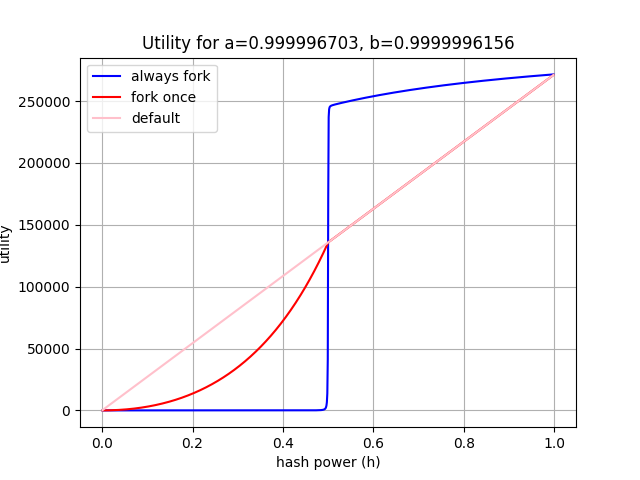
\includegraphics[width=0.46\textwidth]{plots/test_AF.png}
%    \caption{Utility for player $1$ under strategies $\bdf$, $\bpf{1}$ and $\baf$. The curve for $\bpf{1}$ is too close to that of $\df$ to tell a difference at this scale, but the difference does exist: after about $h = 0.5$, the curve for $\bpf{1}$ is always higher than that of $\df$. Note that the utility collapses to $\bdf$ when $h = 1$. This is always the highest amount that can be earned in our game.}
%        \label{fig-af-df-fo}
%\end{figure}
%
%\smallskip
%\noindent
%\francisco{I think the following subsection should not be included (or should be restated as only considering AF vs DF). The comparation with F[i] looks quite weak to me.}
%\textbf{Forking for a fixed number of times}. Looking at Figure \ref{fig-af-df-fo}, we see that the utility when using $\pf{1}$ is  between the lines for $\af$ and $\df$. 
%This utility was calculated using a similar strategy as in in the proof of Theorem \ref{thm:always_fork}. 
%From the figure one can infer that, assuming $\af$ yields more utility to player $1$ than $\df$ (e.g. when $h>0.5$), then player $1$ should not use $\pf{1}$ but rather keep on forking, as 
%the utility for $\af$ is always above than the utility for $\pf{i}$ in that case. %Can we say the same for other similar strategies? Even though we can compute the utility of using any of the strategies $\pf{i}$, we cannot directly compare an infinite number of strategies. Instead, we prove the following general result. 
%We can show something similar for all the other $\pf{i}$.
%\begin{proposition}\label{prop-fork_fix}
%Assume that $u_1(\bdf) \leq u_1(\baf)$ for some $\alpha,\beta,h$. Then for all $i > 0$ we have that $u_1((\df_0,\pf{i})) \leq u_1(\af))$.
%\end{proposition}
%
%Note that this result does not rule out the possibility that, for some amount of hash power, playing some $\pf{i}$ would turn out better than $\df$, but $\af$ would not. We know 
%this is not the case for $i = 1$, and we can also prove it for $i > 1$, albeit at the cost of much more powerful machinery that we do not have the space to introduce. 
%However, in the following section we do show that there are actually strategies leading to forks with less hash power. 

\subsection{Giving up for more utility}
\label{sec-giving-up}

%By adding a little more flexibility to the strategy of always forking, we can identify approaches that make a fork profitable with less hash power. The families of strategies that we study in this section involve two parameters. First, a \textit{give-up} parameter $\ell$ that mandates the maximum length of the fight the miner is willing to carry out when doing a fork, and a parameter $k$ that regulates how far back the miner is willing to do a fork, when confronted with a chain of blocks she does not own. We denote these strategies by $\gup_\ell^k$. 

By adding a little more flexibility to the strategy of always forking, we can identify approaches that make a fork profitable with less hash power. The families of strategies that we study in this section involve two parameters. The first parameter, denoted by $k$, regulates how far back the miner will fork, when confronted with a chain of blocks she does not own. The second parameter, called the \textit{give-up} time, and denoted by $\ell$, tells us the maximum number of blocks that the player's opponent is allowed to extend the current blockchain with before the player gives up mining on the forking branch. If the player does not manage to transform her fork into the new blockchain before her opponent mines more than $\ell$ blocks, she will restart the strategy treating the tail of the current blockchain as the new genesis block. We denote these strategies by $\gup_\ell^k$. 


\begin{figure}
\vspace{-15pt}
\centering
\begin{tikzpicture}[->,>=stealth',auto,thick, scale = 0.61,state/.style={circle,inner sep=2pt}]

    % The graph
	\node [state] at (-19.5,0) (aR) {$\varepsilon$};
	\node [state] at (-18,0) (a0) {$0$};
	\node [state] at (-16.5,0) (a00) {$00$};
	\node [state] at (-15,0) (a000) {$000$};
	\node [state] at (-18,-1.4) (aAF) {$\af$};
	\node [state] at (-16.5,-1.4) (aG) {$\gup_3^2$};
	\node [state] at (-21,-0.70) {(a)};

	% Graph edges
	\path[->]
	(aR) edge (a0)
	(a0) edge (a00)
	(a00) edge (a000);
  	
	\path[->,dashed]
	(aR) edge (aAF)
	(a0) edge (aG);
	
    % The graph
%	\node [state] at (-10.5,-2.8) (bR) {$\varepsilon$};
%	\node [state] at (-9,-2.8) (b0) {$0$};
%	\node [state] at (-7.5,-2.8) (b00) {$00$};
%	\node [state] at (-6,-2.8) (b000) {$000$};
%	\node [state] at (-4,-2.8) (b0000) {$0000$};
%	\node [state] at (-9,-4.3) (b1) {$1$};
%	\node [state] at (-7.5,-4.3) (b11) {$11$};
%	\node [state] at (-5.5,-4.3) (bAF) {$\af$};
%	\node [state] at (-1.5,-2.8) (bG) {$\gup_4^2$};
%	\node [state] at (-12,-3.70) {(b)};

	\node [state] at (-10.5,0) (bR) {$\varepsilon$};
	\node [state] at (-9,0) (b0) {$0$};
	\node [state] at (-7.5,0) (b00) {$00$};
	\node [state] at (-6,0) (b000) {$000$};
	\node [state] at (-4,0) (b0000) {$0000$};
	\node [state] at (-9,-1.4) (b1) {$1$};
	\node [state] at (-7.5,-1.4) (b11) {$11$};
	\node [state] at (-5.5,-1.4) (bAF) {$\af$};
	\node [state] at (-1.5,0) (bG) {$\gup_3^2$};
	\node [state] at (-12,-0.7) {(b)};
	
	% Graph edges
	\path[->]
	(bR) edge (b0)
	(bR) edge (b1)
	(b1) edge (b11)
	(b0) edge (b00)
	(b00) edge (b000)
	(b000) edge (b0000);
  	
	\path[->,dashed]
	(b11) edge (bAF)
	(b0000) edge (bG);
	

\end{tikzpicture} 
\vspace*{-25pt}
\caption{Difference between $\af$ and $\gup^2_3$ in terms of actions in two states. 
%In (a), the value $k = 2$ indicates that $\gup^2_4$ will not 
%fork on $\varepsilon$ but instead in $0$. In (b), the value $\ell = 4$ indicates that in this state player $1$ should give up the fork and continue mining upon the blockchain (block $0000$).
\label{fig-gup}}
\end{figure}




\begin{example}
Let us compare $\gup_3^2$ and $\af$. Since $k = 2$, both strategies take the same action when the state is $\{\varepsilon\}, \{\varepsilon,0\}$, and $\{\varepsilon,0,00\}$, namely, mining at $\varepsilon$. Hence, assume that both strategies are facing a chain of three 
%unowned new 
blocks owned by player 0, 
%in the blockchain, 
as shown in Figure \ref{fig-gup}(a). In this case, $\af$ would again try to do a fork from the genesis block as no block belongs to player~1. On the other hand, $\gup_3^2$ would try to  fork on the dotted line, that is, the second block that does not belong to her.
The second difference is provided by the give-up time, which is shown in Figure~\ref{fig-gup}(b). Normally, $\af$ is willing to continue forking regardless of the hope of winning, therefore the move for the state in Figure \ref{fig-gup}(b) would still be to mine upon her own block $11$. On the other hand, $\gup_3^2$ has now seen 4 blocks from the start of the fork (one more than the maximum $\ell = 3$), so with this strategy player $1$ instead gives up and tries to mine upon $0000$, rebooting the strategy as if 
%this last block 
$0000$ was the genesis block. Note also that $\af=\gup_\infty^\infty$. 
%, that is, the strategy where player $1$ is willing to keep fighting for a fork of any length, and to do a fork at the beginning of any chain of blocks she does not own.  \qed
\end{example}

\begin{figure*}

    \subfigure[Utilities for player 1 of combined strategies, $\bdf$, $\bgup^1_4$, $\bgup^1_5$ and $\baf$]{
        \begin{tikzpicture}
\begin{axis}[
    xmin=0,
    xmax=1,
    ymin=0,
    ymax=1,
    height=7cm,
    width=.7\linewidth,
    ylabel={Utility},
    ylabel near ticks,
    ytick=\empty,
    xtick={0,0.1,...,1},
    legend pos=north west,
]
\plotfile{plots/forking_strategies_data.csv}
\end{axis}
\end{tikzpicture}

        \label{fig-plot-gup-fixwindow}
    }
    \hfill
    \subfigure[Zoom in around the intersection%around the values of the hash power where $\bdf$ intersects with $\bgup^1_4$ and $\bgup^1_5$.
]{
        \begin{tikzpicture}{scale=1}
\begin{axis}[
    xmin=0.46,
    xmax=0.492,
    ymin=0.88,
    ymax=1,
    ytick=\empty,
    width=.37\linewidth,
    height=7cm,
    legend pos=north west,
    xtick={0.4675, 0.486},
    xticklabels={0.467, 0.486},
    grid=both,
]
\plotfilezoom{../plots/forking_strategies_zoom_data.csv}
\end{axis}
\end{tikzpicture}

        \label{fig-af-df-fo}
    }
\vspace*{-10pt}
    \caption{Comparing the utilities of three forking strategies against the default strategy}
    \label{fig-complex-strategies}
\end{figure*}

Define $\bgup_\ell^k$ as the combined strategy $(\df_0, \gup_\ell^k)$. We obtain an analytical form similar to that of Theorem \ref{thm:always_fork}, except in 
this case the set of paths leading to winning states has a more complex combinatorial nature, as expected when taking into account the 
%disadvantage and give-up 
parameters $k$ and $\ell$.
%To compute an analytical form for $u_1(\bgup_\ell^k)$, we proceed as in the proof of Theorem \ref{thm:always_fork}. In this case, the set of paths leading to winning states has a more complex combinatorial nature, as expected when taking into account the 
%disadvantage and give-up 
%parameters $k$ and $\ell$. We obtain the following.
\begin{theorem}\label{thm-dificil}
For every pair of positive integers $\ell, k$ with $k< \ell$, we have that:
$$u_1(\bgup^k_\ell) = \frac{\Phi_{\ell,k}}{1-\Gamma_{\ell,k}},$$
where $\Phi_{\ell,k}$ and $\Gamma_{\ell,k}$ are rational functions of $\alpha$, $\beta$ and $h$.% (that is, divisions of polynomials of  $\alpha$, $\beta$ and $h$).
\end{theorem}
In the proof of this theorem we develop precise expressions for $\Phi_{\ell, k},\Gamma_{\ell,k}$.  %(appendix \ref{sec-evaluation-G}),
They involve two sets
of polynomials related to Dyck words, which describe the combinatorial nature of
the game. %In what follows we give a sketch of the proof of this theorem. The complete proof is given in appendix \ref{sec-evaluation-G}.

\begin{comment}
\medskip

{\sc Proof sketch.} Consider the beginning of the game, where both players are
mining on $\varepsilon$ and there are no other blocks. From this point, and
until both players are mining again on a common block, five scenarios can
arise. In the first case, miner 1 (playing with $G_\ell^k$) immediately appends
a block $b$ on top of $\varepsilon$, after which both players will mine on top
of $b$ (as dictated by their strategies).  The second and third cases are those
in which which miner 0 appends $j\leq k$ blocks on top of $\varepsilon$ and
miner 1 appends another block on $\varepsilon$, eventually winning the fork
(case 2) or giving up (case 3), and again, after this point both strategies
will dictate to mine on top of the same block. The last two cases occur when
miner 0 appends $j>k$ blocks on top of $\varepsilon$, after which miner 1
manages to append a block at position $j-k$, starting a fork and eventually
winning (case 4) or again giving up (case 5).  These five cases partition the space
of possible states with positive reward for miner 1, which 
can then be analysed separately using combinatorial computations. After any of the
states discussed above, both players mine on the same block and, therefore, the
strategies advise similar actions as in the beginning of the game. 
%(this happens because of the way these strategies are defined).  
Thus, as in the case of
Theorem
\ref{thm:always_fork}, we have an equation of the form $u_1(\bgup^k_\ell)  =
\Phi_{\ell, k}+\Gamma_{\ell, k}\cdot u_1(\bgup^k_\ell)$, where $\Phi_{\ell, k}$
is the utility contribution of the set of the above finite states and
$\Gamma_{\ell, k}$ is a proper shifting factor.  
Once again, an important combinatorial challenge of this proof is to quantify the number of different 
paths leading to states in which both players mine the same block. 
We represent them as 
%In order to obtain expressions
%for these quantities, we represent states as 
unitary north-east paths
inside polygons in $\ZZ^2$, where north and east steps represent blocks
appended by miner 0 and miner 1, respectively.  
To count these paths we provide the following combinatorial result. 
\begin{lemma} For nonnegative
    integers $a,b$, let $\sigma_{a,b}$ be the amount of one-step north-east
    paths from $(0,0)$ to $(a+b,b)$ that stay inside of the trapezoid
    $\{(0,0),(a,0),(0,b),(a+b,b)\}.$ We have that
\begin{eqnarray*}
\sigma_{a,b} & = & \frac{(a+b)\cdot(a+2b)!}{b!\cdot(a+b+1)!}=\frac{a+1}{a+b+1}\cdot {a+2b\choose a+b}.
\end{eqnarray*}
    Also, for nonnegative integers $a,b,r$ such that $r>a$, let $\theta_{a,b}^r$ be the
 amount of such paths from $(0,0)$ to $(r,b)$ that do not exit the pentagon
 $\{(0,0),(a,0),(r,r-a),(r,b),(0,b)\}$. Then we have the following:
 $$
\theta_{a,b}^r = \displaystyle \sigma_{|b-r|,\min(r,b)} + \sum_{i=\max(1,r-b+1)}^a  \bigg(\sum_{j=0}^{r-i}\sigma_{i-1,j}\cdot \sigma_{i+b-r,r-i-j} \bigg).
 $$
 \end{lemma}
 For the proof, we write the utility as given in Definition \ref{def-utility}, separate the summation 
 over the five cases explained above, and then show that these sums can be expressed in terms of the 
 generating polynomials associated to the sequences $\sigma_{a,b}$ and $\theta_{a,b}^r$, which we
refer to as \textit{Trapezoidal and Pentagonal Dyck polynomials}.
%After writing the utility in this case, as given in definition \ref{def-utility},
%and separating the summation over the set of states into these five cases, the
%result is given as a combination of the generating polynomials associated to
%these sequences, which we
%refer to as \textit{Trapezoidal and Pentagonal Dyck polynomials}, completing the
%proof. 
\qed

\medskip
\end{comment}

%In other words, given specific values of $k$ and $\ell$, we can still compute the utility of these strategies.
We use Theorem \ref{thm-dificil} to analyse these strategies, plotting them, as we did before, 
for $\alpha = 0.9999966993$ and $\beta = 0.9999996156$. Figures  \ref{fig-plot-gup-fixwindow} and \ref{fig-af-df-fo} give 
%us an 
interesting 
%feel 
information about the advantages of these strategies. 
We fix $k = 1$, and plot in Figure \ref{fig-plot-gup-fixwindow} the utilities of combined strategies $\bdf$, $\bgup^1_4$, $\bgup^1_5$ and $\baf$. In Figure \ref{fig-af-df-fo}, we zoom in around the values of the hash power where $\bdf$ intersects with $\bgup^1_4$ and $\bgup^1_5$.
%, and shade those areas in which one of the utilities is greater. 
As we see in the figures, for a 
fork window $k = 1$, the optimal amount time player $1$ should be willing to fight for a branch before giving up depends on the hash power. With little hash power the likelihood of winning a 
branch is small, so player 1 should give up as early as possible. However, the more hash power she obtains, the better it is to wait more. Interestingly, with more than 
$46.7\%$ of the hash power, player $1$ already should start using strategy $\gup^1_4$ to defeat the default strategy, and with more than $48.6\%$ hash power, she should adopt $\gup^1_5$. We know that player~$1$ should use $\af$ not before around $h = 0.499805$, so this gives us a lot of extra room to look for optimal strategies if we are willing to fork (especially considering that every percentage of hash power in popular cryptocurrencies 
may cost millions).

Plots for strategies with $k > 1$ present a similar behaviour: the more hash power we have, the more we should be willing to fight for our forks. The strategies we include 
in Figure \ref{fig-complex-strategies} beat the default strategy under the least amount of hash power 
amongst any combination of values for $k$ and $\ell$ with $k < \ell \leq 100$. The comparison is much less straightforward when looking at varying values of both $k$ and $\ell$, but in general, 
the more hash power the bigger the window of blocks one should aim to do a fork, and the more one should wait before giving up. 

%The analysis we can do  through 2- or 3-dimensional plots is only one part of the picture, and a game-theoretical analysis of these strategies is an interesting area for future work. 
%Furthermore, the techniques used to prove theorems \ref{thm:always_fork} and \ref{thm-dificil} can be in fact generalised for any pair of strategies satisfying arguably natural conditions: There is always a point in the future in which both players mine upon the last block of the blockchain, and the corresponding state can be treated as if it was $\varepsilon$ (after proper shifting).


%%%%%%%%%%%%%%%%%%%%%%%%%%%%%%%%%%%%%%%%%%%%%%%%%%%%%%%%%%%%%%%%%%%%%%%%%
%%% BELOW IS THE PREVIOUS VERSION THAT I STILL DID NOT MAKE A PASS ON %%%
%%%%%%%%%%%%%%%%%%%%%%%%%%%%%%%%%%%%%%%%%%%%%%%%%%%%%%%%%%%%%%%%%%%%%%%%%

\begin{comment}

\paragraph{Forking in the genesis block.}
The first forking strategy we models the case when 0 has won the ultimate block. The question 1 wants to answer in this situation is whether she should continue mining on the blockchain, playing according to $\df$, or should she fork, mining instead upon her previously won block? Since by the proof of Theorem \ref{thm-conts_equlibria} we know that optimal strategies for 1 depend only on the blocks following her last block in each state, we can focus on this question when the game is just starting, that is, when 1 wants to decide whether to fork in the genesis block. We will denote by $\fg_1$ the strategy in which player 1 is trying to win the first block following genesis, and once this branch becomes the new blockchain, continues mining using the default strategy. We denote by $\fg = (\df_0,\fg_1)$ the strategy where 1 tries to win the first block in the final blockchain, and 0 mines using the default strategy. A depiction of this strategy is given in Figure \ref{fig-fork_genesis}. When player 1 uses this strategy, we can compute her utility as follows.

\begin{figure}
\begin{center}
\begin{tikzpicture}[->,>=stealth',auto,thick, scale = 1.0,state/.style={circle,inner sep=2pt}]

    % The graph
	\node [state] at (0,0) (R) {$\varepsilon$};
	\node [state] at (1.5,0.75) (1) {$1$};
	\node [state] at (1.5,-0.75) (0) {$0$};
	\node [state] at (3,-0.75) (00) {$00$};
	
	\node [state] at (3,0.75) (11) {$11$};		
	\node [state] at (4.6,0.75) (111) {$111$};
	\node [state] at (6.4,0.75) (1110) {$1110$};
			

	
	% Graph edges
	\path[->]
	(R) edge (1)
	(R) edge (0)
	(0) edge (00)
	;  	
	
	\path[->,dashed]
	(1) edge (11)
	(11) edge (111)
	(111) edge (1110)
	;


\end{tikzpicture} 
\end{center}
\caption{Following the block 00 player 1 tries to win a fork starting at $\varepsilon$. Dashed edges show the case in which she succeeds, after which both players mine on top of the new blockchain.}
\label{fig-fork_genesis}
\end{figure}

\begin{myprop}
%	\label{prop-utilityofgenesisinfinite}
	\label{prop:utility_gen_fork}
%	Suppose player 1 plays with the genesis fork strategy and player 0 follows the default strategy. 
Let $h$ be the hash power of player 1. Then
	\begin{eqnarray*}
		u_1^\infty(\fg\mid\varepsilon) =K_1\cdot \Cat(\beta^2h(1-h))+K_2\cdot \Cat(\alpha\beta^2h(1-h))
	\end{eqnarray*}
where $\Cat:x\mapsto \frac{1-\sqrt{1-4x}}{2x}$ is the generating function of Catalan numbers \cite{ADD_CITATION}, and 
	\begin{eqnarray*}
		K_1 =\frac{\alpha\beta h}{(1-\alpha)(1-\beta)},\quad	K_2 =\frac{\alpha^2\beta h(\alpha\beta+h\beta-h\alpha\beta-1)}{(1-\alpha)(1-\beta)(1-\alpha\beta)}.	
	\end{eqnarray*}
\end{myprop}

The intuition behind the appearance of Catalan numbers in this result is that for each fixed $n$, the number of states where two chains of length $n$ are being tied for blockchain equals the $n$th Catalan number (more precisely, they correspond to Dyck paths of length $n$). Since such states dictate when 1 will win the desired fork, and no reward can be won by 1 before this occurs (note that the two branches in this game have only $\varepsilon$ in common), they tell us what the utility of player 1 will be. Notice that since $\beta \leq 1$, and the maximum of the function $h\mapsto h(1-h)$ is $\frac{1}{4}$, for $h\in [0,1]$, the value $Cat(\beta^2h(1-h))$ is always well defined. For the sake of completion, in Appendix \ref{appendix-gen_fork}, we also show what is the utility of $\fg$ for player 1 at each step $n$ of the mining game.

\paragraph{Forking $m$ blocks from the end of the blockchain.} The second forking strategy we consider works similarly as $\fg$, but now player 1 considers forking after losing $m$ consecutive blocks, for some fixed $m$. In this case, 1 will fork $m$ blocks from the end of the current blockchain, all of these $m$ block being owned by 0. This situation is depicted in Figure \ref{fig-fork_m}. Once player 1 wins the fork, and this branch becomes the new blockchain, she will continue mining according to $\df_1$. We denote this strategy of player 1 by $\forkm{m}_1$, and denote with $\forkm{m}=(\df_0,\forkm{m}_1)$ the strategy where 1 uses $\forkm{m}_1$, and 0 plays according to the default strategy.

\begin{figure}
\begin{center}
\begin{tikzpicture}[->,>=stealth',auto,thick, scale = 1.0,state/.style={circle,inner sep=2pt}]

    % The graph
	\node [state] at (0,0) (R) {$\varepsilon$};
	\node [state] at (1.5,0) (0) {$0$};
	\node [state] at (3,0) (01) {$01$};
	\node [state] at (4.6,0) (010) {$010$};
	\node [state] at (6.4,0) (0100) {$0100$};
	
	\node [state] at (4.6,0.75) (011) {$011$};					
	
	% Graph edges
	\path[->]
	(R) edge (0)
	(0) edge (01)
	(01) edge (010)
	(010) edge (0100)	
	;  	
	
	\path[->,dashed]
	(01) edge (011)
	;


\end{tikzpicture} 
\end{center}
\caption{If playing $\forkm{2}_1$, player 1 will try to fork after losing two consecutive blocks at position 0100. Should she manage to make the dashed branch into a blockchain, both her and player 1 continue to mine on this branch using $\df$.}
\label{fig-fork_m}
\end{figure}

When computing the utility of $\forkm{m}$ starting in some state $q_0$, we take into account that player 1 is only interested whether her utility will increase in the case she decides to fork. That is, since the blocks before her fork will always have the same constant contribution to her reward in either branch, we will not count them in the utility. With this in mind, the utility of $\forkm{m}$ starting in the state $q_0$ in which 0 has the ultimate $m$ blocks in the (up to now unique) blockchain is given as follows.

\begin{myprop}\label{prop-fork_m}
	Let $h$ be the hash power of player 1. Then
	\begin{eqnarray*}
		u_1(\mfork|q_0) =\bigg(\frac{\beta h}{\alpha}\bigg)^m K_{1}\Cat(\beta^2h(1-h))^{m+1}+(\beta h)^{m}K_{2}\Cat(\alpha\beta^2h(1-h))^{m+1}
	\end{eqnarray*}
	where $\Cat$ is as in Proposition \ref{prop:utility_gen_fork}, and 

\end{myprop}

As before, Catalan numbers help us account for all states where 1 wins the fork. Of course, now player 1 is starting with a handicap of $m$ steps, so the winning states for 1 will be characterized by staircase walks that stay inside the trapezoid $\{(0,0),(m,0),(m+n,n),(0,n)\}$, for some number $n$. The proof of this proposition is given in Appendix \ref{appendix-fork_m}.

\paragraph{When to fork?} Having the utilities of the two forking strategies, we can now compare them to that of the default strategy in order to answer whether 1 should fork or not. Analysing the curves defined by the game parameters ($\alpha,\beta$ and $h$ for $\fg$, and additionally $m$ for $\forkm{m}$), it can be seen that when $h>50\%$, and $\alpha>\beta$, then it is always convenient for 1 to fork, based on the utility resulting from either $\fg$ or (irrespective of $m$) $\forkm{m}$. This confirms the intuition that the player with the majority of hash power can sway the game in her favour, but we can also see that there are several cases when it is convenient to fork even with much lower hash power. This happens in cases when $\alpha$ is significantly bigger than $\beta$, which can be explained by the fact that ???

\end{comment}

\section{Concluding remarks}
\label{sec-con-r}

Our model of mining via a stochastic game allows for an intuitive representation of miners' actions as strategies, 
and gives us a way of understanding the rational behaviour of miners looking to accumulate cryptocurrency wealth. 
In this respect, we would like to identify strategies that are a nash equilibrium for the case of decreasing rewards. However, this has proven 
to be a difficult task. For starters, in the two player game one can show that the default strategy can never be part of such an 
equilibrium, no matter how small the hash power is for one of the players. This means that one must look for much more complex strategies if one 
wants to find such an equilibrium. 

One of the advantages of our model is its generality: it can be adapted to specify more complex 
actions, study other forms of reward and include cooperation between miners. 
We are currently looking at strategies that involve withholding 
a mined block to the rest of the network, for which we need a slight extension of the notions of action and state. 
We would also like to study incentives under different models of cooperation between miners, and 
also other forms of equilibria in a dynamic setting. 



\bibliographystyle{ACM-Reference-Format}
\bibliography{../extras/bibliography}

\newpage
\onecolumn
\appendix
%!TEX root = main.tex

\section{Proofs and Intermediate Results}
\subsection{Convergence of the utility function}
\label{sec-conver}

To ensure that the utility function $u_p(\bs \mid q_0)$ is well defined, we impose the restriction that for every payoff function $\bR = (r_0, \ldots, r_{m-1})$, there exists a polynomial $P$ such that $|r_p(q)| \leq P(|q|)$ for every player $p \in \bP$ and state $q \in \bQ$. In this section, we prove that this is indeed a sufficient condition for $u_p(\bs \mid q_0)$ to be a real number, for which we first need a technical lemma. 

\begin{mylem}\label{lem-prop-k}
Let $q_0 \in \bQ$ and $\bs$ be a combined strategy. Then for every $k \geq 0$, it holds that
\begin{eqnarray*}
\sum_{\substack{q \in \bQ \,: \\ q_0 \subseteq q \text{ {\rm and} } |q| - |q_0| = k}} \pr^{\bs}(q \mid q_0) & = & 1.
\end{eqnarray*}
\end{mylem}

\begin{proof}
We prove the lemma by induction on $k$. For $k=0$ the property trivially holds since $\pr^{\bs}(q_0 \mid q_0) = 1$. Thus, assuming that the property holds for $k$, we need to prove that it holds for $k+1$. We have that:
\begin{align*}
&\sum_{\substack{q \in \bQ \,: \\ q_0 \subseteq q \text{ {\rm and} } |q| - |q_0| = k+1}} \pr^{\bs}(q \mid q_0) \ =\\
&\hspace{30pt}\sum_{\substack{q \in \bQ \,: \\ q_0 \subseteq q \text{ {\rm and} } |q| - |q_0| = k+1}} 
\bigg(\sum_{\substack{q' \in \bQ \,: \\ q_0 \subseteq q' \text{ {\rm and} } |q'| - |q_0| = k}} \pr^{\bs}(q' \mid q_0) \cdot \pr(q',\bs(q'),q)\bigg) \ = \\
&\hspace{30pt}\sum_{\substack{q' \in \bQ \,: \\ q_0 \subseteq q' \text{ {\rm and} } |q'| - |q_0| = k}}
\bigg(\sum_{\substack{q \in \bQ \,: \\ q_0 \subseteq q \text{ {\rm and} } |q| - |q_0| = k+1}} 
 \pr^{\bs}(q' \mid q_0) \cdot \pr(q',\bs(q'),q)\bigg) \ =\\
 &\hspace{30pt}\sum_{\substack{q' \in \bQ \,: \\ q_0 \subseteq q' \text{ {\rm and} } |q'| - |q_0| = k}}
\pr^{\bs}(q' \mid q_0) \cdot \bigg(\sum_{\substack{q \in \bQ \,: \\ q_0 \subseteq q \text{ {\rm and} } |q| - |q_0| = k+1}} 
  \pr(q',\bs(q'),q)\bigg) \ =\\
&\hspace{30pt}\sum_{\substack{q' \in \bQ \,: \\ q_0 \subseteq q' \text{ {\rm and} } |q'| - |q_0| = k}}
\pr^{\bs}(q' \mid q_0) \cdot \bigg(\sum_{\substack{q \in \bQ \,: \\ q_0 \subseteq q,\ |q| - |q_0| = k+1,\ \bs(q') = (a_0, \ldots, a_{m-1}) \text{ {\rm and}}\\
\text{{\rm there exists }} p \in \{0, \ldots, m-1\} \text{ {\rm such that} } q = a_p(q')}}
  \pr(q',\bs(q'),q)\bigg) \ =\\
  &\hspace{30pt}\sum_{\substack{q' \in \bQ \,: \\ q_0 \subseteq q' \text{ {\rm and} } |q'| - |q_0| = k}}
\pr^{\bs}(q' \mid q_0) \cdot \bigg(\sum_{\substack{p \in \{0, \ldots, m-1\} \, : \\ \bs(q) = (a_0, \ldots, a_{m-1})}} \pr(q',\bs(q'),a_p(q'))\bigg) \ =\\
&\hspace{30pt}\sum_{\substack{q' \in \bQ \,: \\ q_0 \subseteq q' \text{ {\rm and} } |q'| - |q_0| = k}}
\pr^{\bs}(q' \mid q_0).
\end{align*}
Hence, given that
\begin{eqnarray*}
\sum_{\substack{q' \in \bQ \,: \\ q_0 \subseteq q' \text{ {\rm and} } |q'| - |q_0| = k}}
\pr^{\bs}(q' \mid q_0) & = & 1
\end{eqnarray*}
by induction hypothesis, we conclude that
\begin{eqnarray*}
\sum_{\substack{q \in \bQ \,: \\ q_0 \subseteq q \text{ {\rm and} } |q| - |q_0| = k+1}}
\pr^{\bs}(q \mid q_0) & = & 1.
\end{eqnarray*}
\end{proof}

\begin{myprop}\label{prop-conv}
Let $p \in \{0, \ldots, m-1\}$, $q_0 \in \bQ$ and $\bs$ be a combined strategy. If there exist a polynomial $P$ such that $|r_p(q)| \leq P(|q|)$ for every $q \in \bQ$, then $u_p(\bs \mid q_0)$ is a real number.
\end{myprop}

\begin{proof}
Notice that if $P$ is a zero polynomial, then the property trivially holds. Thus, we assume that $P$ is a nonzero polynomial. 
Then we have that:
\begin{eqnarray}
\notag
u_p(\bs \mid q_0) & =  & (1-\beta) \cdot \sum_{q \in \bQ \,:\, q_0 \subseteq q} \beta^{|q|-|q_0|} \cdot  r_p(q) \cdot \pr^{\bs}(q \mid q_0)\\
\notag
& = & (1-\beta) \cdot \sum_{n=0}^\infty \bigg(\sum_{\substack{q \in \bQ \,: \\ q_0 \subseteq q \text{ {\rm and} } |q| - |q_0| = n}} \beta^{|q|-|q_0|} \cdot  r_p(q) \cdot \pr^{\bs}(q \mid q_0)\bigg)\\
\label{eq-gen-form}
& = & (1-\beta) \cdot \sum_{n=0}^\infty \beta^n \cdot \bigg(\sum_{\substack{q \in \bQ \,: \\ q_0 \subseteq q \text{ {\rm and} } |q| - |q_0| = n}} r_p(q) \cdot \pr^{\bs}(q \mid q_0)\bigg).
\end{eqnarray}
Let $f : \mathbb{N} \to \mathbb{R}$ be a function defined as:
\begin{eqnarray*}
f(n) & = & \sum_{\substack{q \in \bQ \,: \\ q_0 \subseteq q \text{ {\rm and} } |q| - |q_0| = n}} r_p(q) \cdot \pr^{\bs}(q \mid q_0).
\end{eqnarray*}
Notice that this function is well-defined as there exists a finite number of states $q \in \bQ$ such that $|q| - |q_0| = n$. Then by equation \eqref{eq-gen-form}, we have that:
\begin{eqnarray*}
u_p(\bs \mid q_0) & = & (1-\beta) \cdot \sum_{n=0}^\infty \beta^n \cdot f(n).
\end{eqnarray*}
Therefore, to show that $u_p(\bs \mid q_0)$ is a real number, we need to show that the series $ \sum_{n=0}^\infty \beta^n \cdot f(n)$ converges, for which we prove that the series $ \sum_{n=0}^\infty |\beta^n \cdot f(n)|$ converges (that is, we show that $ \sum_{n=0}^\infty \beta^n \cdot f(n)$ converges absolutely, which is known to imply that this series is convergent). By definition of function $f$, we have that:
\begin{eqnarray}
\notag
|f(n)| & = & \bigg| \sum_{\substack{q \in \bQ \,: \\ q_0 \subseteq q \text{ {\rm and} } |q| - |q_0| = n}} r_p(q) \cdot \pr^{\bs}(q \mid q_0) \bigg|\\
\notag
& \leq & \sum_{\substack{q \in \bQ \,: \\ q_0 \subseteq q \text{ {\rm and} } |q| - |q_0| = n}} |r_p(q)| \cdot \pr^{\bs}(q \mid q_0)\\
\notag
& \leq & \sum_{\substack{q \in \bQ \,: \\ q_0 \subseteq q \text{ {\rm and} } |q| - |q_0| = n}} P(n) \cdot \pr^{\bs}(q \mid q_0)\\
\label{eq-f-abs}
& = & P(n) \cdot \bigg(\sum_{\substack{q \in \bQ \,: \\ q_0 \subseteq q \text{ {\rm and} } |q| - |q_0| = n}} \pr^{\bs}(q \mid q_0)\bigg).
\end{eqnarray}
We have by Lemma \ref{lem-prop-k} that
\begin{eqnarray*}
\sum_{\substack{q \in \bQ \,: \\ q_0 \subseteq q \text{ {\rm and} } |q| - |q_0| = n}} \pr^{\bs}(q \mid q_0) & = & 1.
\end{eqnarray*}
Hence, we conclude by equation \eqref{eq-f-abs} that:
\begin{eqnarray*}
|f(n)| & \leq & P(n).
\end{eqnarray*}
Thus, we have that:
\begin{eqnarray}\label{eq-bound-p}
\sum_{n=0}^\infty |\beta^n \cdot f(n)| \ = \ \sum_{n=0}^\infty \beta^n \cdot |f(n)|
\ \leq \ \sum_{n=0}^\infty \beta^n \cdot P(n).
\end{eqnarray}
Given that every term in the series $\sum_{n=0}^\infty |\beta^n \cdot f(n)|$ is non-negative, to show that this series converges it is enough to prove that it is bound by a (non-negative) real number. Thus, by equation \eqref{eq-bound-p}, to finish the proof we need to show that the series $\sum_{n=0}^\infty \beta^n \cdot P(n)$ converges. By this can be easily established by using the Ratio Test, as we have that $\beta \in (0,1)$ and
\begin{eqnarray*}
\lim_{n \to \infty} \frac{\beta^{n+1} \cdot P(n+1)}{\beta^{n} \cdot P(n)} \ = \ \beta \cdot \lim_{n \to \infty} \frac{P(n+1)}{P(n)}
\ = \ \beta,
\end{eqnarray*}
since $\lim_{n \to \infty} \frac{P(n+1)}{P(n)} = 1$ as $P$ is a nonzero polynomial.
This concludes the proof of the proposition.
\end{proof}

\subsection{Proof of Proposition \ref{prop-ub-block}}
We have that:
\begin{eqnarray*}
u_p(\bs ) & =  & (1 - \beta) \cdot  \sum_{q \in \bQ \,:\, b \in q} \beta^{|q|-1} \cdot  r_p(b,q) \cdot \pr^{\bs}(q )\\
& \leq & (1 - \beta) \cdot  \sum_{q \in \bQ \,:\, b \in q} \beta^{|q|-1} \cdot  M_p(b) \cdot \pr^{\bs}(q )\\
& = & (1 - \beta) \cdot  M_p(b) \cdot \sum_{q \in \bQ \,:\, b \in q} \beta^{|q|-1} \cdot   \pr^{\bs}(q )\\
& = & (1 - \beta) \cdot  M_p(b) \cdot \sum_{i=|b|+1}^\infty \bigg(\sum_{q \in \bQ \,:\, b \in q \text{ and } |q| = i} \beta^{|q|-1} \cdot   \pr^{\bs}(q )\bigg)\\
& = & (1 - \beta) \cdot  M_p(b) \cdot \sum_{i=|b|+1}^\infty \bigg(\beta^{i-1} \cdot \sum_{q \in \bQ \,:\, b \in q \text{ and } |q| = i} \pr^{\bs}(q )\bigg)\\
& \leq & (1 - \beta) \cdot  M_p(b) \cdot \sum_{i=|b|+1}^\infty \bigg(\beta^{i-1} \cdot \sum_{q \in \bQ \,:\, |q| = i} \pr^{\bs}(q )\bigg).
\end{eqnarray*}
By lemma \ref{lem-prop-k}, we have that $\sum_{q \in \bQ \,:\, |q| = i} \pr^{\bs}(q ) = 1$. Hence, we conclude that:
\begin{eqnarray*}
u_p(\bs ) & \leq & (1 - \beta) \cdot  M_p(b) \cdot \sum_{i=|b|+1}^\infty \bigg(\beta^{i-1} \cdot \sum_{q \in \bQ \,:\, |q| = i} \pr^{\bs}(q )\bigg)\\
& = & (1 - \beta) \cdot  M_p(b) \cdot \sum_{i=|b|+1}^\infty \beta^{i-1}\\
& = & (1 - \beta) \cdot  \beta^{|b|} \cdot M_p(b) \cdot  \sum_{i=|b|+1}^\infty \beta^{i-1-|b|}\\
& = & (1 - \beta) \cdot  \beta^{|b|} \cdot M_p(b) \cdot \sum_{j=0}^\infty \beta^{j}\\
& = & (1 - \beta) \cdot  \beta^{|b|} \cdot M_p(b) \cdot \frac{1}{1-\beta}\\
& = & \beta^{|b|} \cdot M_p(b), 
\end{eqnarray*}
which was to be shown. 

\subsection*{Proof of Claim \ref{claim-nonempty-inter-gen}}

For the sake of contradiction, assume that
%Assume for contradiction two different  states 
$q,q'$ are two distinct states in $Q_{\bs}$ such that both $\sigma(q)$ and $\sigma(q')$ contain a state $q^* \in Q_\cdf$. By definition of $Q_\cdf$, there exists a block 
%$w$ 
$b^*$ such that $q^* = \{b \in \bB \mid b \preceq b^*\}$.
% is the closure (over prefixes) of $w$. 
By definition of mapping $\sigma$, there exist a sequence $\rho = q_0,\dots,q_n$ for $q$ and a sequence $\rho' = q_0',\dots,q_n'$ for $q'$ such that $b^* = b_\rho$ and $b^* = b_{\rho'}$. If 
$\rho = \rho'$, then $q = q'$ as $q = q_n$ and $q' = q'_n$. Hence, we have that $\rho \neq \rho'$.
%, so $\rho$ must be different from $\rho'$. 
Let $i$ be the first position where $\rho$ and $\rho'$ differ,
%are different, 
so that 
sequences $q_0,\dots,q_{i-1}$ and $q_0,\dots,q'_{i-1}$ are the same and $q_i \neq q_i'$ (notice that $i \in \{1, \ldots, n\}$ since $q_0 = q'_0 = \varepsilon$).
%except for the last state. 
Then both $q_i$ and $q_i'$ are reachable from $q_{i-1}$ in one step. Therefore, it follows that 
%by the construction of our game 
$q_i = a_{p_1}(q_{i-1})$ and $q'_i = a_{p_2}(q_{i-1})$, where $a_{p_1} = s_{p_1}(q_{i-1})$, $a_{p_2} = s_{p_2}(q_{i-1})$ and $p_1 \neq p_2$. Hence, we have that the symbols in the $i$-th positions of $b_\rho$ and $b_{\rho'}$ are different, from which we conclude that $b_\rho \neq b_{\rho'}$, and reach a contradiction since $b^* = b_\rho$ and $b^* = b_{\rho'}$.
%is different from the symbol in the $
%the word generated from $\pi$ and $\pi'$ is not the same. 


\subsection*{Proof of Lemma \ref{lem:default_utility}}
By the definition of utility we have:
\begin{eqnarray*}
u_1(\bdf) & = & (1-\beta) \cdot \sum_{q\in \bQ}\beta^{|q|-1}\cdot r(q)\cdot \pr^{\bdf}(q).
\end{eqnarray*}
Separating the sum by the state size, we can write:
\begin{eqnarray*}
u_1(\cdf) & = & (1-\beta) \cdot \sum_{i=1}^{\infty}\beta^{i-1} \cdot  \bigg(\sum_{\substack{q \in \bQ \,: |q| = i}} r_1(q) \cdot 
\pr^{\cdf}(q)\bigg).
\end{eqnarray*}
By encoding each state $q\in\bQ$ as a binary string $w\in \bstring$ (as in the proof of Theorem \ref{thm:always_fork} ) we can compute the utility as follows:
\begin{eqnarray*}
u_1(\cdf)& = & (1-\beta) \cdot c\cdot \sum_{i=0}^{\infty}\beta^{i} \cdot\bigg(\sum_{w\in\{0,1\}^i}  \bigg( \sum_{j=1}^{i}w[j] \cdot \alpha^j \bigg)\cdot 
\pr^{\cdf}(q_w)\bigg),
\end{eqnarray*}
where $w[j]$ is the $j$-th symbol of the string $w$ and $q_w = \{ b \in \bB \mid b \preceq w\}$. 
Notice that in the equation above, we use the fact that when playing $\cdf$ each state contains a single blockchain (and nothing else), thus implying that for every word $w\in \{0,1\}^*$, it holds that $\meet(q_w) = \bchain(q_w)$ and $\chi_1(b) = \owner(b) = w[j]$, for every block $b \in q_w$ such that $|b| = j \geq 1$. By rearranging the order of the summation we obtain:
\begin{eqnarray*}
u_1(\cdf )& = &(1-\beta) \cdot c\cdot \sum_{i=0}^{\infty}\beta^{i} \cdot \bigg(\sum_{j=1}^{i} \alpha^j \cdot\bigg(\sum_{w\in\{0,1\}^i}   w[j]\cdot 
\pr^{\cdf}(q_w)\bigg)\bigg)
\end{eqnarray*}
Using the fact that that mining any block for player 1 is an independent Bernoulli trial with probability of success $h$, and the fact that $\pr^{\cdf}(\{q_w \mid w\in \{0,1\}^i \text{ and } w[j]=1\})=h$ and $\pr^{\cdf}(\{q_w \mid w\in \{0,1\}^i \text{ and } w[j]=0\})=(1-h)$, for all $i \geq 1$ and $j \in \{1, \ldots, i\}$, we can conclude that $\sum_{w\in\{0,1\}^i}   w[j] \cdot \pr^{\cdf}(q_w) = \expected(w[j]) = h$, thus yielding:
\begin{eqnarray*}	
u_1(\cdf) \ = \ (1-\beta) \cdot c\cdot \sum_{i=0}^{\infty}\beta^{i} \cdot \bigg(\sum_{j=1}^{i} \alpha^j \cdot \expected(w[j])\bigg) \ = \ (1-\beta) \cdot c \cdot h \cdot \sum_{i=0}^{\infty}\beta^{i} \cdot \bigg(\sum_{j=1}^{i} \alpha^j\bigg) .
\end{eqnarray*}
Computing the final summation, we get:
\begin{eqnarray*}	
u_1(\cdf) & = & (1-\beta) \cdot c \cdot h\cdot \sum_{i=0}^{\infty}\beta^{i} \cdot \frac{\alpha\cdot (1-\alpha^i)}{1-\alpha}\\
 & = & (1-\beta) \cdot c \cdot h\cdot \frac{\alpha}{1-\alpha} \cdot \bigg(\sum_{i=0}^{\infty}\beta^{i} - \sum_{i=0}^{\infty}(\alpha \cdot \beta)^i \bigg).
\end{eqnarray*}
Using the fact that $\sum_{i=0}^{\infty}x^i= \frac{1}{1-x}$ for $x \in (0,1)$, we obtain the desired result:
\begin{eqnarray*}
u_1(\cdf) & = & h\cdot c\cdot\frac{\alpha\cdot\beta}{(1-\alpha\cdot\beta)}.
\end{eqnarray*}

\subsection{Proof of Theorem \ref{thm:always_fork}}
Let $Q_\baf = \{q \in \bQ \mid \pr^\baf(q) > 0\}$ be the set of all states that can be reached from the genesis block using the strategy $\baf$, and from the proof of Theorem \ref{thm-conts_dom_str} recall the definition of sequence $\rho$ for a state $q$, and recall the construction of string $b_\rho$ from such a sequence $\rho$.
%the mapping $\sigma: Q_\baf \rightarrow 2^{\bQ_\bdf}$ introduced  in the proof of Theorem \ref{thm-conts_dom_str}, now in the context of strategy $\baf$. From the function $\sigma$, we define $\tau:Q_\baf \mapsto 2^{\{0,1\}^*}$ as follows:
By using these elements, we define $\tau:Q_\baf \mapsto 2^{\{0,1\}^*}$ as follows:
\begin{eqnarray*}
\tau(q) & = & \{ b_\rho \mid \rho \text{ is a sequence for } q\}.
\end{eqnarray*}
Intuitively, $\tau(q)$ is the set of all moves that players 0 and 1 can do in $|q|-1$ steps according to $\baf$ that lead them to the state $q$ when starting in the genesis block. As such, they are coded as sequences of zeros and ones that tell us which player puts a block at the stage $i$ of the game, for $i \in \{ 1,\ldots, |q|-1\}$. It is straightforward to verify the following:
\begin{myclaim}\label{claim-words-app} For every $q, q'\in Q_\baf$, it holds that:
\begin{itemize}
\item[(a)] If $q\neq q'$, then $\tau(q)$ is disjoint from $\tau(q')$.
\item[(b)] $\pr^{\baf}(q) = \sum_{w \in \tau(q)} \pr(w)$, where $\pr(w)$ for a word $w$ with $n_0$ zeroes and $n_1$ ones is  defined as 
$h^{n_1}(1-h)^{n_0}$.
\end{itemize}
\end{myclaim}
In particular, Claim \ref{claim-words-app} (a) can be proved exactly in the same way Claim \ref{claim-nonempty-inter-gen} is proved. Notice that Claim \ref{claim-words-app} (a)
%The first property in Claim \ref{claim-words} 
tells us that a sequence of actions of players 0 and 1 uniquely determines a state of the game. 
Moreover,  Claim \ref{claim-words-app} (b)
%The second property 
tells us that the probability of a state $q$ is the sum of probabilities of all the sequences of actions of players 0 and 1 that end up in $q$ when started in the genesis block. Observe that since the actions of players 0 and 1 are independent trials, with  probabilities $1-h$ and $h$, respectively, the probability of a state where player 0 wins $n_0$ rounds and player 1 wins $n_1$ rounds is $h^{n_1}(1-h)^{n_0}$, as stated in the claim.

%Let $Q_\baf = \{q \in \bQ \mid \pr^\baf(q \mid \varepsilon) > 0\}$ be all states that can be reached from the genesis using strategy $\baf$, and recall 
%the mapping $\sigma: Q_\baf \rightarrow \{0,1\}^*$ introduced  in the proof of Theorem \ref{thm-conts_dom_str}, now in the context of strategy $\baf$. From the definition of $\sigma$ we have that for any state $q \in Q_\baf$ one verifies 
%$\pr^{\baf}(q \mid \varepsilon) = \sum_{w \in \sigma(q)} \pr(w \mid \varepsilon)$, where $\pr(w \mid \varepsilon)$ for a word $w$ with $n_0$ zeroes and $n_1$ ones is simply 
%$h^{n_1}(1-h)^{n_0}$. Further, by Claim \ref{claim-nonempty-inter-gen} the inverse  $\sigma^{-1}: \{0,1\}^* \rightarrow Q_\baf$ is a total function.  

For every $w \in \{0,1\}^*$, there exists a unique state $q \in Q_{\baf}$ such that $w \in \tau(q)$. Given Claim \ref{claim-words} (a), to prove this claim we only need to prove the existence of such a state $q$. If $w = \varepsilon$, then $q = \{\varepsilon\}$. On the other hand, if $w = p_1 \cdots p_n$ with $n \geq 1$ and each $p_i \in \{0,1\}$, then $q = q_n$ in a sequence $q_0, \ldots, q_n$ of states defined by the rules: (1) $q_0 = \varepsilon$; and (2) for every $i \in \{1, \ldots, n\}$, it holds that $q_{i} = a_{i}(q_{i-1})$, where $a_{i} = \df_0(q_{i-1})$ if $p_i = 0$, and $a_{i} = \af(q_{i-1})$ if $p_i = 1$.
Thus, we conclude that the utility of player $1$ can be rewritten as follows:
\begin{eqnarray*}
u_1(\baf) & = & (1-\beta)\cdot \sum_{q \in \bQ} \beta^{|q|-1} \cdot  r_1(q) \cdot \pr^{\baf}(q)\\
& = & (1-\beta)\cdot\sum_{q \in \bQ_{\baf}} \beta^{|q|-1} \cdot  r_1(q) \cdot \pr^{\baf}(q)\\
& = & (1-\beta)\cdot\sum_{q \in \bQ_{\baf}} \beta^{|q|-1} \cdot  r_1(q) \cdot \bigg(\sum_{w \in \tau(q)} \pr(w)\bigg)\\
& = &  (1-\beta)\cdot\sum_{q \in \bQ_{\baf}} \sum_{w \in \tau(q)} \beta^{|q|-1} \cdot  r_1(q) \cdot \pr(w)\\
& = &  (1-\beta)\cdot\sum_{q \in \bQ_{\baf}} \sum_{w \in \tau(q)} \beta^{|w|} \cdot  r_1(w) \cdot \pr(w)\\
& = & (1-\beta)\cdot\sum_{w \in \{0,1\}^*} \beta^{|w|} \cdot  r_1(w) \cdot \pr(w),
\end{eqnarray*}
given that $|w| = |q| -1$ for every $w \in \tau(q)$, and assuming that $r_1(w)$ is defined as $r_1(q)$ for the only state $q$ such that $w \in \tau(q)$.



%Since $\varepsilon\subseteq q$, for any state $q\in \bQ$, by the definition of utility we have that: 

%$$u_1(\baf\mid\varepsilon) = \sum_{q\in \bQ}\beta^{|q|}\cdot r(q)\cdot \pr^{\baf}(q\mid \varepsilon).$$

%Applying the idea of coding the states in a two player game as sequences of binary numbers, we can write the above as:

%\begin{equation}\label{eq:def_utility}
%u_1(\baf\mid\varepsilon) = \sum_{w\in \{0,1\}^*}\beta^{|w|}\cdot r(w)\cdot \pr^{\baf}(w\mid \varepsilon).
%\end{equation}

We now  describe all the states in which player 1 receives a non-zero reward in terms of words. For this, let us consider the set $S$ of all words $w \in \{0,1\}^*$ that represent states $q$ (via $\tau$) in which player $1$ owns at least one block in the blockchain for the {\em first time}. 
The smallest of them is $w = 1$, which represents the state in Figure \ref{fig:proof-theorem-4-app} (a). This state is created when player $q$ wins the first move of the game, successfully mining upon the genesis block. Next is the word $011$, representing the state in Figure \ref{fig:proof-theorem-4-app} (b). To arrive at this state player $0$ must have mined the first block, player $1$ forked, and then player $1$ 
won the following block (on her forking branch). The next words in $S$ are $00111$ and $01011$, both representing the state in Figure \ref{fig:proof-theorem-4-app} (c). 
In general, the words in the set $S$ have the form $d\cdot 1$, where $d$ is a \emph{Dyck word} \cite{stanley2015catalan}: a word with the same number of $0$s and $1$s, but such that 
no prefix of $d$ has more $1$s than $0$s (this intuitively means that at no point player $1$ has more blocks than player $0$). 
Note that the only Dyck word of length $0$ is $\varepsilon$, the next Dyck word by length is $01$, and then $0011$ and $0101$, etc. As it turns out, the number of Dyck words of length $2m$ is the $m$-th Catalan number~\cite{stanley2015catalan}. We use $\Dyck$ to denote the set of all Dyck words. Notice that by definition all elements of $\Dyck$ are of even length.

\begin{figure}
\begin{center}
\begin{tikzpicture}[->,>=stealth',auto,thick, scale = 1.0,state/.style={circle,inner sep=2pt}]

    % The graph
	\node [state] at (-3,0) (aR) {$\varepsilon$};
	\node [state] at (-1.5,0) (a1) {$1$};
	\node [state] at (-2.3,-1.7) {(a)};

	% Graph edges
	\path[->]
	(aR) edge (a1);  	

    % The graph
	\node [state] at (0,0) (bR) {$\varepsilon$};
	\node [state] at (1.5,0.75) (b1) {$1$};
	\node [state] at (1.5,-0.75) (b0) {$0$};

	\node [state] at (3,0.75) (b11) {$11$};	
	\node [state] at (1.6,-1.7) {(b)};
	
	% Graph edges
	\path[->]
	(bR) edge (b0)
	(bR) edge (b1)
	(b1) edge (b11);


    % The graph
	\node [state] at (4.7,0) (cR) {$\varepsilon$};
	\node [state] at (6.2,0.75) (c1) {$1$};
	\node [state] at (6.2,-0.75) (c0) {$0$};

	\node [state] at (7.7,-0.75) (c00) {$00$};
	
	\node [state] at (7.7,0.75) (c11) {$11$};	
	\node [state] at (9.2,0.75) (c111) {$111$};	
	\node [state] at (7.1,-1.7) {(c)};

	
	% Graph edges
	\path[->]
	(cR) edge (c0)
	(c0) edge (c00)
	(cR) edge (c1)
	(c1) edge (c11)
	(c11) edge (c111);

\end{tikzpicture} 
\end{center}

\caption{States in a game played according to strategy $\baf$. \label{fig:proof-theorem-4-app}}
\end{figure}

Since all states where player $1$ receives a reward involve putting a block in the blockchain, all words 
$w$ with $r_1(w) > 0$ are therefore of the form $d\cdot 1\cdot w'$ with $d \in \Dyck$. Now let $q$ be the only state such that  $d\cdot 1\cdot w' \in \tau(q)$.
% be the state represented by $d\cdot 1\cdot w'$. 
State $q$ can be seen as a tree with two branches: one only with blocks earned by player $0$, and the other one 
with at least ${\frac{|d|}{2}+1}$ blocks owned by player $1$ (plus maybe more, depending on $w'$). 
We can then calculate the reward for $q$ as: 
\begin{eqnarray*}
%r_1(q) & = & \bigg(\sum_{i=1}^{\frac{|d|}{2}+1}\alpha^i \bigg)+ \alpha^{\frac{|d|}{2}+1}\cdot r_1(w').
r_1(q) & = & r_1(d \cdot 1) + \alpha^{\frac{|d|}{2}+1}\cdot r_1(w').
\end{eqnarray*}
Hence, we obtain $u_1(\baf)$ is equal to:
\begin{eqnarray*}
 (1-\beta)\cdot\sum_{d\in \Dyck}  \sum_{w\in \{0,1\}^*}\beta^{|d|+1+|w|}\cdot \big[r_1(d\cdot 1) + \alpha^{\frac{|d|}{2}+1}\cdot r_1(w)\big] \cdot \pr(d\cdot 1 \cdot w).
\end{eqnarray*}
%
%The product of probabilities is obtained since winning a block is an independent trial. 
Splitting up the summation we get that $ u_1(\baf)$ is equal to:
\begin{eqnarray*}
(1-\beta)\cdot \sum_{d\in \Dyck}  \sum_{w\in \{0,1\}^*}\beta^{|d|+1+|w|}\cdot r_1(d\cdot 1) \cdot \pr(d\cdot 1\cdot w) +
 (1-\beta)\cdot \sum_{d\in \Dyck}  \sum_{w\in \{0,1\}^*}\beta^{|d|+1+|w|}\cdot  \alpha^{\frac{|d|}{2}+1}\cdot r_1(w) \cdot \pr(d\cdot 1 \cdot w).
\end{eqnarray*}
%
We denote the first term in the equation above by $\Phi$. 
By definition of the probability of a word, we have that $\pr(d\cdot 1\cdot w) = \pr(d\cdot 1)\cdot \pr(w)$. 
Next, we use this fact in the expression for $u_1(\baf)$ to split the second term into the elements that depend only on $d$, and the ones that depend only on $w$:
%
\begin{eqnarray*}
 u_1(\baf) & = & \Phi  + 
  \bigg(\sum_{d\in \Dyck} \beta^{|d|+1}\cdot  \alpha^{\frac{|d|}{2}+1}\cdot \pr(d\cdot 1)\bigg) \cdot 
 \bigg((1-\beta)\cdot\sum_{w\in \{0,1\}^*} \beta^{|w|} \cdot r_1(w)  \cdot \pr(w)\bigg).
\end{eqnarray*}
%
Since the term $(1-\beta)\cdot\sum_{w\in \{0,1\}^*} \beta^{|w|} \cdot r_1(w)  \cdot \pr(w)$ is precisely $u_1(\baf)$, we have that:
%
\begin{eqnarray*}
 u_1(\baf) & = & \Phi + 
 \bigg(\sum_{d\in \Dyck} \beta^{|d|+1}\cdot  \alpha^{\frac{|d|}{2}+1}\cdot \pr(d\cdot 1)\bigg) \cdot  u_1(\baf).
\end{eqnarray*}
%
By denoting with $\Gamma$ the term $\sum_{d\in \Dyck} \beta^{|d|+1}\cdot  \alpha^{\frac{|d|}{2}+1}\cdot \pr(d\cdot 1)$, we get the equation:
\begin{eqnarray*}
u_1(\baf) & = &  \frac{\Phi}{1-\Gamma}.
\end{eqnarray*}
Let us now find a closed form for $\Gamma$ and $\Phi$, starting with $\Gamma$. In what follows, we use $\Dyck_{2\ell}$ to denote the set of all Dyck words of length $2\ell$ (recall that all Dyck words are of even length):
%
\begin{eqnarray*}
\Gamma & = & \sum_{d\in \Dyck} \beta^{|d|+1}\cdot  \alpha^{\frac{|d|}{2}+1}\cdot \pr(d\cdot 1)\\
 & = & \alpha\cdot \beta \cdot \sum_{d\in \Dyck} \beta^{|d|}\cdot  \alpha^{\frac{|d|}{2}}\cdot \pr(d\cdot 1) \\
  & = & \alpha\cdot \beta \cdot \sum_{\ell = 0}^{\infty} \sum_{d\in \Dyck_{2\ell}} (\alpha\cdot \beta^2)^{\ell}\cdot h^{\ell}\cdot (1-h)^{\ell}\cdot h\\
   & = &  \alpha\cdot \beta \cdot \sum_{\ell = 0}^{\infty} |\Dyck_{2\ell}| \cdot (\alpha\cdot \beta^2)^{\ell}\cdot h^{\ell}\cdot (1-h)^{\ell}\cdot h\\
   & = &  \alpha\cdot \beta \cdot h \cdot \sum_{\ell = 0}^{\infty} |\Dyck_{2\ell}| \cdot (\alpha\cdot \beta^2 \cdot h \cdot (1-h))^{\ell}\\
    & = &  \alpha\cdot \beta \cdot h \cdot \cat(\alpha\cdot\beta^2 \cdot h \cdot (1-h)).
\end{eqnarray*}
%
%Here the third equality follows since all Dyck words are of even length (we use $\Dyck_{2\ell}$ to denote the set of all Dyck words of length $2\ell$). 
The final equality is obtained by recalling the fact that $|\Dyck_{2\ell}|$ is the $\ell$-th Catalan number, so that the summation in the previous line defines the generating function of these numbers. Notice that function $\cat(x)$ is defined and continuous for $x \in (0,\frac{1}{4}]$, and that $\alpha\cdot\beta^2 \cdot h \cdot (1-h) \in (0,\frac{1}{4}] $ since $\alpha \in (0,1]$, $\beta \in (0,1)$ and $h\cdot(1-h)\in (0,\frac{1}{4})$ for every $h\in(0,1)$.

%The final equality is obtained using the fact that the $\ell$-th Catalan number is equal to the number of Dyck words of length $2\ell$ \cite{??}, thus the summation in the previous line defines the generating function of Catalan numbers.

Finally, we compute a closed form for $\Phi$. First, recall that:
\begin{eqnarray*}
\Phi & = & (1-\beta) \cdot \sum_{d\in \Dyck}  \sum_{w\in \{0,1\}^*}\beta^{|d|+1+|w|}\cdot r_1(d \cdot 1) \cdot \pr(d \cdot 1 \cdot w)\\
& = & (1-\beta) \cdot \sum_{d\in \Dyck}  \sum_{w\in \{0,1\}^*}\beta^{|d|+1+|w|}\cdot r_1(d \cdot 1) \cdot \pr(d \cdot 1) \cdot \pr(w)
\end{eqnarray*}
Splitting the part that depends on $d$ and the part that depends on $w$, we get:
\begin{eqnarray*}
\Phi & = & (1-\beta) \cdot \bigg(\sum_{d\in \Dyck}  \beta^{|d|+1}\cdot r_1(d \cdot 1) \cdot \pr(d \cdot 1)\bigg) \cdot  \bigg(\sum_{w\in \{0,1\}^*} \beta^{|w|}\cdot \pr(w)\bigg).
\end{eqnarray*}
To calculate $\sum_{w\in \{0,1\}^*} \beta^{|w|}\cdot \pr(w)$, observe that for all $w$ of some fixed length $\ell$, we are adding only a single factor $\beta^{|w|}$ to the entire sum, or more formally,  %For instance, when $\ell=2$ we will calculate $\beta^2\cdot (\pr^{\baf}(00\mid \varepsilon)+\pr^{\baf}(01\mid \varepsilon)+\pr^{\baf}(10\mid \varepsilon)+\pr^{\baf}(11\mid \varepsilon)) = \beta^2\cdot 1$. More formally, 
$\sum_{w\in \{0,1\}^{\ell}} \beta^{|w|}\cdot \pr(w) = \beta^{\ell}$. Therefore:
\begin{eqnarray*}
\Phi & = & (1-\beta) \cdot \bigg(\sum_{d\in \Dyck}  \beta^{|d|+1}\cdot r_1(d \cdot 1) \cdot \pr(d \cdot 1)\bigg) \cdot \bigg(\sum_{\ell = 0}^\infty \beta^\ell\bigg)\\
& = & (1-\beta) \cdot \bigg(\sum_{d\in \Dyck}  \beta^{|d|+1}\cdot r_1(d \cdot 1) \cdot \pr(d \cdot 1)\bigg) \cdot \bigg(\frac{1}{1-\beta}\bigg)\\
& = & \sum_{d\in \Dyck}  \beta^{|d|+1}\cdot r_1(d \cdot 1) \cdot \pr(d \cdot 1).
\end{eqnarray*}
Calculating $\pr(d \cdot 1)$ and removing the extra $\beta$ factor, we now get:
\begin{eqnarray*}
\Phi & = & \beta \cdot \sum_{d\in \Dyck}  \beta^{|d|} \cdot h^{\frac{|d|}{2}+1}\cdot (1-h)^{\frac{|d|}{2}}\cdot r_1(d \cdot 1).
\end{eqnarray*}
By calculating $r_1(d \cdot 1)$ explicitly, we obtain:
\begin{eqnarray*}
\Phi & = & \beta \cdot \sum_{d\in \Dyck}  \beta^{|d|} \cdot h^{\frac{|d|}{2}+1}\cdot (1-h)^{\frac{|d|}{2}}\cdot \bigg(\sum_{i=1}^{\frac{|d|}{2}+1}\alpha^i \cdot c\bigg).
\end{eqnarray*}
By representing all Dyck words via their lengths, we obtain:
\begin{eqnarray*}
\Phi & = & \beta \cdot \sum_{\ell=0}^{\infty}\sum_{d\in \Dyck_{2\ell}} \beta^{2 \ell }\cdot h^{\ell +1} \cdot (1-h)^{\ell}\cdot  \bigg(\sum_{i=1}^{\ell+1}\alpha^i\ \cdot c \bigg)\\
& = & \alpha\cdot \beta\cdot h \cdot c \cdot \sum_{\ell=0}^{\infty}\sum_{d\in \Dyck_{2\ell}}  (\beta^{2}\cdot h\cdot (1-h))^{\ell}\cdot \bigg(\sum_{i=0}^{\ell}\alpha^i\bigg).
\end{eqnarray*}
Considering that $\sum_{i=0}^{\ell}\alpha^i = \frac{1-\alpha^{\ell+1}}{1-\alpha}$, we obtain:
\begin{eqnarray*}
\Phi & = & \alpha\cdot \beta\cdot h \cdot c \cdot \sum_{\ell=0}^{\infty}\sum_{d\in \Dyck_{2\ell}}  (\beta^{2}\cdot h\cdot (1-h))^{\ell}\cdot \bigg(\frac{1-\alpha^{\ell+1}}{1-\alpha}\bigg).
\end{eqnarray*}
Since none of the terms of the summation depends on the specific word $d$, we get:
\begin{eqnarray*}
\Phi & = & \frac{\alpha\cdot \beta\cdot h \cdot c}{(1-\alpha)} \cdot \sum_{\ell=0}^{\infty} |\Dyck_{2\ell}| \cdot (\beta^{2}\cdot h\cdot (1-h))^{\ell}\cdot (1-\alpha^{\ell+1}).
\end{eqnarray*}
Therefore, we have that:
\begin{eqnarray*}
\Phi & = & \frac{\alpha\cdot \beta\cdot h \cdot c}{(1-\alpha)} \cdot \bigg[\bigg(\sum_{\ell=0}^{\infty} |\Dyck_{2\ell}| \cdot (\beta^{2}\cdot h\cdot (1-h))^{\ell}\bigg) - \bigg(\sum_{\ell=0}^{\infty} |\Dyck_{2\ell}| \cdot (\beta^{2}\cdot h\cdot (1-h))^{\ell} \cdot \alpha^{\ell + 1}\bigg)\bigg]\\
& = & \frac{\alpha\cdot \beta\cdot h \cdot c}{(1-\alpha)} \cdot \bigg[\bigg(\sum_{\ell=0}^{\infty} |\Dyck_{2\ell}| \cdot (\beta^{2}\cdot h\cdot (1-h))^{\ell}\bigg) - \bigg(\alpha \cdot \sum_{\ell=0}^{\infty} |\Dyck_{2\ell}| \cdot (\beta^{2}\cdot h\cdot (1-h) \cdot \alpha)^{\ell}\bigg)\bigg]
\end{eqnarray*}
Hence, by using the definition of the generating function for Catalan numbers, we finally conclude that:
\begin{eqnarray*}
\Phi  & =  & \frac{\alpha\cdot \beta\cdot h \cdot c}{(1-\alpha)} \cdot \big[\cat(\beta^2\cdot h\cdot (1-h))-\alpha\cdot \cat(\alpha\cdot \beta^2\cdot h\cdot (1-h))\big].
\end{eqnarray*}

\begin{comment}
\subsection{Proof of Proposition \ref{prop-fork_fix}}

Let $Q_\pf{j} = \{q \in \bQ \mid \pr^{(\df_0,\pf{j})}(q) > 0\}$ be the set of all states that can be reached from the genesis block using the strategy $\pf{j}$. As we did for $Q_\baf$ we define $\tau:Q_\pf{j} \mapsto 2^{\{0,1\}^*}$ as follows:
\begin{eqnarray*}
\tau(q) & = & \{ b_\rho \mid \rho \text{ is a sequence for } q\}.
\end{eqnarray*}
And we trivially obtain the same properties as in proof of Therom \ref{thm:always_fork}, especially for every distinct words $w \neq w' \in \{0, 1\} ^*$, there exist two unique distinct states $q \neq q' \in Q_\pf{j}$,  such that $w \in \tau(q)$ and $w' \in \tau(q')$.
After having performed $j$ successful fork, player $1$ is playing default strategy. As seen in proof of Theorem \ref{thm:always_fork}, a successful can fork is represented by a word of the from $d\cdot 1$ where $d \in \Dyck$. Extending the pattern, the states reached immediately after $j$ successful forks are represented by words of the form $d_1 \cdot 1^+ \cdot d_2 \cdot 1^+ \cdots d_j \cdot 1$ where $(d_1, \cdots, d_j) \in \Dyck^j$. We denote the set of words of this form by:
\begin{equation*}W_j = \{d_1 \cdot 1^+ \cdot d_2 \cdot 1^+ \cdots d_j \cdot 1 \mid (d_1, \cdots, d_j) \in \Dyck^j\}
\end{equation*}.

%Therefore for any words $w = d_1 \cdot 1^{i_1} \cdot d_2 \cdot 1^{i_2} \cdots d_j \cdot 1 \in W_j$ and $w' \in \{0, 1\} ^*$ we have $\pr^\pf{j}(w) = \pr^\baf(w)$, and $\pr^\pf{j}(w\cdot w') = \pr^\baf(w)\cdot \pr^\df(w')$.
Therefore for any words $w = d_1 \cdot 1^{i_1} \cdot d_2 \cdot 1^{i_2} \cdots d_j \cdot 1 \in W_j$ and $w' \in \{0, 1\} ^*$ we can calculate the reward under $\pf{j}$ strategy for $w\cdot w'$ as:
\begin{eqnarray*}
%r_1(q) & = & \bigg(\sum_{i=1}^{\frac{|d|}{2}+1}\alpha^i \bigg)+ \alpha^{\frac{|d|}{2}+1}\cdot r_1(w').
r^{\pf{j}}_1(w\cdot w') & = & \frac{\sum_{k=1}^{j} |d_k|}{2}+\sum_{k=1}^{j-1} i_k + 1 + \alpha^{\frac{\sum_{k=1}^{j} |d_k|}{2}+(\sum_{k=1}^{j-1} i_k) +1}\cdot r_1^{\bdf}(w').
\end{eqnarray*}
where  $r_1^{\bdf}(w')$ is the reward of a word under $\bdf$ strategy that we can calculate:
\begin{eqnarray*}
r_1^{\bdf}(w') & = & \sum_{w\cdot 1 \preceq w'} \alpha^{|w\cdot 1|}
\end{eqnarray*}

Hence, we have:
\begin{eqnarray*}
u_1((\df_0,\pf{j}))& = & (1-\beta)\cdot\sum_{w \in W_j}  \sum_{w'\in \{0,1\}^*}\beta^{|w'|+|w|}\cdot r^{\pf{j}}_1(w\cdot w') \cdot \pr(w\cdot w')\\
u_1((\df_0,\pf{j})) & = & (1-\beta)\cdot\sum_{w \in W_j}  \sum_{w'\in \{0,1\}^*}\beta^{|w'|+|w|}\cdot \big[ \frac{\sum_{k=1}^{j} |d_k|}{2}+\sum_{k=1}^{j-1} i_k + 1 + \alpha^{\frac{\sum_{k=1}^{j} |d_k|}{2}+(\sum_{k=1}^{j-1} i_k) +1}\cdot r_1^{\bdf}(w') \big] \cdot \pr(w\cdot w')
\end{eqnarray*}

Splitting up the summation we get:
\begin{eqnarray*}
u_1((\df_0,\pf{j}))& = & (1-\beta)\cdot\sum_{w \in W_j}  \sum_{w'\in \{0,1\}^*}\beta^{|w'|+|w|}\cdot (\frac{\sum_{k=1}^{j} |d_k|}{2}+\sum_{k=1}^{j-1} i_k + 1) \cdot \pr(w\cdot w')
\\ && + (1-\beta)\cdot\sum_{w \in W_j}  \sum_{w'\in \{0,1\}^*}\beta^{|w'|+|w|}\cdot \alpha^{\frac{\sum_{k=1}^{j} |d_k|}{2}+(\sum_{k=1}^{j-1} i_k) +1}\cdot r_1^{\bdf}(w') \cdot \pr(w\cdot w')
\end{eqnarray*}

By definition of the probability of a string, we have that $\pr(w\cdot w') = \pr(w)\cdot \pr(w')$, so we can split the terms into the elements that depend only on $w$, and the ones that depend only on $w'$:
\begin{eqnarray*}
u_1((\df_0,\pf{j}))& = & (1-\beta)\cdot\sum_{w \in W_j}  \beta^{|w|}\cdot (\frac{\sum_{k=1}^{j} |d_k|}{2}+\sum_{k=1}^{j-1} i_k + 1) \cdot \pr(w)\cdot \sum_{w'\in \{0,1\}^*}  \beta^{|w'|} \cdot \pr(w')
\\ && + (1-\beta)\cdot\sum_{w \in W_j}  \beta^{|w|}\cdot \alpha^{\frac{\sum_{k=1}^{j} |d_k|}{2}+(\sum_{k=1}^{j-1} i_k) +1} \cdot \pr(w) \cdot  \sum_{w'\in \{0,1\}^*} \beta^{|w'|} \cdot r^{\bdf}_1(w') \cdot\pr(w') \\
u_1((\df_0,\pf{j}))& = & \sum_{w \in W_j}  \beta^{|w|}\cdot (\frac{\sum_{k=1}^{j} |d_k|}{2}+\sum_{k=1}^{j-1} i_k + 1) \cdot \pr(w)
\\ && + (1-\beta)\cdot\sum_{w \in W_j}  \beta^{|w|}\cdot \alpha^{\frac{\sum_{k=1}^{j} |d_k|}{2}+(\sum_{k=1}^{j-1} i_k) +1} \cdot \pr(w) \cdot  u_1(\bdf) \\
\end{eqnarray*}

Applying the same method for any words $w = d_1 \cdot 1^{i_1} \cdot d_2 \cdot 1^{i_2} \cdots d_j \cdot 1 \in W_j$ and $w' \in \{0, 1\} ^*$ we can calculate the reward under $\baf$ strategy for $w\cdot w'$ as:
\begin{eqnarray*}
%r_1(q) & = & \bigg(\sum_{i=1}^{\frac{|d|}{2}+1}\alpha^i \bigg)+ \alpha^{\frac{|d|}{2}+1}\cdot r_1(w').
r^{\baf}_1(w\cdot w') & = & \frac{\sum_{k=1}^{j} |d_k|}{2}+\sum_{k=1}^{j-1} i_k + 1 + \alpha^{\frac{\sum_{k=1}^{j} |d_k|}{2}+(\sum_{k=1}^{j-1} i_k) +1}\cdot r_1^{\baf}(w').
\end{eqnarray*}

Hence we obtain:
\begin{eqnarray*}
u_1(\baf)& = & (1-\beta)\cdot\sum_{w \in W_j}  \beta^{|w|}\cdot (\frac{\sum_{k=1}^{j} |d_k|}{2}+\sum_{k=1}^{j-1} i_k + 1) \cdot \pr(w)\cdot \sum_{w'\in \{0,1\}^*}  \beta^{|w'|} \cdot \pr(w')
\\ && + (1-\beta)\cdot\sum_{w \in W_j}  \beta^{|w|}\cdot \alpha^{\frac{\sum_{k=1}^{j} |d_k|}{2}+(\sum_{k=1}^{j-1} i_k) +1} \cdot \pr(w) \cdot  \sum_{w'\in \{0,1\}^*} \beta^{|w'|} \cdot r^{\baf}_1(w') \cdot\pr(w')\\
u_1(\baf)& = & \sum_{w \in W_j}  \beta^{|w|}\cdot(\frac{\sum_{k=1}^{j} |d_k|}{2}+\sum_{k=1}^{j-1} i_k + 1)  \cdot \pr(w)
\\ && + (1-\beta)\cdot\sum_{w \in W_j}  \beta^{|w|}\cdot \alpha^{\frac{\sum_{k=1}^{j} |d_k|}{2}+(\sum_{k=1}^{j-1} i_k) +1} \cdot \pr(w) \cdot  u_1(\baf)
\end{eqnarray*}

Therefore we have: 
\begin{eqnarray*}
u_1(\baf) - u_1((\df_0,\pf{j})) & = & (1-\beta)\cdot\sum_{w \in W_j}  \beta^{|w|}\cdot \alpha^{\frac{\sum_{k=1}^{j} |d_k|}{2}+(\sum_{k=1}^{j-1} i_k) +1} \cdot \pr(w) \cdot (u_1(\baf) - u_1(\bdf))
\end{eqnarray*}

And as we clearly have:
\begin{eqnarray*}
(1-\beta)\cdot\sum_{w \in W_j}  \beta^{|w|}\cdot \alpha^{\frac{\sum_{k=1}^{j} |d_k|}{2}+(\sum_{k=1}^{j-1} i_k) +1} \cdot \pr(w) \geq 0
\end{eqnarray*}
Moreover by assumption:
\begin{eqnarray*}
u_1(\baf) - u_1(\bdf) \geq 0
\end{eqnarray*}
We finally obtain:
\begin{eqnarray*}
u_1(\baf) - u_1((\df_0,\pf{j})) \geq 0
\end{eqnarray*}
 


\end{comment}


%!TEX root = main.tex

\subsection{Proof of Theorem \ref{thm-dificil}}

\label{sec-evaluation-G}
In this section, we develop analytical expressions for the utilities when
considering the strategy $\gup^k_\ell$ against a default player. In fact, it is
possible to express $u(\gup^k_\ell)$ as a rational function (\ie, a quotient of
two polynomials). In particular, these functions can be evaluated to any degree
of precision, which allowed us to establish the results of section
\ref{sec-dec}.


There are two miners (or, more generally, pools of miners), labelled Miner 0
and Miner 1. Miner 0 follows the \cdf{} strategy, that is, they will always
mine on top of the longest chain, regardless of where their past blocks are. On
the other hand, Miner 1 plays with the $\gup^k_\ell$ strategy: given a portion
of at most $k$ blocks not owned by her at the end of the blockchain, she forks
at the beginning of this chain (we refer to $k$ as the disadvantage). When
forking, she establishes a give-up length $\ell$ such that she will give up the
fork if the main branch achieves to append $\ell$ blocks, orphaning all mined
blocks on the fork. This scenario captures the fact that, with reasonable hash
power, a pool does not want to fork too far behind, and will give up the fork
if it does not prove successful, before reaching a hopeless situation.



%A_1 & = & \frac{\alpha \cdot \beta \cdot h}{1 - \alpha}\\
%A_2 & = & \alpha \cdot \beta \cdot h\\

\begin{mythm}
Miner 1, with hash power $h$, fixes a disadvantage $k$, a give-up length
$\ell$, and plays with $\gup^k_\ell$. Miner 0 plays with $\cdf$. 
The utility of miner 1 is given by
$$
u_1(\gup^k_\ell)(h) = \frac{\Phi_{k,\ell}(h)}{1-\Gamma_{k,\ell}(h)},
$$
where $\Phi_{k,\ell},\Gamma_{k,\ell}$ are polynomials in $h$ (with coefficients depending on $k,\ell,\alpha$ and $\beta$).
\end{mythm}
In the proof of this theorem, we develop precise expressions for
$\Phi_{k,\ell}, \Gamma_{k,\ell}$. These are combinations of two sets of
polynomials we call Trapezoidal and Pentagonal Dyck polynomials ($T_{n,m},
P_{n,m}$, see \ref{sec-trapezoid-pentagon}). In what follows, let $x = \beta^2
\cdot h \cdot (1 - h)$ for the ease of notation.
\begin{proof}
The game begins with both players mining on $\varepsilon$, and assume that
Miner 0 first appends $j$ blocks. Here, five types of states can arise:
\begin{itemize}
    \item[(-)] (Case $j=0$) Miner 1 immediately appends a block $b$ on top of
        $\varepsilon$ and now both players will mine on top of $b$.
    \item[(a)] After miner 0 appends $j\leq k$ blocks on top of $\varepsilon$,
        miner 1 appends one block on top of $\varepsilon$ and starts the fork.
        Miner 1 wins the fork before player $0$ puts $\ell$ total blocks. Thus, player $1$ gains at most $\ell+1$ blocks.
    \item[(b)] After miner 0 appends $j > k$ blocks on top of $\varepsilon$,
        miner 1 appends one block at position $j-k$. Miner 1 wins the fork before player $0$ puts $\ell$ extra blocks. 
        Thus, player $1$ gains at most $\ell+1$ blocks.  \item[(c)] After miner 0 appends
        $j\leq k$ blocks on top of $\varepsilon$, miner 1 appends one block on
        top of $\varepsilon$ and starts the fork. Miner 0's branch achieves
        length $\ell+1$ and miner 1 gives up.  \item[(d)] After miner 0 appends
$j > k$ blocks on top of $\varepsilon$, miner 1 appends one block at position
$j-k$. Miner 0's branch achieves length $\ell+1$ and miner 1 gives up.
\end{itemize}

A key observation is that after one of this cases, both players will mine over
the same block, and reboot the strategies as if this block were $\varepsilon$.
This recursive behaviour allows us to compute the utility of single forks in
the same spirit as in \ref{thm:always_fork}, and then use proper shifting to
establish an equation in $u_1(\gup^k_\ell)(h)$. In other words, we have

$$u_1(\gup^k_\ell)(h) = u_{-}(h) + \sum_{j=1}^k (u_{a,j}(h) + u_{c,j}(h)) +
\sum_{j=k+1}^\infty (u_{b,j}(h) + u_{d,j}(h)),$$ where each term corresponds to
the total utility contributed by the cases above. In what follows, we develop
expressions for each of these terms.

For a binary word $d$, we use $\#_0(d)$ to denote the number of $0$'s in $d$, and $\#_1(d)$ for the number of $1$'s. 


\begin{subsubsection}{Case (-)} Every state $q$ in this case is of the form
    $1\cdot w$, where $w\in \bstring$, and thus the utility amounts to
\begin{align*}
u_{-}(h) &= (1-\beta) \cdot \sum_{w\in \bstring}\beta^{1+|w|} (\alpha + \alpha\cdot r_1(w))\cdot h \cdot \pr(w).\\
    &= (1-\beta) \cdot\frac{\alpha\cdot \beta \cdot h}{1-\beta} + \alpha\cdot\beta\cdot h \cdot(1-\beta)\cdot\sum_{w\in \bstring}\beta^{|w|} r_1(w) \cdot \pr(w)\\
    &= \alpha\cdot \beta \cdot h + \alpha\cdot\beta\cdot h\cdot u_1(\gup^k_\ell)(h),
\end{align*}
\end{subsubsection}


\begin{subsubsection}{Case (a)}
These states are all of the form 
$$q = 0^j\cdot 1\cdot d\cdot 1\cdot w, d\in \Dyck_{j-1}, |d|+j \leq 2\ell, w\in \bstring,$$ 
where $\Dyck_{j-1}$ are Dyck words with disadvantage $j-1$: binary words $d$ such that (1) $\#_1(d) = \#_0(d) + j-1$ and (2), each prefix $u$ of $d$ is such that 
$\#_1(u) - \#_0(u) \leq j-1$.

\begin{figure}[ht!]
\begin{tikzpicture}[->,>=stealth',auto,thick, scale = 1.0,state/.style={circle,inner sep=2pt}]

    % The graph
    \node [state] at (0,0) (R) {$\varepsilon$};
    \node [state] at (1,0) (1) {$|$};
    \node [state] at (2,0) (2) {$|$};
    \node [state] at (3,0) (3) {$|$};
    \node [state] at (4,0) (4) {$|$};
    \node [state] at (5,0) (5) {$|$};
    \node [state] at (6,0) (6) {$|$};
    \node [state] at (7,0) (7) {$|$};
    \node [state] at (8,0) (8) {$|$};

    \node [state] at (0.9,-1) (ghost) {$$};
    
    \node [state] at (1,-1) (one1) {$|$};
    \node [state] at (2,-1) (one2) {$|$};
    \node [state] at (3,-1) (one3) {$|$};
    \node [state] at (4,-1) (one4) {$|$};
    \node [state] at (5,-1) (one5) {$|$};
    \node [state] at (6,-1) (one6) {$|$};
    \node [state] at (7,-1) (one7) {$|$};
    \node [state] at (8,-1) (one8) {$|$};
    \node [state] at (9,-1) (one9) {$|$};
    \node [state] at (10,-1) (one10) {$w$};
    
    \node [state] at (6.1,-1) (ghost2) {$$};
    
    % Graph branches

    \path[->]
    (1,-1) edge (9.5,-1);
    

    \path[-]
    (R) edge (1,-1)
    (ghost) edge (ghost2)
    (R) edge (8,0);

    
    \path[<->,dashed]
    (1,.5) edge node {$j$} (5,.5)
    (6,.5) edge node {$r$} (8,.5);
\end{tikzpicture} 
\caption{(Case a) Miner 1 forked at $\varepsilon$ successfully, since $r+j \leq \ell$.}
\end{figure}


We have
\begin{align*}
    \scriptsize    \frac{u_{a,j}(h)}{1-\beta} &\scriptsize =\sum_{\begin{array}{c}\scriptscriptstyle w\in \bstring\\ \scriptscriptstyle d\in \Dyck_{j-1}\\ \scriptscriptstyle |d| \leq 2\ell-j\end{array}}\beta^{|d|+j+1+|w|}\cdot \bigg(\alpha^{\frac{|d|+j}{2}+1} \cdot r(w)+\sum_{i=0}^{\frac{|d|+j}{2}}\alpha^{i+1} \bigg)\cdot h^{\frac{|d|+j}{2}+ 1}\cdot (1-h)^{\frac{|d|+j}{2}}\cdot \pr(w).
\end{align*}
Simplifying this expression yields
\begin{align*}
u_{a,j}(h) &= 
\frac{\alpha\cdot\beta\cdot h}{1-\alpha}\cdot x^j \cdot 
\bigg(\sum_{d\in \Dyck_{j-1}, |d|\leq 2l - j}x^{\frac{|d|-j}{2}}\cdot (1-\alpha^{\frac{|d|+j}{2}+1})\bigg)\\
& 
+\alpha\cdot\beta\cdot h \cdot(\alpha\cdot x)^j\cdot \bigg(\sum_{d\in \Dyck_{j-1}, |d|\leq 2l - j} (\alpha\cdot x)^{\frac{|d|-j}{2}}\bigg)\cdot\bigg(\sum_{w\in\bstring} \beta^{|w|}\cdot r_1(w)\cdot \pr(w)\bigg)\\
    &= \frac{\alpha\cdot\beta\cdot h}{1-\alpha}\cdot x^j\big(T_{j-1,\ell-j}(x)-\alpha^{j+1}\cdot T_{j-1,\ell-j}(\alpha\cdot x)) \;+\\
    &+ \alpha\cdot\beta\cdot h\cdot(\alpha \cdot x)^j\cdot T_{j-1,\ell-j}(\alpha\cdot x)\cdot u_1(\gup^k_\ell)(h),
\end{align*}
where $T_{n,m}$ is defined on section \ref{sec-trapezoid-pentagon}.

\end{subsubsection}

\begin{subsubsection}{Case (b)}
These states are of the form 
$$q = 0^j\cdot 1\cdot d\cdot 1\cdot w, d\in \Dyck_{k-1}, |d|+k \leq 2\ell, w\in \bstring.$$ 

\begin{figure}[ht!]

\begin{tikzpicture}[->,>=stealth',auto,thick, scale = 1.0,state/.style={circle,inner sep=2pt}]

    % The graph
    \node [state] at (-3,0) (R) {$\varepsilon$};
    \node [state] at (-2,0) (-2) {$|$};
    \node [state] at (-1,0) (-1) {$|$};
    \node [state] at (0,0) (0) {$|$};
    \node [state] at (1,0) (1) {$|$};
    \node [state] at (2,0) (2) {$|$};
    \node [state] at (3,0) (3) {$|$};
    \node [state] at (4,0) (4) {$|$};
    \node [state] at (5,0) (5) {$|$};
    \node [state] at (6,0) (6) {$|$};
    \node [state] at (7,0) (7) {$|$};
    \node [state] at (8,0) (8) {$|$};

    \node [state] at (0.9,-1.5) (ghost) {$$};
    
    \node [state] at (1,-1.5) (one1) {$|$};
    \node [state] at (2,-1.5) (one2) {$|$};
    \node [state] at (3,-1.5) (one3) {$|$};
    \node [state] at (4,-1.5) (one4) {$|$};
    \node [state] at (5,-1.5) (one5) {$|$};
    \node [state] at (6,-1.5) (one6) {$|$};
    \node [state] at (7,-1.5) (one7) {$|$};
    \node [state] at (8,-1.5) (one8) {$|$};
    \node [state] at (9,-1.5) (one9) {$|$};
    \node [state] at (10,-1.5) (one10) {$w$};
    
    \node [state] at (6.1,-1.5) (ghost2) {$$};
    
    % Graph branches

    \path[->]
    (1,-1.5) edge (9.5,-1.5);
    

    \path[-]
    (0,0) edge (1,-1.5)
    (R) edge (8,0);

    
    \path[<->,dashed]
    (-2,.5) edge node {$j$} (5,.5)
    (1,-.5) edge node[below] {$k$} (5,-.5)
    (6,.5) edge node {$r$} (8,.5);
\end{tikzpicture} 
\caption{(Case b) Miner 1 forked successfully, since $r+k \leq \ell$.}

\end{figure}

Analogously as before, we have
$$
 \scriptsize   \frac{u_{b,j}(h)}{1-\beta} = 
\scriptsize \!\!\!\!\!\sum_{
 \begin{array}{c}
 w\in \bstring\\
  d\in \Dyck_{k-1}\\
  |d| \leq 2\ell-k
  \end{array}
  }\!\!\!\beta^{\scriptscriptstyle j+|d|+k+1+|w|}\cdot \bigg(\alpha^{j-k}\cdot \bigg(\sum_{i=0}^{\frac{|d|+k}{2}}\alpha^{i+1}\bigg) + \alpha^{\frac{|d|-k}{2}+j+1} \cdot r(w)\bigg) \cdot h^{\frac{|d|+k}{2}+1}\cdot (1-h)^{\frac{|d|-k}{2}+j}\cdot \pr(w).
$$
Developing and simplifying this expression as the latter case yields
\begin{align*}
u_{b,j}(h) &= \frac{\alpha\cdot\beta\cdot h}{1-\alpha}\cdot \alpha^{j-k}\cdot \beta^{j+k}\cdot h^{k}\cdot (1-h)^{j}\big(T_{k-1,\ell-k}(x)-\alpha^{k+1}\cdot T_{k-1,\ell-k}(\alpha\cdot x)\big) \\
&+ \alpha\cdot\beta\cdot h\cdot \alpha^j\cdot\beta^{j+k}\cdot h^{k}\cdot(1-h)^{j}\cdot T_{k-1,\ell-k}(\alpha\cdot x)\cdot  u_1(\gup^k_\ell)(h).
\end{align*}

\end{subsubsection}


\begin{subsubsection}{Case (c)}
These states are of the form 
$$q = 0^j\cdot 1\cdot e\cdot w, e\in \Pent_{j-1,\ell-j+1}, w\in \bstring,$$ 
where $\Pent_{n,m}$ are all the binary strings with $m$ zeroes such that in every prefix, the number of ones minus the number of zeroes does not exceed $n$. The number of such strings is analyzed in section \ref{sec-trapezoid-pentagon}. Let us denote by $H(s)$ the Hamming weight of a binary string $s$. 

\begin{figure}[ht!]
\begin{tikzpicture}[->,>=stealth',auto,thick, scale = 1.0,state/.style={circle,inner sep=2pt}]

    % The graph
    \node [state] at (0,0) (R) {$\varepsilon$};
    \node [state] at (1,0) (1) {$|$};
    \node [state] at (2,0) (2) {$|$};
    \node [state] at (3,0) (3) {$|$};
    \node [state] at (4,0) (4) {$|$};
    \node [state] at (5,0) (5) {$|$};
    \node [state] at (6,0) (6) {$|$};
    \node [state] at (7,0) (7) {$|$};
    \node [state] at (8,0) (8) {$|$};
    \node [state] at (9,0) (9) {$|$};
    \node [state] at (10,0) (10) {$|$};
    \node [state] at (11,0) (11) {$w$};
    \node [state] at (0.9,-1) (ghost) {$$};
    \node [state] at (1,-1) (one1) {$|$};
    \node [state] at (2,-1) (one2) {$|$};
    \node [state] at (3,-1) (one3) {$|$};
    \node [state] at (4,-1) (one4) {$|$};
    \node [state] at (5,-1) (one5) {$|$};
    \node [state] at (6,-1) (one6) {$|$};
    \node [state] at (6.1,-1) (ghost2) {$$};
    
    % Graph branches

    \path[->]
    (R) edge (11);
    

    \path[-]
    (R) edge (1,-1)
    (ghost) edge (ghost2);
    
    \path[<->,dashed]
    (1,.5) edge node {$j$} (5,.5)
    (6,.5) edge node {$\ell-j+1$} (10,.5)
    (2,-1.5) edge node [below] {$r=H(e)$}(6,-1.5);
\end{tikzpicture} 
\caption{(Case c) Miner 1 forked at $\varepsilon$ but gave up, since the upper branch attained $\ell$ blocks.}

\end{figure}

We have
\begin{align*}
u_{c,j}(h) &= (1-\beta) \cdot \sum_{w\in \bstring, e\in \Pent_{j-1, \ell-j-1}} \beta^{\ell+H(e)+|w|+2}\cdot \alpha^{\ell+1}\cdot r_1(w) \cdot h^{H(e)+1}\cdot(1-h)^{\ell+1}\cdot \pr(w).
\end{align*}
This yields the following:
\begin{align*}
u_{c,j}(h) &= \alpha\cdot x\cdot (\alpha\cdot\beta\cdot(1-h))^\ell\cdot u_1(\gup^k_\ell)(h) \cdot  \sum_{e\in\Pent_{j-1,\ell-j-1}}(\beta\cdot h)^{H(e)}\\
        &= \alpha\cdot x\cdot (\alpha\cdot\beta\cdot(1-h))^\ell \cdot P_{\ell,j}(\beta\cdot h) \cdot u_1(\gup^k_\ell)(h).
\end{align*}


\end{subsubsection}


\begin{subsubsection}{Case (d)}
These states are of the form $q = 0^j\cdot 1\cdot e\cdot w, e\in \Pent_{k-1,\ell-k+1}, w\in \bstring.$

\begin{figure}[ht!]
\begin{tikzpicture}[->,>=stealth',auto,thick, scale = 1.0,state/.style={circle,inner sep=2pt}]

    % The graph
    \node [state] at (-3,0) (R) {$\varepsilon$};
    \node [state] at (-2,0) (-2) {$|$};
    \node [state] at (-1,0) (-1) {$|$};
    \node [state] at (0,0) (0) {$|$};
    \node [state] at (1,0) (1) {$|$};
    \node [state] at (2,0) (2) {$|$};
    \node [state] at (3,0) (3) {$|$};
    \node [state] at (4,0) (4) {$|$};
    \node [state] at (5,0) (5) {$|$};
    \node [state] at (6,0) (6) {$|$};
    \node [state] at (7,0) (7) {$|$};
    \node [state] at (8,0) (8) {$|$};
    \node [state] at (9,0) (9) {$|$};
    \node [state] at (10,0) (10) {$|$};
    \node [state] at (11,0) (11) {$w$};
    \node [state] at (0.9,-1.5) (ghost) {$$};
    \node [state] at (1,-1.5) (one1) {$|$};
    \node [state] at (2,-1.5) (one2) {$|$};
    \node [state] at (3,-1.5) (one3) {$|$};
    \node [state] at (4,-1.5) (one4) {$|$};
    \node [state] at (5,-1.5) (one5) {$|$};
    \node [state] at (6,-1.5) (one6) {$|$};
    \node [state] at (6.1,-1.5) (ghost2) {$$};
    
    % Graph branches

    \path[->]
    (R) edge (11);
    

    \path[-]
    (0,0) edge (1,-1.5)
    (ghost) edge (ghost2);
    
    \path[<->,dashed]
    (-2,.5) edge node {$j$} (6,.5)
    (1,-.5) edge node [below] {$k$} (6,-.5)
    (7,.5) edge node {$\ell-k+1$} (10,.5)
    (2,-2) edge node [below] {$r=H(e)$}(6,-2);
\end{tikzpicture} 
\caption{(Case d) Miner 1 forked at some block, but gave up, since the upper branch attained $\ell$ blocks.}
\end{figure}


As in case (c), we compute
\begin{align*}
u_{d,j}(h) &= (1-\beta) \cdot \!\!\!\!\!\!\!\!\!\sum_{w\in \bstring, e\in \Pent_{k-1, \ell-k-1}}\!\!\!\!\!\!\beta^{\ell+j-k+H(e)+|w|+2}\cdot \alpha^{\ell+j-k+1}\cdot r_1(w) \cdot h^{H(e)+1}\cdot(1-h)^{\ell+j-k+1}\cdot \pr(w)\\
        &= \alpha\cdot x\cdot(\alpha\cdot\beta\cdot(1-h))^{j+\ell-k}\cdot P_{\ell,k}(\beta\cdot h) \cdot u_1(\gup^k_\ell)(h).
\end{align*}



\end{subsubsection}

Putting all of these expressions together and summing over $j$ gives an equation for $u_1(\gup^k_\ell)(h)$, that solves to the claimed rational function. More precisely, we have
$$u_1(\gup^k_\ell)(h) = u_0 + \sum_{j=1}^k (u_{a,j} + u_{c,j}) + \sum_{j=k+1}^\infty (u_{b,j} + u_{d,j}) = \Phi_{k,\ell} + \Gamma_{k,\ell}\cdot u_1(\gup^k_\ell)(h),$$
where $\Phi$ is the total contribution of one fork (successful or not) and $\Gamma$ is the total shifting factor. First note that $u_{b,j}+u_{d,j}$ is a geometric sequence in $j$ with a ratio in $[0,1)$, therefore the summation converges. In particular, $\Phi_{k,\ell}$ and $\Gamma_{k,\ell}$ are polynomials in $h$ whose coefficients depend in $\alpha,\beta,\ell,k$.
\end{proof}

\subsection{Trapezoidal and Pentagonal Dyck Polynomials}
\label{sec-trapezoid-pentagon}

In this section, we define two sets of polynomials that control the combinatorial nature of our game. They arise as generating polynomials of the sequences of states of fixed length. 

Recall that $\Dyck_{a,2b}$ is the set of binary strings of length $2b+a$ such that the number of ones equals the number of zeroes plus $a$, and such that for every prefix, the number of ones minus the number of zeroes is at most $a$. Now, define $\sigma_{a,b}:=|\Dyck_{a,2b}|$. Interpreting each 0 as a unitary $\uparrow$ step in $\ZZ^2$ and each 1 as a unitary $\rightarrow$ step, we have that $\sigma_{a,b}$ is the total number of $\{\uparrow,\rightarrow\}$ paths from $(0,0)$ to $(a,a+b)$ that lie within the trapezoid ${(0,0),(a,0),(a,a+b),(0,b)}$. We enumerate them in proposition \ref{enum-sigma}.

Also, from section \ref{sec-evaluation-G}, the set $\Pent_{a,b}$ consists of all binary strings with $b$ zeroes such that in every prefix, the number of ones minus the number of zeroes does not exceed $a$. Also, define $\Pent_{a,b}^r$ the number of such strings which have exactly $r$ ones, and define $\theta_{a,b}^r:= |\Pent_{a,b}^r|$. As before, note that $\theta_{a,b}^r$ is the total number of $\{\uparrow,\rightarrow\}$ paths in $\ZZ^2$ from $(0,0)$ to $(r,b)$ that lie within the pentagon $\{(0,0),(0,a),(r,r-a), (r,b), (0,b)\}$ (this is a rectangle if $r<a$). We develop a linear recurrence for $\theta_{a,b}^r$ that solves in terms of $\sigma_{a,b}$ in proposition \ref{enum-theta}. 

\begin{mydef}
For positive integers $n,m$, let
$$
\left\{
\begin{array}{lll}
T_{n,m}(x) &=& \displaystyle \sum_{i = 0}^{m} \sigma_{n,i}\cdot x^i\\
P_{n,m}(x) &=& \displaystyle \sum_{i = 0}^{m-1} \theta_{n-1,m-n+1}^i\cdot x^i
\end{array}
\right.
$$
\end{mydef}

This polynomials arise when evaluating utility for states with two branches. These states can be enumerated by length of the fork, and sums like the following arise (recall that $\Dyck_{n,2m}$ are the Dyck draws with disadvantage $n+2m$):
$$
\sum_{d\in \Dyck_{n}} x^{(|d|-n)/2} = \sum_{i=0}^m \sum_{d\in \Dyck_{n,2i}} x^{(|d|-n)/2} = \sum_{i=0}^m x^i\cdot  \bigg(\sum_{d\in\Dyck_{n,2i}} 1\bigg) = \sum_{i=0}^m x^i\cdot |\Dyck_{n,2i}| = T_{n,m}(x).
$$

For the sake of completeness, we compute closed forms for $\sigma_{a,b}$ and $\theta_{a,b}^r$ in the following section.



 \subsection{Trapezoidal and Pentagonal Dyck paths}
 \label{appendix-trapezoid}
 
 \subsubsection{Counting paths in a trapezoid.} For nonnegative integers $a,b$, let $\mathcal L_{a,b}$ be the trapezoid in $\ZZ^2$ whose vertices are
 $\{(0,0),(a,0),(a+b,b),(0,b)\}.$ Also, let $\mathcal{T}_{a,b}$ be set of one-step north-east paths from $(0,0)$ to $(a+b,b)$ that stay inside $\mathcal L_{a,b}$, and  $\sigma_{a,b}$ the amount of such paths. Finally, let $C_n$ denote the $n$-th Catalan number. 
 \begin{myprop}
    \label{sigma-recurrence}
    The sequence $\sigma:\NN^2\to \NN$ verifies the following recurrence:
    $$\begin{cases}
    \sigma_{a,b}=\sum_{i=0}^b\sigma_{a-1,i}\cdot C_{b-i}& \mbox{ for }a\geq 1,b\in \NN,\\
    \sigma_{x,0}=1 & \mbox{ for }x\in \NN,\\
    \sigma_{0,y}=C_y & \mbox{ for }y\in \NN.
    \end{cases}$$
 \end{myprop}
 \begin{proof}
    To prove this, we write $\mathcal T_{a,b}$ as a union of disjoint sets. As a first remark, note that every path in $\mathcal T_{a,b}$ touches the line $l=\overline{(a,0)(a+b,b)}$ at least once. For $i\in \{0,\dots,b\}$, let $P_i$ be the point $(a+i,i)\in l$ and $\mathcal T_{a,b}^{(i)}$ all paths in $\mathcal T_{a,b}$ that touch the line $l$ for the first time at $P_i$. We have the disjoint union
    $$\mathcal T_{a,b}=\bigcup_{i=0}^b \mathcal T_{a,b}^{(i)}.$$
    Also, note that a path in $\mathcal T_{a,b}$ touches $l$ for the first time in $P_i$ if and only if it passed through the point $P_i-(1,0)$ without exiting $\mathcal T_{a-1,i}$, followed by an east step and any path from $P_i$ to $(a+b,b)$. This yields
    \begin{eqnarray*}
        \sigma_{a,b}=\sum_{i=0}^{b}\mbox{(number of paths from $(0,0)$ to $P_i-(0,1))$}\cdot \mbox{(number of paths from $P_i$ to $(a+b,b))$}
    \end{eqnarray*}
    Note that the amount of paths from $P_i$ to $(a+b,b)$ is $C_{b-i}$, since both points belong to $l$, proving that $\sigma_{a,b}$ verifies the recurrence equation. The border cases $\sigma_{0,\cdot},\sigma_{\cdot,0}$ are straightforward to prove. 
 \end{proof}
 
 Now let us define the sequence of generating functions with respect to the second variable of $\sigma_{\cdot,\cdot}$ as follows:
 $$\begin{array}{cl}
 \phi_a:&\RR\to \RR\\
 &x\mapsto \displaystyle \sum_{j=0}^{\infty}\sigma_{a,j}\cdot x^j
 \end{array}$$
 
 \begin{myprop}
    For $x\in [0,1/4]$ and $a\in \NN$ 
    $$\phi_a(x)=c(x)^{a+1},$$
    where $c(x):=\frac{1-\sqrt{1-4x}}{2x}$ is the generating function of the Catalan numbers.
 \end{myprop}
 \begin{proof}
    We have $\sigma_{a,\cdot}=\sigma_{a-1,\cdot}\star C_\cdot$, where $\star$ is the convolution operator, therefore $\phi_a(x)=\phi_{a-1}(x)\cdot c(x)$. The result follows noting that $\phi_0(x)=c(x)$.
 \end{proof}
 
Extracting the sequence from the Taylor series of $\phi_a(x)$ around 0 and proving by induction gives
 \begin{myprop}
    \label{enum-sigma}
    For $(a,b)\in\NN^2$,
    $$\sigma_{a,b}=\frac{(a+b)\cdot(a+2b)!}{b!\cdot(a+b+1)!}=\frac{a+1}{a+b+1}\cdot {a+2b\choose a+b}.$$
 \end{myprop}


\begin{subsubsection}{Counting paths in a pentagon.} Let $\mathcal{P}_{a,b}^r$ be the set of north-east unitary-step paths from $(0,0)$ to $(r,b)$ that do not exit the pentagon $(0,0),(a,0),(r,r-a),(r,b),(0,b)$, and $\theta_{a,b}^r$ the amount of such paths. Also, let $\lambda$ be the diagonal line $\overline{(a,0)(r,r-a)}$. 
\begin{myprop}
    The sequence $\theta:\NN^3\to \NN$ verifies the following recurrence relation
    $$
    \displaystyle \theta_{a,b}^r = \theta_{a-1,b}^r + \sum_{i=0}^{r-a}\sigma_{a-1,i}\cdot \sigma_{a+b-r,r-a-i}.
    $$
 \end{myprop}
 \begin{proof}
 As in the proof of \ref{sigma-recurrence}, we write $\mathcal{P}_{a,b}^r$ as a disjoint union:

 \begin{align*}
 \mathcal{P}_{a,b}^r &= (\mbox{paths that do not touch }\lambda)\cup (\mbox{paths that touch }\lambda)\\
                     &= (\mbox{paths that do not touch }\lambda)\cup \bigcup_{y\in \lambda} (\mbox{paths that touch }\lambda\mbox{ for the first time at $y\in \lambda$})\\
                     &= (\mbox{paths that do not touch }\lambda)\cup \bigcup_{y\in \lambda} (\mbox{paths from }(0,0)\mbox{ to }y-(1,0))\cdot (1,0)\cdot (\mbox{paths from }y\mbox{ to }(r,b))\\
                     &= (\mbox{paths that do not touch }\lambda)\cup \bigcup_{i = 0}^{r-a} \begin{array}{l}(\mbox{paths from }(0,0)\mbox{ to }(a+i,i)-(1,0))\cdot\\ (1,0)\cdot (\mbox{paths from }(a+i,i)\mbox{ to }(r,b)),\end{array}
 \end{align*}
 where in the last equation, the symbol $\cdot$ stands for concatenation of paths. The recurrence follows noting that the paths that do not touch $\lambda$ are exactly $\mathcal{P}_{a-1,b}^r$, the paths from $(0,0)$ to $(a+i-1,i)$ are $\mathcal{T}_{a-1,i}$ and the paths from $(a+i,i)$ to $(r,b)$ are exactly $\mathcal{T}_{a+b-r,r-a-i}$. \end{proof}


 \begin{myprop}
 \label{enum-theta}
 For positive integers $a,b,r$ it holds that
 $$
 \begin{cases}
 \displaystyle\mbox{If }r\leq a,\quad \theta_{a,b}^r = {r+b\choose b},\\
 \displaystyle\mbox{If }a<r,\quad \theta_{a,b}^r = \sigma_{|b-r|,\min(r,b)} + \sum_{i=\max(1,r-b+1)}^a  \sum_{j=0}^{r-i}\sigma_{i-1,j}\cdot \sigma_{i+b-r,r-i-j}.\\
 %\displaystyle\mbox{If }a<r<b,\quad \theta_{a,b}^r = \sigma_{b-r,r} + \sum_{i=1}^a  \sum_{j=0}^{r-i}\sigma_{i-1,j}\cdot \sigma_{i+b-r,r-i-j},\\
 %\displaystyle\mbox{If }b<r\mbox{ and }a<r,\quad \theta_{a,b}^r = \sigma_{r-b,b} + \sum_{i=r-b+1}^a  \sum_{j=0}^{r-i}\sigma_{i-1,j}\cdot \sigma_{i+b-r,r-i-j},\\
 \end{cases}
 $$
 \end{myprop}
 \begin{proof}
    If $r\leq a$, the polygon is simply a rectangle from $(0,0)$ to $(r,b)$. If $a<r\leq b$, then the result yields adding the recurrence relation from the base case $a=0$ and noting that $\theta_{0,b}^r = \sigma_{b-r,r}$. If $b<r$, then the base case is $a=r-b$ and $\theta_{r-b,b}^r = \sigma_{r-b,b}$.
 \end{proof}
\end{subsubsection}


\end{document}
